%**************************************%
%* Generated from MathBook XML source *%
%*    on 2017-01-07T11:30:24-05:00    *%
%*                                    *%
%*   http://mathbook.pugetsound.edu   *%
%*                                    *%
%**************************************%
\documentclass[10pt,]{book}
%% Custom Preamble Entries, early (use latex.preamble.early)
%% Inline math delimiters, \(, \), need to be robust
%% 2016-01-31:  latexrelease.sty  supersedes  fixltx2e.sty
%% If  latexrelease.sty  exists, bugfix is in kernel
%% If not, bugfix is in  fixltx2e.sty
%% See:  https://tug.org/TUGboat/tb36-3/tb114ltnews22.pdf
%% and read "Fewer fragile commands" in distribution's  latexchanges.pdf
\IfFileExists{latexrelease.sty}{}{\usepackage{fixltx2e}}
%% Text height identically 9 inches, text width varies on point size
%% See Bringhurst 2.1.1 on measure for recommendations
%% 75 characters per line (count spaces, punctuation) is target
%% which is the upper limit of Bringhurst's recommendations
%% Load geometry package to allow page margin adjustments
\usepackage{geometry}
\geometry{letterpaper,total={340pt,9.0in}}
%% Custom Page Layout Adjustments (use latex.geometry)
%% This LaTeX file may be compiled with pdflatex, xelatex, or lualatex
%% The following provides engine-specific capabilities
%% Generally, xelatex and lualatex will do better languages other than US English
%% You can pick from the conditional if you will only ever use one engine
\usepackage{ifthen}
\usepackage{ifxetex,ifluatex}
\ifthenelse{\boolean{xetex} \or \boolean{luatex}}{%
%% begin: xelatex and lualatex-specific configuration
%% fontspec package will make Latin Modern (lmodern) the default font
\ifxetex\usepackage{xltxtra}\fi
\usepackage{fontspec}
%% realscripts is the only part of xltxtra relevant to lualatex 
\ifluatex\usepackage{realscripts}\fi
%% 
%% Extensive support for other languages
\usepackage{polyglossia}
\setdefaultlanguage{english}
%% Magyar (Hungarian)
\setotherlanguage{magyar}
%% Spanish
\setotherlanguage{spanish}
%% Vietnamese
\setotherlanguage{vietnamese}
%% end: xelatex and lualatex-specific configuration
}{%
%% begin: pdflatex-specific configuration
%% translate common Unicode to their LaTeX equivalents
%% Also, fontenc with T1 makes CM-Super the default font
%% (\input{ix-utf8enc.dfu} from the "inputenx" package is possible addition (broken?)
\usepackage[T1]{fontenc}
\usepackage[utf8]{inputenc}
%% end: pdflatex-specific configuration
}
%% Monospace font: Inconsolata (zi4)
%% Sponsored by TUG: http://levien.com/type/myfonts/inconsolata.html
%% See package documentation for excellent instructions
%% One caveat, seem to need full file name to locate OTF files
%% Loads the "upquote" package as needed, so we don't have to
%% Upright quotes might come from the  textcomp  package, which we also use
%% We employ the shapely \ell to match Google Font version
%% pdflatex: "varqu" option produces best upright quotes
%% xelatex,lualatex: add StylisticSet 1 for shapely \ell
%% xelatex,lualatex: add StylisticSet 2 for plain zero
%% xelatex,lualatex: we add StylisticSet 3 for upright quotes
%% 
\ifthenelse{\boolean{xetex} \or \boolean{luatex}}{%
%% begin: xelatex and lualatex-specific monospace font
\usepackage{zi4}
\setmonofont[BoldFont=Inconsolatazi4-Bold.otf,StylisticSet={1,3}]{Inconsolatazi4-Regular.otf}
%% end: xelatex and lualatex-specific monospace font
}{%
%% begin: pdflatex-specific monospace font
\usepackage[varqu]{zi4}
%% end: pdflatex-specific monospace font
}
%% Symbols, align environment, bracket-matrix
\usepackage{amsmath}
\usepackage{amssymb}
%% allow more columns to a matrix
%% can make this even bigger by overriding with  latex.preamble.late  processing option
\setcounter{MaxMatrixCols}{30}
%%
%% Color support, xcolor package
%% Always loaded.  Used for:
%% mdframed boxes, add/delete text, author tools
\PassOptionsToPackage{usenames,dvipsnames,svgnames,table}{xcolor}
\usepackage{xcolor}
%%
%% Semantic Macros
%% To preserve meaning in a LaTeX file
%% Only defined here if required in this document
%% Subdivision Numbering, Chapters, Sections, Subsections, etc
%% Subdivision numbers may be turned off at some level ("depth")
%% A section *always* has depth 1, contrary to us counting from the document root
%% The latex default is 3.  If a larger number is present here, then
%% removing this command may make some cross-references ambiguous
%% The precursor variable $numbering-maxlevel is checked for consistency in the common XSL file
\setcounter{secnumdepth}{3}
%% Environments with amsthm package
%% Theorem-like environments in "plain" style, with or without proof
\usepackage{amsthm}
\theoremstyle{plain}
%% Numbering for Theorems, Conjectures, Examples, Figures, etc
%% Controlled by  numbering.theorems.level  processing parameter
%% Always need a theorem environment to set base numbering scheme
%% even if document has no theorems (but has other environments)
\newtheorem{theorem}{Theorem}[section]
%% Only variants actually used in document appear here
%% Style is like a theorem, and for statements without proofs
%% Numbering: all theorem-like numbered consecutively
%% i.e. Corollary 4.3 follows Theorem 4.2
\newtheorem{corollary}[theorem]{Corollary}
%% Definition-like environments, normal text
%% Numbering is in sync with theorems, etc
\theoremstyle{definition}
\newtheorem{definition}[theorem]{Definition}
%% Example-like environments, normal text
%% Numbering is in sync with theorems, etc
\theoremstyle{definition}
\newtheorem{example}[theorem]{Example}
%% Miscellaneous environments, normal text
%% Numbering for inline exercises and lists is in sync with theorems, etc
\theoremstyle{definition}
\newtheorem{exercise}[theorem]{Exercise}
%% Localize LaTeX supplied names (possibly none)
\renewcommand*{\proofname}{Proof}
\renewcommand*{\chaptername}{Chapter}
%% Equation Numbering
%% Controlled by  numbering.equations.level  processing parameter
\numberwithin{equation}{section}
%% For improved tables
\usepackage{array}
%% Some extra height on each row is desirable, especially with horizontal rules
%% Increment determined experimentally
\setlength{\extrarowheight}{0.2ex}
%% Define variable thickness horizontal rules, full and partial
%% Thicknesses are 0.03, 0.05, 0.08 in the  booktabs  package
\makeatletter
\newcommand{\hrulethin}  {\noalign{\hrule height 0.04em}}
\newcommand{\hrulemedium}{\noalign{\hrule height 0.07em}}
\newcommand{\hrulethick} {\noalign{\hrule height 0.11em}}
% TeX imported from a WeBWorK server might use booktabs rule commands
% Replace/delete these three approximations if booktabs is loaded
\newcommand{\toprule}{\hrulethick}
\newcommand{\midrule}{\hrulemedium}
\newcommand{\bottomrule}{\hrulethick}
%% We preserve a copy of the \setlength package before other
%% packages (extpfeil) get a chance to load packages that redefine it
\let\oldsetlength\setlength
\newlength{\Oldarrayrulewidth}
\newcommand{\crulethin}[1]%
{\noalign{\global\oldsetlength{\Oldarrayrulewidth}{\arrayrulewidth}}%
\noalign{\global\oldsetlength{\arrayrulewidth}{0.04em}}\cline{#1}%
\noalign{\global\oldsetlength{\arrayrulewidth}{\Oldarrayrulewidth}}}%
\newcommand{\crulemedium}[1]%
{\noalign{\global\oldsetlength{\Oldarrayrulewidth}{\arrayrulewidth}}%
\noalign{\global\oldsetlength{\arrayrulewidth}{0.07em}}\cline{#1}%
\noalign{\global\oldsetlength{\arrayrulewidth}{\Oldarrayrulewidth}}}
\newcommand{\crulethick}[1]%
{\noalign{\global\oldsetlength{\Oldarrayrulewidth}{\arrayrulewidth}}%
\noalign{\global\oldsetlength{\arrayrulewidth}{0.11em}}\cline{#1}%
\noalign{\global\oldsetlength{\arrayrulewidth}{\Oldarrayrulewidth}}}
%% Single letter column specifiers defined via array package
\newcolumntype{A}{!{\vrule width 0.04em}}
\newcolumntype{B}{!{\vrule width 0.07em}}
\newcolumntype{C}{!{\vrule width 0.11em}}
\makeatother
%% Figures, Tables, Listings, Floats
%% The [H]ere option of the float package fixes floats in-place,
%% in deference to web usage, where floats are totally irrelevant
%% We re/define the figure, table and listing environments, if used
%%   1) New mbxfigure and/or mbxtable environments are defined with float package
%%   2) Standard LaTeX environments redefined to use new environments
%%   3) Standard LaTeX environments redefined to step theorem counter
%%   4) Counter for new environments is set to the theorem counter before caption
%% You can remove all this figure/table setup, to restore standard LaTeX behavior
%% HOWEVER, numbering of figures/tables AND theorems/examples/remarks, etc
%% WILL ALL de-synchronize with the numbering in the HTML version
%% You can remove the [H] argument of the \newfloat command, to allow flotation and 
%% preserve numbering, BUT the numbering may then appear "out-of-order"
\usepackage{float}
\usepackage[bf]{caption} % http://tex.stackexchange.com/questions/95631/defining-a-new-type-of-floating-environment 
\usepackage{newfloat}
% Table environment setup so that it no longer floats
\SetupFloatingEnvironment{table}{fileext=lot,placement={H},within=section,name=Table}
% tables have the same number as theorems: http://tex.stackexchange.com/questions/16195/how-to-make-equations-figures-and-theorems-use-the-same-numbering-scheme 
\makeatletter
\let\c@table\c@theorem
\makeatother
%% Raster graphics inclusion, wrapped figures in paragraphs
%% \resizebox sometimes used for images in side-by-side layout
\usepackage{graphicx}
%%
%% Program listing support, for inline code, Sage code
\usepackage{listings}
%% We define the listings font style to be the default "ttfamily"
%% To fix hyphens/dashes rendered in PDF as fancy minus signs by listing
%% http://tex.stackexchange.com/questions/33185/listings-package-changes-hyphens-to-minus-signs
\makeatletter
\lst@CCPutMacro\lst@ProcessOther {"2D}{\lst@ttfamily{-{}}{-{}}}
\@empty\z@\@empty
\makeatother
\ifthenelse{\boolean{xetex}}{}{%
%% begin: pdflatex-specific listings configuration
%% translate U+0080 - U+00F0 to their textmode LaTeX equivalents
%% Data originally from https://www.w3.org/Math/characters/unicode.xml, 2016-07-23
%% Lines marked in XSL with "$" were converted from mathmode to textmode
\lstset{extendedchars=true}
\lstset{literate={ }{{~}}{1}{¡}{{\textexclamdown }}{1}{¢}{{\textcent }}{1}{£}{{\textsterling }}{1}{¤}{{\textcurrency }}{1}{¥}{{\textyen }}{1}{¦}{{\textbrokenbar }}{1}{§}{{\textsection }}{1}{¨}{{\textasciidieresis }}{1}{©}{{\textcopyright }}{1}{ª}{{\textordfeminine }}{1}{«}{{\guillemotleft }}{1}{¬}{{\textlnot }}{1}{­}{{\-}}{1}{®}{{\textregistered }}{1}{¯}{{\textasciimacron }}{1}{°}{{\textdegree }}{1}{±}{{\textpm }}{1}{²}{{\texttwosuperior }}{1}{³}{{\textthreesuperior }}{1}{´}{{\textasciiacute }}{1}{µ}{{\textmu }}{1}{¶}{{\textparagraph }}{1}{·}{{\textperiodcentered }}{1}{¸}{{\c{}}}{1}{¹}{{\textonesuperior }}{1}{º}{{\textordmasculine }}{1}{»}{{\guillemotright }}{1}{¼}{{\textonequarter }}{1}{½}{{\textonehalf }}{1}{¾}{{\textthreequarters }}{1}{¿}{{\textquestiondown }}{1}{À}{{\`{A}}}{1}{Á}{{\'{A}}}{1}{Â}{{\^{A}}}{1}{Ã}{{\~{A}}}{1}{Ä}{{\"{A}}}{1}{Å}{{\AA }}{1}{Æ}{{\AE }}{1}{Ç}{{\c{C}}}{1}{È}{{\`{E}}}{1}{É}{{\'{E}}}{1}{Ê}{{\^{E}}}{1}{Ë}{{\"{E}}}{1}{Ì}{{\`{I}}}{1}{Í}{{\'{I}}}{1}{Î}{{\^{I}}}{1}{Ï}{{\"{I}}}{1}{Ð}{{\DH }}{1}{Ñ}{{\~{N}}}{1}{Ò}{{\`{O}}}{1}{Ó}{{\'{O}}}{1}{Ô}{{\^{O}}}{1}{Õ}{{\~{O}}}{1}{Ö}{{\"{O}}}{1}{×}{{\texttimes }}{1}{Ø}{{\O }}{1}{Ù}{{\`{U}}}{1}{Ú}{{\'{U}}}{1}{Û}{{\^{U}}}{1}{Ü}{{\"{U}}}{1}{Ý}{{\'{Y}}}{1}{Þ}{{\TH }}{1}{ß}{{\ss }}{1}{à}{{\`{a}}}{1}{á}{{\'{a}}}{1}{â}{{\^{a}}}{1}{ã}{{\~{a}}}{1}{ä}{{\"{a}}}{1}{å}{{\aa }}{1}{æ}{{\ae }}{1}{ç}{{\c{c}}}{1}{è}{{\`{e}}}{1}{é}{{\'{e}}}{1}{ê}{{\^{e}}}{1}{ë}{{\"{e}}}{1}{ì}{{\`{\i}}}{1}{í}{{\'{\i}}}{1}{î}{{\^{\i}}}{1}{ï}{{\"{\i}}}{1}{ð}{{\dh }}{1}{ñ}{{\~{n}}}{1}{ò}{{\`{o}}}{1}{ó}{{\'{o}}}{1}{ô}{{\^{o}}}{1}{õ}{{\~{o}}}{1}{ö}{{\"{o}}}{1}{÷}{{\textdiv }}{1}{ø}{{\o }}{1}{ù}{{\`{u}}}{1}{ú}{{\'{u}}}{1}{û}{{\^{u}}}{1}{ü}{{\"{u}}}{1}{ý}{{\'{y}}}{1}{þ}{{\th }}{1}{ÿ}{{\"{y}}}{1}}
%% end: pdflatex-specific listings configuration
}
%% End of generic listing adjustments
%% Sage's blue is 50%, we go way lighter (blue!05 would work)
\definecolor{sageblue}{rgb}{0.95,0.95,1}
%% Sage input, listings package: Python syntax, boxed, colored, line breaking
%% Indent from left margin, flush at right margin
\lstdefinestyle{sageinput}{language=Python,breaklines=true,breakatwhitespace=true,basicstyle=\small\ttfamily,columns=fixed,frame=single,backgroundcolor=\color{sageblue},xleftmargin=4ex}
%% Sage output, similar, but not boxed, not colored
\lstdefinestyle{sageoutput}{language=Python,breaklines=true,breakatwhitespace=true,basicstyle=\small\ttfamily,columns=fixed,xleftmargin=4ex}
%% More flexible list management, esp. for references and exercises
%% But also for specifying labels (i.e. custom order) on nested lists
\usepackage{enumitem}
%% Package for breakable boxes on WeBWorK problems from server LaTeX
\usepackage{mdframed}
%% WeBWorK problem style
\mdfdefinestyle{webwork-server}{framemethod=default, linewidth=2pt}
%% hyperref driver does not need to be specified
\usepackage{hyperref}
%% configure hyperref's  \url  to match listings' inline verbatim
\renewcommand\UrlFont{\small\ttfamily}
%% Hyperlinking active in PDFs, all links solid and blue
\hypersetup{colorlinks=true,linkcolor=blue,citecolor=blue,filecolor=blue,urlcolor=blue}
\hypersetup{pdftitle={Introduction to Mathematical Probability and Statistics}}
%% If you manually remove hyperref, leave in this next command
\providecommand\phantomsection{}
%% Graphics Preamble Entries
\usepackage{tikz}
\usetikzlibrary{backgrounds}
\usetikzlibrary{arrows,matrix}
\usetikzlibrary{snakes}
%% If tikz has been loaded, replace ampersand with \amp macro
%% extpfeil package for certain extensible arrows,
%% as also provided by MathJax extension of the same name
%% NB: this package loads mtools, which loads calc, which redefines
%%     \setlength, so it can be removed if it seems to be in the 
%%     way and your math does not use:
%%     
%%     \xtwoheadrightarrow, \xtwoheadleftarrow, \xmapsto, \xlongequal, \xtofrom
%%     
%%     we have had to be extra careful with variable thickness
%%     lines in tables, and so also load this package late
\usepackage{extpfeil}
%% Custom Preamble Entries, late (use latex.preamble.late)
%% Begin: Author-provided packages
%% (From  docinfo/latex-preamble/package  elements)
%% End: Author-provided packages
%% Begin: Author-provided macros
%% (From  docinfo/macros  element)
%% Plus three from MBX for XML characters

\newcommand{\lt}{ < }
\newcommand{\gt}{ > }
\newcommand{\amp}{ & }
%% End: Author-provided macros
%% PGML macros
%% formatted to exactly match output from PGML.pl as of 11/22/2016
%% but with some lines commented out
%\ifx\pgmlMarker\undefined
%  \newdimen\pgmlMarker \pgmlMarker=0.00314159pt  % hack to tell if \newline was used
%\fi
%\ifx\oldnewline\undefined \let\oldnewline=\newline \fi
%\def\newline{\oldnewline\hskip-\pgmlMarker\hskip\pgmlMarker\relax}%
%\parindent=0pt
%\catcode`\^^M=\active
%\def^^M{\ifmmode\else\fi\ignorespaces}%  skip paragraph breaks in the preamble
%\def\par{\ifmmode\else\endgraf\fi\ignorespaces}%
%\ifdim\lastskip=\pgmlMarker
%  \let\pgmlPar=\relax
% \else
  \let\pgmlPar=\par
%  \vadjust{\kern3pt}%
%\fi
%
%%%%%%%%%%%%%%%%%%%%%%%%%%%%%%%%%%%%%%%
%%
%%    definitions for PGML
%%
%
%\ifx\pgmlCount\undefined  % do not redefine if multiple files load PGML.pl
  \newcount\pgmlCount
  \newdimen\pgmlPercent
  \newdimen\pgmlPixels  \pgmlPixels=.5pt
%\fi
%\pgmlPercent=.01\hsize
%
\def\pgmlSetup{%
  \parskip=0pt \parindent=0pt
%  \ifdim\lastskip=\pgmlMarker\else\par\fi
  \pgmlPar
}%

\def\pgmlIndent{\par\advance\leftskip by 2em \advance\pgmlPercent by .02em \pgmlCount=0}%
\def\pgmlbulletItem{\par\indent\llap{$\bullet$ }\ignorespaces}%
\def\pgmlcircleItem{\par\indent\llap{$\circ$ }\ignorespaces}%
\def\pgmlsquareItem{\par\indent\llap{\vrule height 1ex width .75ex depth -.25ex\ }\ignorespaces}%
\def\pgmlnumericItem{\par\indent\advance\pgmlCount by 1 \llap{\the\pgmlCount. }\ignorespaces}%
\def\pgmlalphaItem{\par\indent{\advance\pgmlCount by `\a \llap{\char\pgmlCount. }}\advance\pgmlCount by 1\ignorespaces}%
\def\pgmlAlphaItem{\par\indent{\advance\pgmlCount by `\A \llap{\char\pgmlCount. }}\advance\pgmlCount by 1\ignorespaces}%
\def\pgmlromanItem{\par\indent\advance\pgmlCount by 1 \llap{\romannumeral\pgmlCount. }\ignorespaces}%
\def\pgmlRomanItem{\par\indent\advance\pgmlCount by 1 \llap{\uppercase\expandafter{\romannumeral\pgmlCount}. }\ignorespaces}%

\def\pgmlCenter{%
  \par \parfillskip=0pt
  \advance\leftskip by 0pt plus .5\hsize
  \advance\rightskip by 0pt plus .5\hsize
  \def\pgmlBreak{\break}%
}%
\def\pgmlRight{%
  \par \parfillskip=0pt
  \advance\leftskip by 0pt plus \hsize
  \def\pgmlBreak{\break}%
}%

\def\pgmlBreak{\\}%

\def\pgmlHeading#1{%
  \par\bfseries
  \ifcase#1 \or\huge \or\LARGE \or\large \or\normalsize \or\footnotesize \or\scriptsize \fi
}%

\def\pgmlRule#1#2{%
  \par\noindent
  \hbox{%
    \strut%
    \dimen1=\ht\strutbox%
    \advance\dimen1 by -#2%
    \divide\dimen1 by 2%
    \advance\dimen2 by -\dp\strutbox%
    \raise\dimen1\hbox{\vrule width #1 height #2 depth 0pt}%
  }%
  \par
}%

\def\pgmlIC#1{\futurelet\pgmlNext\pgmlCheckIC}%
\def\pgmlCheckIC{\ifx\pgmlNext\pgmlSpace \/\fi}%
{\def\getSpace#1{\global\let\pgmlSpace= }\getSpace{} }%
%
%{\catcode`\ =12\global\let\pgmlSpaceChar= }%
%{\obeylines\gdef\pgmlPreformatted{\par\small\ttfamily\hsize=10\hsize\obeyspaces\obeylines\let^^M=\pgmlNL\pgmlNL}}%
%\def\pgmlNL{\par\bgroup\catcode`\ =12\pgmlTestSpace}%
%\def\pgmlTestSpace{\futurelet\next\pgmlTestChar}%
%\def\pgmlTestChar{\ifx\next\pgmlSpaceChar\ \pgmlTestNext\fi\egroup}%
%\def\pgmlTestNext\fi\egroup#1{\fi\pgmlTestSpace}%
%
%\def^^M{\ifmmode\else\space\fi\ignorespaces}%
%% END PGML macros
%% Title page information for book
\title{Introduction to Mathematical Probability and Statistics\\
{\large A Calculus-based Approach}}
\author{John Travis\\
Department of Mathematics\\
Mississippi College\\
\href{mailto:travis@mc.edu}{\nolinkurl{travis@mc.edu}}
}
\date{January 7, 2017}
\begin{document}
\frontmatter
%% begin: half-title
\thispagestyle{empty}
{\centering
\vspace*{0.28\textheight}
{\Huge Introduction to Mathematical Probability and Statistics}\\[2\baselineskip]
{\LARGE A Calculus-based Approach}\\
}
\clearpage
%% end:   half-title
%% begin: adcard
\thispagestyle{empty}
\null%
\clearpage
%% end:   adcard
%% begin: title page
%% Inspired by Peter Wilson's "titleDB" in "titlepages" CTAN package
\thispagestyle{empty}
{\centering
\vspace*{0.14\textheight}
%% Target for xref to top-level element is ToC
\addtocontents{toc}{\protect\hypertarget{Intro_Probability_And_Statistics}{}}
{\Huge Introduction to Mathematical Probability and Statistics}\\[\baselineskip]
{\LARGE A Calculus-based Approach}\\[3\baselineskip]
{\Large John Travis}\\[0.5\baselineskip]
{\Large Mississippi College}\\[3\baselineskip]
{\Large }\\[0.5\baselineskip]
{\normalsize }\\[3\baselineskip]
{\Large January 7, 2017}\\}
\clearpage
%% end:   title page
%% begin: copyright-page
\thispagestyle{empty}
\noindent
John Travis grew up in Mississippi and had his graduate work at the University of Tennessee and Mississippi State University. As a numerical analyst, since 1988 he has been a professor of mathematics at his undergraduate alma mater Mississippi College where he currently serves as Professor and Chair of Mathematics.%
\par
You can find him playing racquetball or guitar but not generally at the same time. He is also an active supporter and organizer for the opensouce online homework system WeBWorK.%
\par
\vspace*{\stretch{2}}
\noindent\textcopyright\ 2016\textendash{}today\quad{}John Travis\\[0.5\baselineskip]
Permission is granted to copy, distribute and/or modify this document under the terms of the GNU Free Documentation License, Version 1.2 or any later version published by the Free Software Foundation; with no Invariant Sections, no Front-Cover Texts, and no Back-Cover Texts.  A copy of the license is included in the appendix entitled ``GNU Free Documentation License.''\par\medskip
\vspace*{\stretch{1}}
\null\clearpage
%% end:   copyright-page
%% begin: preface
\chapter*{Preface}\label{preface-1}
\addcontentsline{toc}{chapter}{Preface}
This text is intended for a one-semester calculus-based undergraduate course in probability and statistics .%
\par
A collection of WeBWorK online homework problems are available to correlate with the material in this text. Copies of these sets of problems are available by contacting the author.%
\par
        
        WeBWorK (\href{http://webwork.maa.org}{webwork.maa.org}) is an open-source online homework system for math and science courses. WeBWorK is supported by the MAA and the NSF and comes with a Open Problem Library (OPL) of over 35,000 homework problems. Problems in the OPL target most lower division undergraduate math courses and some advanced courses. Supported courses include college algebra, discrete mathematics, probability and statistics, single and multivariable calculus, differential equations, linear algebra and complex analysis.%
\par
Sage (\href{http://sagemath.org}{sagemath.org}) is a free, open source, software system for advanced mathematics, which is ideal for assisting with a study of abstract algebra. Sage can be used either on your own computer, a local server, or on SageMathCloud (\href{https://cloud.sagemath.com}{https://cloud.sagemath.com}). %
\par\hfill\begin{tabular}{l@{}}
John Travis\\
Clinton, Mississippi  2015
\end{tabular}\\\par
%% end:   preface
%% begin: table of contents
%% Adjust Table of Contents
\setcounter{tocdepth}{1}
\renewcommand*\contentsname{Contents}
\tableofcontents
%% end:   table of contents
\mainmatter
\typeout{************************************************}
\typeout{Chapter 1 Statistical Measures}
\typeout{************************************************}
\chapter[{Statistical Measures}]{Statistical Measures}\label{RepresentingData}
\typeout{************************************************}
\typeout{Section 1.1 Introduction}
\typeout{************************************************}
\section[{Introduction}]{Introduction}\label{section-1}

To compute your final grade in a class your teacher will first make several assignments and examinations for you to take. These assessments ultimately will be assigned some numerical score indicating your level of success. However, you final grade can only be one value and it would make sense that the grade be a reflection of your work on these tasks. But, it can only be a single value that represents the totality of your work in the course. 
%
\par

In this chapter, you will consider a number of ways to use point values to represent different aspects of a provided set of data. In doing so, you will also need to take into account whether that data set is the entire list of possibilities--known as the population--or just a subset of that population perhaps obtained by taking repeated measurements from that population--that is, a sample. Each of these values will be called a "statistical measure".
%
\typeout{************************************************}
\typeout{Section 1.2 Measurement Scales}
\typeout{************************************************}
\section[{Measurement Scales}]{Measurement Scales}\label{section-2}
In creating statistical measures, you might want to consider one of the following general types.%
\leavevmode%
\begin{itemize}[label=\textbullet]
\item{}Nominal measures - In this case, data falls into mutually exclusive and exhaustive categories for which the numerical value is only used for identification purposes. For example, assigning Male = 1, Female = -1.%
\item{}Ordinal measures - In this case, data consists of discrete numerical values which can be ranked from lowest to highest or vice versa. For example, your grades in a class grades which are used to compute your GPA.%
\item{}Interval measures - In this case, data possesses an order and where the distance between data values is of significance. For example, heights and weights.%
\item{}Ratio measures - In this case, data can be expressed as a position in some interval and where ratios between observations have meaning. For example, percentile rankings%
\end{itemize}
\par
In the subsequent sections of this chapter, you will see that a number of different measures are available for most data sets. Determining which "correct" measure to use for describing any given data set will depend the actual situation surrounding the collection of the data.
	%
\par

The following categorizes several statistical measures which will be developed in this chapter. Details on each are provided in subsequent sections.
%
\leavevmode%
\begin{itemize}[label=\textbullet]
\item{}Tabular Methods - 
	based on the entire population yielding a global picture%
%
\begin{itemize}[label=$\circ$]
\item{}frequency distributions%
\item{}relative frequency distributions%
\item{}cummulative frequency distributions%
\item{}Stem-and-Leaf Displays%
\item{}Box-and-Whisker Diagrams%
\end{itemize}
\item{}Summary Methods%
%
\begin{itemize}[label=$\circ$]
\item{}Measures of the center%
%
\begin{enumerate}
\item\hypertarget{li-13}{}Mean%
\item\hypertarget{li-14}{}Median%
\item\hypertarget{li-15}{}Mode%
\end{enumerate}
\item{}Measures of spread%
%
\begin{enumerate}
\item\hypertarget{li-17}{}Range%
\item\hypertarget{li-18}{}Variance and Standard Deviation%
\item\hypertarget{li-19}{}Interquartile Range%
\item\hypertarget{li-20}{}Quantiles%
\end{enumerate}
\item{}Measures of Skewness
			- indicates the level of symmetry of the data%
%
\begin{enumerate}
\item\hypertarget{li-22}{}Standard Skewness%
\item\hypertarget{li-23}{}Pearson Coefficient%
\end{enumerate}
\item{}Measures of Kurtosis 
			- indicates flatness or roundedness of the peak of the data%
%
\begin{enumerate}
\item\hypertarget{li-25}{}Standard Kurtosis%
\item\hypertarget{li-26}{}Coefficient of Kurtosis%
\end{enumerate}
\item{}Detection of Outliers 
			- indicates whether abnormally large or small data distorts other 
			techniques%
%
\begin{enumerate}
\item\hypertarget{li-28}{}Z-scores%
\item\hypertarget{li-29}{}Trimming%
\item\hypertarget{li-30}{}Winsorizing%
\end{enumerate}
\item{}Tests for Normality 
			- indictes if the data is bell-shaped%
%
\begin{enumerate}
\item\hypertarget{li-32}{}Standard Percentages relative to standard deviations from the mean%
\end{enumerate}
\end{itemize}
\end{itemize}
\par
Remark: Many of these measures above are relative and some are absolute.%
\typeout{************************************************}
\typeout{Section 1.3 Statistical Measures of Position}
\typeout{************************************************}
\section[{Statistical Measures of Position}]{Statistical Measures of Position}\label{section-3}
Given a collection of data, sorting the data may provide several useful descriptors. When sorting data, you can easily use something like a spreadsheet for larger data sets but in this section you will also see there are ways to perform a sort by hand. In either case, statistical measures of position generally involve very little computational work and take into account only the order of the data from lowest to highest.  To assist with notation, we will generally use x-values to represent the original raw data and y-values to represent that same data but now in order with the subscript indicating the positional placement.
	%
\begin{definition}[{Order Statistic}]\label{definition-1}
From the data set \(x_1, x_2, ... , x_n\), label the sorted data as \(y_1, y_2, ..., y_n\) where  
	\begin{equation*} y_1 \le y_2 \le ... \le y_n.\end{equation*} 
	Define \(y_k\) as the kth order statistic. %
\end{definition}
\begin{example}[Age of Presidents - order statistics]\label{example-1}

	For example, the age at inauguration for presidents from 1981-2016 gives the data \(x_1 = 69, x_2 = 64, x_3 = 46, x_4 = 54, x_5 = 47\) (Reagan, Bush, Clinton, Bush, Obama). For this data, the order statistics are denoted \(y_1 = 46, y_2 = 47, y_3 = 54, y_4 = 64, y_5 = 69\).
	%
\end{example}
\par

	Once the data is sorted, it should be very easy for you to locate the smallest and largest values. 
	%
\begin{definition}[{Minimum/Maximum:}]\label{definition-2}
The smallest and largest values in the data set. Using the notation above, minimum = \(y_1\) and the maximum = \(y_n\)%
\end{definition}
\begin{example}[Age of Presidents - Minimum/Maximum]\label{example-2}

	Using the Presidential ages above, minimum = \(y_1 = 46\) and maximum = \(y_5 = 69\).
	%
\end{example}
\par

	Below, you will see how to determine a value which separates the ordered data into two groups with a desired percentage on each side. Note that many utilize approximate methods for computing "percentiles" including many graphing and scientific calculators. The definition below provides for a unique measure for each unique value of p.
	%
\begin{definition}[{Percentiles}]\label{definition-3}
A percentile is a numerical value \(P^p\) at which approximately 100p% of the given data is smaller.%
\par
To compute the percentile value with \(0 \lt p \lt 1\) for order statistics \(y_1, y_2, ..., y_n\) use the formula 
		\begin{equation*}P^{p} = (1-r)y_m + ry_{m+1}\end{equation*}
	where m is the integer part of (n+1)p, namely 
		\begin{equation*}m = \left\lfloor (n+1)p \right\rfloor\end{equation*} 
	and 
		\begin{equation*}r = (n+1)p - m,\end{equation*}
	
	the fractional part of (n+1)p. 
	%
\end{definition}
\par
The formula for percentiles determines a weighted average between \(y_m\) and \(y_{m+1}\) which is unique for distinct values of p provided each of the data values are distinct. Note that if some of the y-values are equal then some of these averages might be averages of equal numbers and will then be the common value.%
\begin{example}[Small Example - Quartiles]\label{example-3}

Consider the following data set: {2,5,8,10}. The 50th percentile should be a numerical value for which approximately 50% of the data is smaller. In this case, that would be some number between 5 and 8.  For now, let's just take 6.5 so that two numbers in the set lie below 6.5 and two lie above. This is a perfect 50% for the 50th percentile. In a similar manner, the 25th percentile would be some number between 2 and 5, say 2.75, so that one number lies below 2.75 and three numbers lie above.
	%
\par
More precisely	, the 25th percentile is computed by considering 
	\begin{equation*}(n+1)p = (4+1)0.25 = 5/4 = 1.25\end{equation*}.  
	So, m = 1 and r = 0.25. Therefore 
	\begin{equation*}P^{0.25} = 0.75 \times 2 + 0.25 \times 5 = 2.75\end{equation*} 
	as noted above. 
	%
\par

	Similarly, the 75th percentile is given by
	\begin{equation*}(n+1)p = (4+1)0.75 = 15/4 = 3.75\end{equation*}.  
	So, m = 3 and r = 0.75. Therefore 
	\begin{equation*}P^{0.75} = 0.25 \times 8 + 0.75 \times 10 = 9.5\end{equation*} 
	
	It is interesting to note that 3 also lies between 2 and 5 as does 2.75 and has the same percentages above (75 percent) and below (25 percent). However, it should designate a slightly larger percentile location. Indeed, going backward:
	\begin{gather*}
3 = (1-r) \times 2 + r \times 5\\
\Rightarrow r = \frac{1}{3}\\
\Rightarrow (n+1)p = 1 + \frac{1}{3} = \frac{4}{3}\\
\Rightarrow p = \frac{4}{15} \approx 0.267
\end{gather*}
	and so 3 would actually be at approximately the 26.7th percentile.
	%
\end{example}
\par
Some special percentiles are provided special names...
	%
\begin{definition}[{Quartiles}]\label{definition-4}
Given a sorted data set, the first, second, and third quartiles are the values of 
	\(Q_1 = P^{0.25}, Q_2 = P^{0.5}\) and \(Q_3 = P^{0.75}\).
	%
\end{definition}
\begin{definition}[{Deciles:}]\label{definition-5}
Given a sorted data set, the first, second, ..., ninth deciles are the value of 
	\(D_1 = P^{0.1}, D_2 = P^{0.2}, ... , D_9 = P^{0.9}\)
	%
\end{definition}
\par

	For your data set {2,5,8,10}, 
	\(Q_1 = 2.75, Q_2 = 6.5,\) and \(Q_3 = 9.5\).
	%
\par

	For a given data set, a summary of these statistics is often desired in order to give the user a quick overview of the more important order statistics.
	%
\begin{definition}[{5-number summary}]\label{definition-6}
Given a set of data, the 5-number summary is a vector of the order statistics given by \(\lt\) minimum, \(Q_1\), \(Q_2\), \(Q_3\), maximum \(\gt\). 
	%
\end{definition}
\begin{example}[Small example - 5 number summary]\label{example-4}
Returning to our previous example, the five number summary would be
	\(\lt 2, 2.75, 6.5, 9.5, 10 \gt\)
	%
\end{example}
\typeout{************************************************}
\typeout{Section 1.4 Statistical Measures of the Middle}
\typeout{************************************************}
\section[{Statistical Measures of the Middle}]{Statistical Measures of the Middle}\label{section-4}
\begin{definition}[{Arithmetic Mean}]\label{definition-7}
Suppose X is a discrete random variable with range 
	\(R = {x_1, x_2, ..., x_n}\). 
	The arithmetic mean is given by
		\begin{equation*}
		AM = \frac{x_1 + ... + x_n}{n} = \frac{\sum_{k=1}^n x_k}{n}.
		\end{equation*}
	If this data comes from sample data then we call it a sample mean and denote this value by \(\overline{x}\). If this data comes from the entire universe of possibilities then we call it a population mean and denote this value by \(\mu\).  When presented with raw data, it might be good to generally presume that data comes from a sample and utilize \(\overline{x}\).%
\end{definition}

	To illustrate, consider the previous data set: {2,5,8,10}. The arithmetic mean is given by
	\begin{equation*}\overline{x} = \frac{2+5+8+10}{4} = \frac{25}{4} = 6.25.\end{equation*}
	%
\par

	The mean is often called the centroid in the sense that if the x values were locations of objects of equal weight, then the centroid
	would be the point where this system of n masses would balance. 
	%
\par

	The values can all be provided with varying weights if desired and the result is called the weighted arithmetic mean and is given by
		\begin{equation*}
		\frac{m_1 x_1 + ... + m_n x_n}{m_1 + ... + m_n} = \frac{\sum_{k=1}^n m_k x_k}{\sum_{k=1}^n m_k}.
		\end{equation*}
	%
\begin{definition}[{Median:}]\label{definition-8}
A positional measure of the middle is often utilized by finding the location of the 50th percentile. This value is also called the median and indicates the value at which approximately half the sorted data lies below and half lies above.%
\end{definition}
\par

For data sets with an odd number of values, this is the "middle" data value if one were to successively cross off pairs from the two ends of the sorted date. For data sets with an even number of values, this is a average of the two data values left after crossing off these pairs.  Using the order statistics, the median equals
	\begin{equation*}y_{\frac{n+1}{2}}\end{equation*}
if n is odd and
	\begin{equation*}\frac{y_\frac{n}{2} + y_{\frac{n}{2}+1}}{2}\end{equation*}
if n is even.
%
\par
From the Presidential data, note that you are considering an odd number of data values and so the median is given by 54. %
\begin{definition}[{Midrange:}]\label{definition-9}
A mixture of the mean and median where one takes the simple average of the maximum and minimum values in the data set. Using the order statistics, this equals 
	\begin{equation*}\frac{y_1+y_n}{2}\end{equation*}
%
\end{definition}
\par
From the Presidential data, the maximum is 69 and the minimum is 46 so the midrange is 57.5, the average of these two. %
\par


Mean utilizes all of the data values so each term is important. Utilizes them all even if some of the data values might suffer from collection errors.  Median ignores outliers (which might be a result of collection errors) but does not account for the relative differences between terms. Midrange is very easy to compute but ignores the relative differences for all terms but the two extremes.
%
\begin{example}[Numerical Example of these Quantitative Measures]\label{example-5}
The US Census Bureau reported the following state populations (in millions) for 2013:
\href{Data/USA_States_Populations_2014.xlsx}{Spreadsheet}
%
\par

\leavevmode%
\begin{table}
\centering
\begin{tabular}{rr}
State&Population\tabularnewline\hrulemedium
Wyoming&0.6\tabularnewline[0pt]
Vermont&0.6\tabularnewline[0pt]
District of Columbia&0.6\tabularnewline[0pt]
North Dakota&0.7\tabularnewline[0pt]
Alaska&0.7\tabularnewline[0pt]
South Dakota&0.8\tabularnewline[0pt]
Delaware&0.9\tabularnewline[0pt]
Montana&1\tabularnewline[0pt]
Rhode Island&1.1\tabularnewline[0pt]
New Hampshire&1.3\tabularnewline[0pt]
Maine&1.3\tabularnewline[0pt]
Hawaii&1.4\tabularnewline[0pt]
Idaho&1.6\tabularnewline[0pt]
West Virginia&1.9\tabularnewline[0pt]
Nebraska&1.9\tabularnewline[0pt]
New Mexico&2.1\tabularnewline[0pt]
Nevada&2.8\tabularnewline[0pt]
Kansas&2.9\tabularnewline[0pt]
Utah&2.9\tabularnewline[0pt]
Arkansas&3\tabularnewline[0pt]
Mississippi&3\tabularnewline[0pt]
Iowa&3.1\tabularnewline[0pt]
Connecticut&3.6\tabularnewline[0pt]
Oklahoma&3.9\tabularnewline[0pt]
Oregon&3.9\tabularnewline[0pt]
Kentucky&4.4\tabularnewline[0pt]
Louisiana&4.6\tabularnewline[0pt]
South Carolina&4.8\tabularnewline[0pt]
Alabama&4.8\tabularnewline[0pt]
Colorado&5.3\tabularnewline[0pt]
Minnesota&5.4\tabularnewline[0pt]
Wisconsin&5.7\tabularnewline[0pt]
Maryland&5.9\tabularnewline[0pt]
Missouri&6\tabularnewline[0pt]
Tennessee&6.5\tabularnewline[0pt]
Indiana&6.6\tabularnewline[0pt]
Arizona&6.6\tabularnewline[0pt]
Massachusetts&6.7\tabularnewline[0pt]
Washington&7\tabularnewline[0pt]
Virginia&8.3\tabularnewline[0pt]
New Jersey&8.9\tabularnewline[0pt]
North Carolina&9.8\tabularnewline[0pt]
Michigan&9.9\tabularnewline[0pt]
Georgia&10\tabularnewline[0pt]
Ohio&11.6\tabularnewline[0pt]
Pennsylvania&12.8\tabularnewline[0pt]
Illinois&12.9\tabularnewline[0pt]
Florida&19.6\tabularnewline[0pt]
New York&19.7\tabularnewline[0pt]
Texas&26.4\tabularnewline[0pt]
California&38.3
\end{tabular}
\end{table}


Determine the minimum, maximim, midrange, and mean for this data.
	Notice that these are already in order so you can presume 
		\(y_1 = 0.6\) million is the minimum and \(y_{50} = 38.3\) 
		million is the maximum. Therefore, the midrange is given by
		\begin{equation*}\frac{0.6+38.3}{2} = \frac{38.9}{2} = 19.45 \text{million}.\end{equation*}

		Note, in this collection of "states" data the District of Columbia is included so that the number of data items is n=51. The mean of this data takes a bit of arithmetic but gives
		\begin{equation*}\overline{x} = \frac{\sum_{k=1}^{51} y_k }{51} = \frac{316.1}{51} \approx 6.20\end{equation*}
		million residents. 
		%
\par

		Since the number of states is odd, the median is found by looking at the 26th order statistics. In this case, that is the 4.6 million residents of Louisiana.
		%


%
\end{example}
\typeout{************************************************}
\typeout{Section 1.5 Statistical Measures of Variation}
\typeout{************************************************}
\section[{Statistical Measures of Variation}]{Statistical Measures of Variation}\label{section-5}
These measures provide some indication of how much the data set is "spread out".
%
\begin{definition}[{Range:}]\label{definition-10}
Using the order statistics, \begin{equation*}y_n - y_1.\end{equation*}  
Easy to compute. Ignores the spread of all the data in between.
%
\end{definition}
\par
From the Presidential data, the maximum is 69 and the minimum is 46 so the range is 23, the difference of these two. %
\begin{definition}[{Interquartile Range (IQR):}]\label{definition-11}
\(P^{0.75} - P^{0.25}\). 
%
\end{definition}
\par

For the data set {2, 5, 8, 10}, you have found that \(Q_1 = 2.75\) and \(Q_3 = 9.5\). Therefore, \begin{equation*}IQR = 9.5 - 2.75 = 6.75.\end{equation*}
%
\par

Average Deviation from the Mean (Population):  Given a population data set \(x_1, x_2, ... , x_n\) with mean \(\mu\) each term deviates from the mean by the value \(x_k - \mu\). So, averaging these gives
\begin{equation*} \frac{\sum_{k=1}^n (x_k-\mu)}{n} = \frac{\sum_{k=1}^n x_k}{n} - \frac{\sum_{k=1}^n \mu}{n} = \mu - \mu = 0\end{equation*}
which is always zero for any provided set of data. This cancellation makes this measure not useful. To avoid cancellation, perhaps removing negatives would help.
%
\par
Average Absolute Deviation from the Mean (Population):  
\begin{equation*} \frac{\sum_{k=1}^n \left | x_k-\mu \right |}{n} \end{equation*}
which, although nicely stated, is difficult to deal with algebraically since the absolute values do not simplify well algebraically. To avoid this algebraic roadblock, we can look for another way to nearly accomplish the same goal by squaring and then square rooting. 
%
\par
Average Squared Deviation from the Mean (Population):
\begin{equation*} \frac{\sum_{k=1}^n ( x_k-\mu )^2}{n} \end{equation*}
which will always be non-negative but can be easily expanded using algebra. Since this is a mouthful, this measure is generally called the variance. 
%
\par

Using the average squared deviation from the mean, differences have been squared. Thus all values added are non-negative but very small ones have been made even smaller and larger ones have possibly been made much larger. To undo this scaling issue, one must take a square root to get things back into the right ball park. 
%
\par
The variance is the average squared deviation from the mean. If this data comes from the entire universe of possibilities then we call it a population variance and denote this value by \(s^2\). Therefore
	\begin{equation*}s^2 = \frac{\sum_{k=1}^n ( x_k-\mu )^2}{n} \end{equation*}
%
\par
The standard deviation is the square root of the variance. If this data comes from the entire universe of possibilities then we call it a population standard deviation and denote this value by \(\sigma\). Therefore
\begin{equation*} \sigma = \sqrt{\frac{\sum_{k=1}^n ( x_k-\mu )^2}{n}}.\end{equation*}
%
\par
From the data {2,5,8,10}, you have found that the mean is 6.25. Computing the variance then involves accumulating and averaging the squared differences of each data value and this mean. Then
\begin{align*}
& \frac{1}{4} \left ( (2-6.25)^2 + (5-6.25)^2 + (8-6.25)^2 + (10-6.25)^2 \right ) \\
& = \frac{18.0625 + 1.5625 + 3.0625 + 14.0625}{4} \\
& = \frac{36.75}{4}\\
& = 9.1875.
\end{align*}
%
\par

If data comes from a sample of the population then we call it a sample variance and denote this value by v. Since sample data tends to reflect certain "biases" then we increase this value slightly by \(\frac{n}{n-1}\) to give the sample variance
\begin{equation*}s^2 = \frac{n}{n-1}\frac{\sum_{k=1}^n ( x_k-\overline{x} )^2}{n} = \frac{\sum_{k=1}^n ( x_k-\overline{x} )^2}{n-1}.\end{equation*}
and the sample standard deviation similarly as the square root of the sample variance.
%
\begin{theorem}[{Alternate Forms for Variance}]\label{theorem-1}
\begin{align*}
\sigma^2 & = \left ( \frac{\sum_{k=1}^n x_k^2 }{n} \right ) - \mu^2 \\
& = \left [ \frac{\sum_{k=1}^n x_k(x_k - 1)}{n} \right ] + \mu - \mu^2
\end{align*}\end{theorem}
\begin{proof}\hypertarget{proof-1}{}
\end{proof}
\par
The Population of the individual USA states according to the 2013 Census 
Consider the data set {}%
\begin{exercise}[{Numerical Example of these Quantitative Measures}]\label{exercise-1}
\end{exercise}
\typeout{************************************************}
\typeout{Section 1.6 Adjusting Statistical Measures for Grouped Data}
\typeout{************************************************}
\section[{Adjusting Statistical Measures for Grouped Data}]{Adjusting Statistical Measures for Grouped Data}\label{section-6}
As you considered the measures of the center and spread before, each data point was considered individually. Often, data may however be grouped into categories and perhaps expressed as a frequency distribution. In this case, rather than considering \(x_k\) to be the kth data value can take advantage of the grouping to perhaps save a bit on arithmetic.%
\par
Indeed, let's assume that data is grouped into m categories \(x_1, x_2, ..., x_m\) with corresponding frequencies \(f_1, f_2, ..., f_m\). Then, for example, when computing the mean rather than adding \(x_1\) with itself \(f_1\) times just compute \(x_1 \times f_1\) for the first category and continuing through the remaining categories. This gives the following grouped data formula for the mean
		\begin{equation*}
		\mu = \frac{x_1 f_1 + ... + x_m f_m}{f_1 + ... + f_m} = \frac{\sum_{k=1}^m x_k f_k}{\sum_{k=1}^m f_k}.
		\end{equation*}
and the following grouped data formula for the variance
		\begin{equation*} 
		\sigma^2 = \frac{\sum_{k=1}^m ( x_k-\mu )^2 f_k}{\sum_{k=1}^m f_k} = \frac{\sum_{k=1}^m x_k^2 f_k}{\sum_{k=1}^m f_k} - \mu^2
		\end{equation*}

%
\begin{exercise}\label{exercise-2}
\end{exercise}
\typeout{************************************************}
\typeout{Section 1.7 Other Statistical Point Measures}
\typeout{************************************************}
\section[{Other Statistical Point Measures}]{Other Statistical Point Measures}\label{section-7}
Beyond measures of the middle and of spread includes a way you can determine if data is heaped up to one side or the other of the mean. One such measure is the skewness.
%
\begin{definition}[{Skewness}]\label{definition-12}
For sample data, the Skewness of \(x_1, x_2, ..., x_n\) is given by
\begin{equation*} \frac{1}{s^3} \frac{\sum_{k=1}^n ( x_k-\overline{x} )^3}{n}\end{equation*}
and similarly for population data but using \(\mu, \sigma\).%
\end{definition}
\par

A positive skewness indicates that the positive \((x_k - \overline{x})^3\) terms overwhelm the negative terms. Therefore, this indicates data which is strung out to the right. Likewise, a negative skewness indicates data which is strung out to the left.
%
\par

In addition to skewness, data might tend to be clustered around the mean and often in a "bell-shaped" manner. The kurtosis can be used o measure how closely data resembles a bell-shaped collection.
%
\begin{definition}[{Kurtosis}]\label{definition-13}
The Kurtosis of \(x_1, x_2, ..., x_n\) is given by
\begin{equation*} \frac{1}{s^4} \frac{\sum_{k=1}^n ( x_k-\overline{x} )^4}{n}\end{equation*}
and similarly for population data again using \(\mu, \sigma\).
%
\end{definition}
\par

A kurtosis of 3 indicates that the data is perfectly bell shaped (a "normal" distribution) whereas data further away from 3 indicates data that is less bell shaped.
%
\begin{theorem}[{Alternate Formulas for Skewness and Kurtosis}]\label{theorem-2}

Skewness = 
\begin{equation*}\frac{1}{s^3} 
\left [ \frac{\sum_{k=1}^n x_k^3}{n} - 3 v \overline{x} - \overline{x}^3 \right ]\end{equation*}
and Kurtosis =
\begin{equation*}\frac{1}{s^4} 
\left [ \frac{\sum_{k=1}^n x_k^4}{n} - 4 \overline{x} \frac{\sum_{k=1}^n x_k^3 }{n} + 6 \overline{x}^2 v - 3 \overline{x}^4  \right ]\end{equation*}\begin{proof}\hypertarget{proof-2}{}

For skewness, expand the cubic and break up the sum. Factoring out constants (such as \(\overline{x}\)) gives
\begin{align*}
& \frac{\sum_{k=1}^n ( x_k-\overline{x} )^3}{n}\\
& = \frac{\sum_{k=1}^n x_k^3}{n} - 3 \overline{x} \frac{\sum_{k=1}^n x_k^2 }{n} + 3 \overline{x}^2 \frac{\sum_{k=1}^n x_k}{n} - \frac{\sum_{k=1}^n \overline{x}^3}{n}\\
& = \frac{\sum_{k=1}^n x_k^3}{n} - 3 \overline{x}(v + \overline{x}^2) + 3 \overline{x}^3 - \overline{x}^3\\
& = \frac{\sum_{k=1}^n x_k^3}{n} - 3 \overline{x}v - \overline{x}^3
\end{align*}
and divide by the cube of the standard deviation to finish. Note that the first expansion in the derivation above can be used quickly if the data is collected in a table and powers easily computed.
%
\par

For kurtosis, similarly expand the quartic and break up the sum as before. Note that you can extract the value of the cubic term by solving for that term in the skewness formula above. Then,
\begin{align*}
& \frac{\sum_{k=1}^n ( x_k-\overline{x} )^4}{n}\\
& = \frac{\sum_{k=1}^n x_k^4}{n} - 4 \overline{x} \frac{\sum_{k=1}^n x_k^3 }{n} + 6 \overline{x}^2 \frac{\sum_{k=1}^n x_k^2}{n} - 4 \overline{x}^3 \frac{\sum_{k=1}^n x_k}{n} + \frac{\sum_{k=1}^n \overline{x}^4}{n}\\
& = \frac{\sum_{k=1}^n x_k^4}{n} - 4 \overline{x} \frac{\sum_{k=1}^n x_k^3 }{n} + 6 \overline{x}^2 (v+\overline{x}^2) - 4 \overline{x}^4 + \overline{x}^4\\
& = \frac{\sum_{k=1}^n x_k^4}{n} - 4 \overline{x} \frac{\sum_{k=1}^n x_k^3 }{n} + 6 \overline{x}^2 v - 3 \overline{x}^4 
\end{align*}
and then divide by the fourth power of the standard deviation.  Note again that the first expansion in the derivation above might also be a useful shortcut.
%
\end{proof}
\end{theorem}
\typeout{************************************************}
\typeout{Section 1.8 Visual Statistical Measures - Graphical Representation of Data}
\typeout{************************************************}
\section[{Visual Statistical Measures - Graphical Representation of Data}]{Visual Statistical Measures - Graphical Representation of Data}\label{section-8}
Data sets can range from small to very large. Visual representations of these data sets often allow you to see trends and reveal a lot about the distribution of the data values.%
\par

Also, probability mass functions for discrete variables can be graphed as a set of points but sometimes these points do not convey size very well. A visual representation of these functions needs to be addressed.
%
\typeout{************************************************}
\typeout{Subsection 1.8.1 Histograms}
\typeout{************************************************}
\subsection[{Histograms}]{Histograms}\label{subsection-1}
Frequency Histograms - height matters%
\par
Consider the data set given by
		
\leavevmode%
\begin{table}
\centering
\begin{tabular}{rr}
k&\(x_k\)\tabularnewline\hrulemedium
1&8\tabularnewline[0pt]
2&12\tabularnewline[0pt]
3&6\tabularnewline[0pt]
4&3\tabularnewline[0pt]
5&1\tabularnewline[0pt]
6&2
\end{tabular}
\end{table}

	
A frequency histogram representing this data can be given by

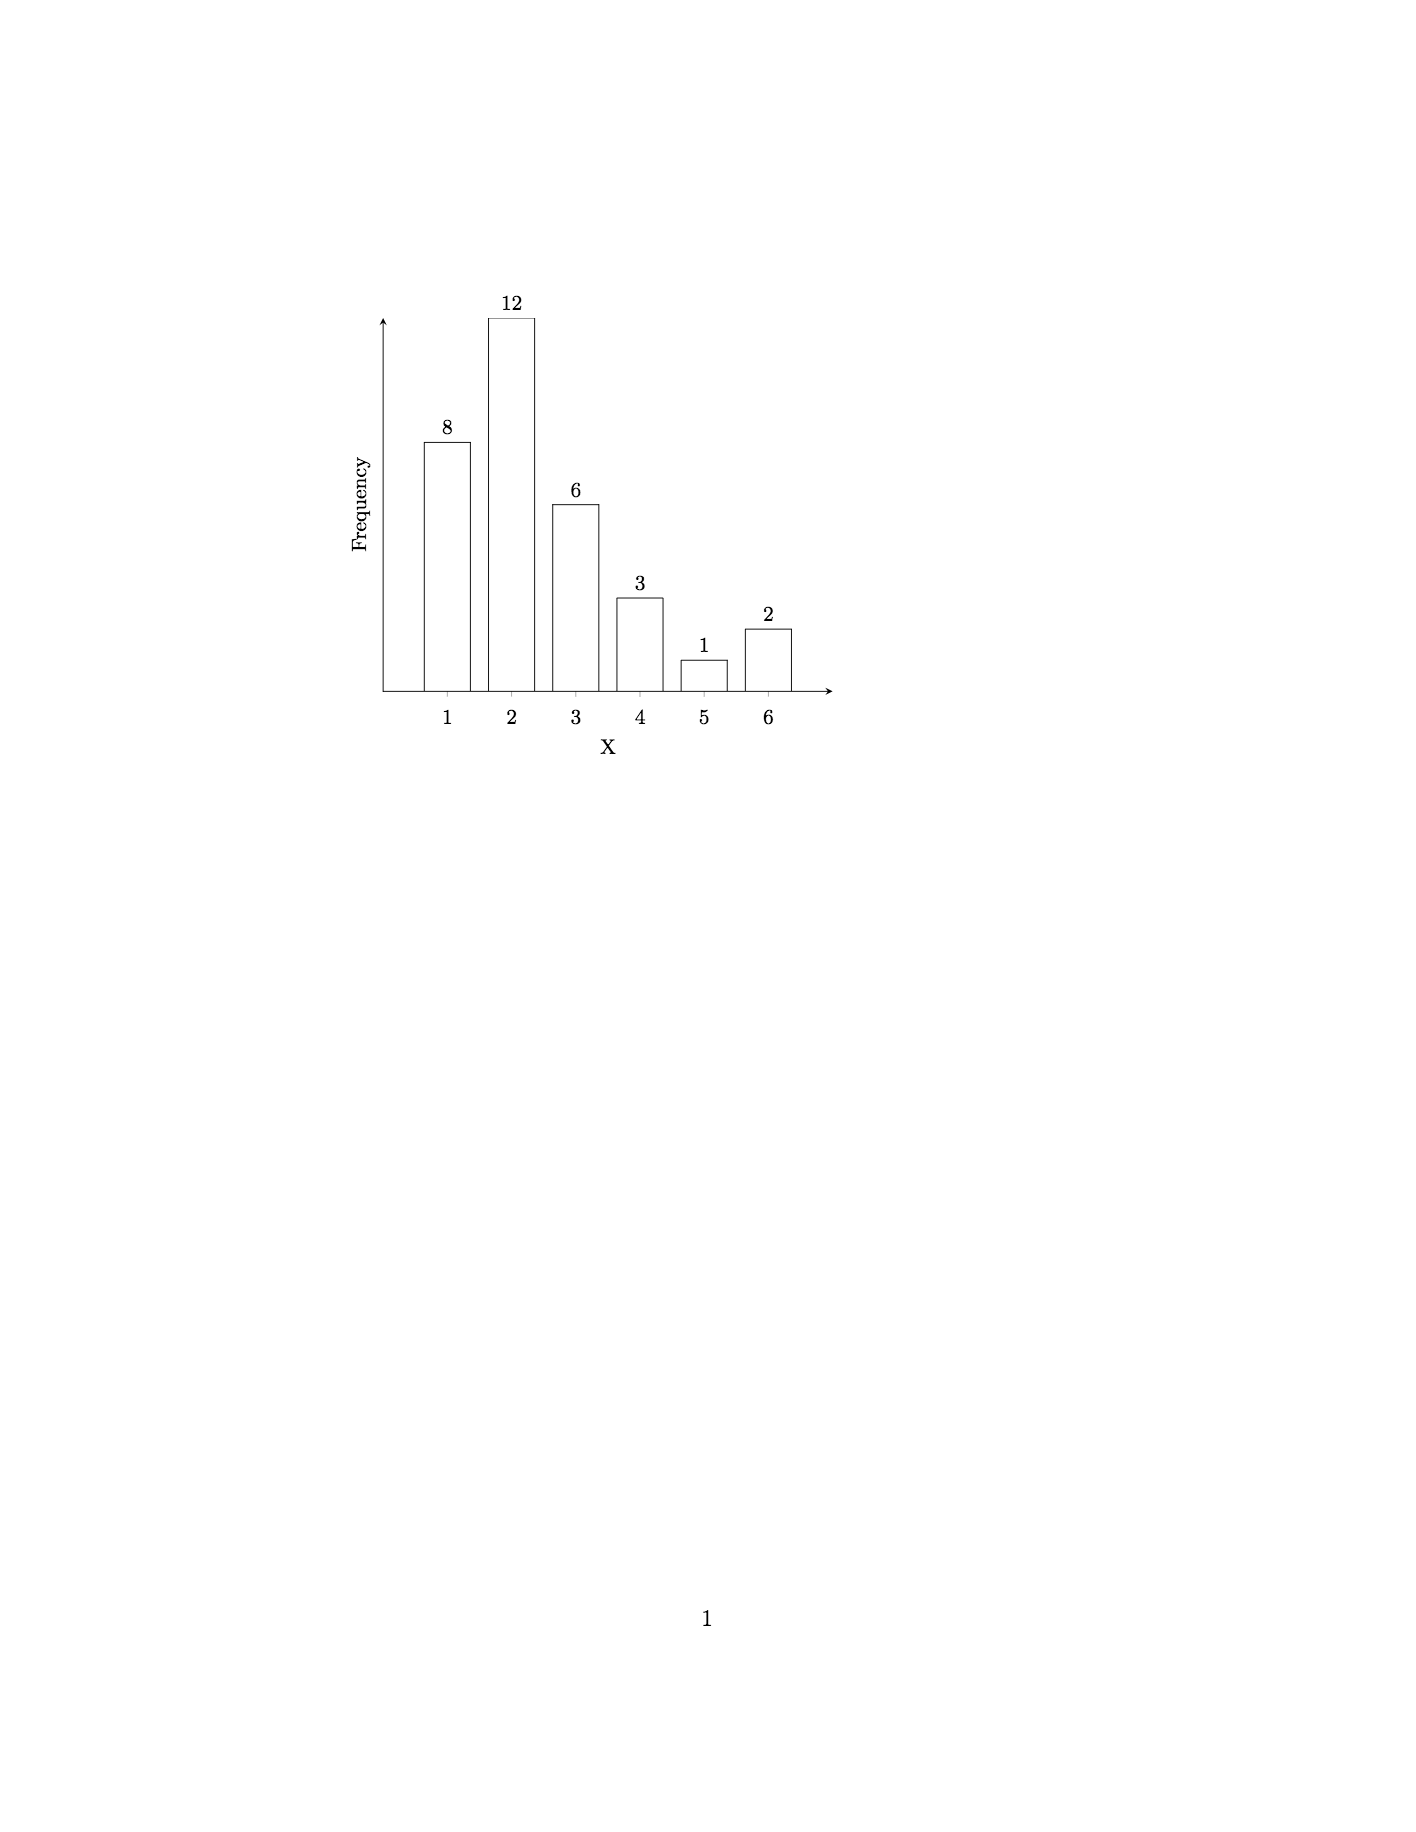
\includegraphics[width=1\linewidth]{images/frequencyhistogram.png}

		
		
%
\par
Experiment with creating your own histogram by inputting your data into the interactive cell below.
\begin{lstlisting}[style=sageinput]
#  This function is used to convert an input string into separate entries
def g(s): return str(s).replace(',',' ').replace('(',' ').replace(')',' ').split()

@interact
def _(freq = input_box("1,1,1,1,2,2,2,3,3,3,3,1,5",label="Enter data separated by commas")):
    freq = g(freq)
    freq = [int(k) for k in freq]
    m = min(freq)
    M = max(freq)
    bn = M-m+1
    histogram( freq, range=[m-1/2,M+1/2], bins = bn, align="mid", linewidth=2, edgecolor="blue", color="yellow").show()
\end{lstlisting}


		%
\par
Relative Frequency Histograms - In this case, area describes your data.  Notice in the interactive cell above that each bar is of width one. Therefore, frequency = area. In some instances where data may be grouped the total width of the interval may be different and so the height will need to be adjusted so that the total area of each bar corresponds to the relative frequency of that category.%
\par
Cummulative Histograms.  In these a running total is presented using all values from the given point and below.
\begin{lstlisting}[style=sageinput]
#  This function is used to convert an input string into separate entries
def g(s): return str(s).replace(',',' ').replace('(',' ').replace(')',' ').split()

@interact
def _(freq = input_box("1,1,1,1,2,2,2,3,3,3,3,1,5",label="Enter data separated by commas")):
    freq = g(freq)
    freq = [int(k) for k in freq]
    top = len(freq)
    m = min(freq)
    M = max(freq)
    bn = M-m+1
    histogram( freq, range=[m-1/2,M+1/2], cumulative = "true", bins = bn, align="mid", linewidth=2, edgecolor="blue", color="yellow").show(ymax=top)
\end{lstlisting}
		
		%
\par
Stem-and-Leaf Plot - Histogram with data. Using the state population data above, consider organizing the data but using a "two-pass sort" where you first roughly break data up into groups based upon ranges which relate to their first digit(s). In this case, let's break up into groups according to populations corresponding to 0-4 million, 5-9 million, 10-14 million, 15-19, million, 20-24 million, 25-29 million, 30-35 million, and 35-39 million. We can represent these classes by using the stems 0L, 0H, 1L, 1H, 2L, 2H, 3L, and 3H where the L and H represent the one's digits L in {0, 1, 2, 3, 4} and H in {5, 6, 7, 8, 9}.  Once we group the data into these smaller groups then we can write the remaining portion of the number horizontally as leaves (in this case with one decimal place for all values.) This gives a step-and-leaf plot. If we additionally sort the data in the leaves then this gives you an ordered stem-and-leaf plot. For the state population data, the ordered stem-and-leaf plot is given by
		
	
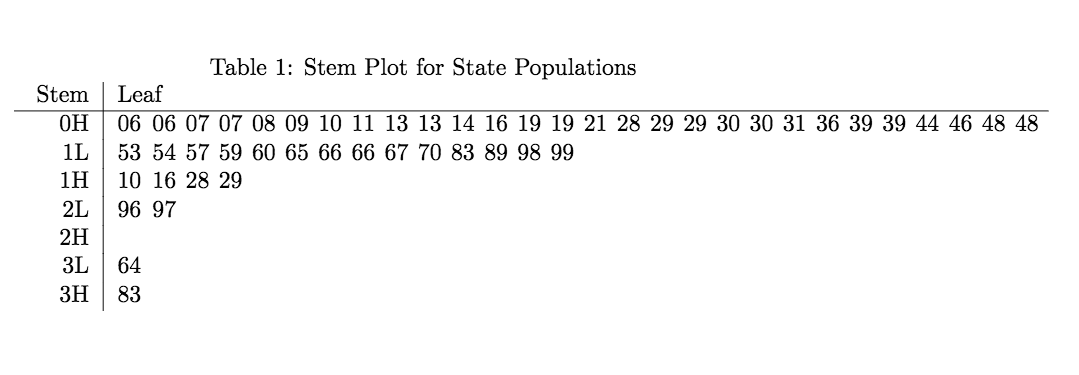
\includegraphics[width=1\linewidth]{images/stemandleaf.png}


Notice how it is easy to now see that most state populations are relatively small and that there are relatively few states with larger population. Also, notice that you can use this plot to relatively easily identify minimum, maximum, and other order statistics.		
		
		%
\par
Box and Whisker Diagram - visual order statistics. This graphical display identifies the "5-number-summary" associated with the minimum, quartiles, and the maximum. That is, \(y_1, Q_1, Q_2, Q_3, y_n\).  These values separate the data roughly into quarters. To distinguish these quarters connect \(y_1\) and \(Q_1\) with a straight line (a whisker) and do the same with \(Q_3\) and \(y_n\). Use a box to connect \(Q_1\) with \(Q_2\) and the same to connect \(Q_2\) with \(Q_3\). Then the boxed areas also identify the IQR.    
\begin{lstlisting}[style=sageinput]
from pylab import boxplot,savefig,close
@interact
def _(data = input_box([1,2,3,4,6,7,8,9,11,15,21],label="Enter Your Data:")):
    B = boxplot(data, notch=True, sym='x', vert=False)
    savefig("boxplot.png")
    close()
\end{lstlisting}

		%
\typeout{************************************************}
\typeout{Section 1.9 Exercises}
\typeout{************************************************}
\section[{Exercises}]{Exercises}\label{section-9}
Complete the online homework "Computational Measures".%
\begin{exercise}\label{exercise-3}
Create a data set with about 10 elements. For your data set, compute each of the measures from this chapter and present your data using a frequency histogram.%
\end{exercise}
\begin{exercise}\label{exercise-4}
Find a "real-world" data set (similar perhaps to the Census data presented above.) Compute each of the measures from this chapter. Interpret and present your conclusions in an electronic report which can include an excel spreadsheet.%
\end{exercise}
\typeout{************************************************}
\typeout{Chapter 2 Regression}
\typeout{************************************************}
\chapter[{Regression}]{Regression}\label{CurveEstimation}
\typeout{************************************************}
\typeout{Section 2.1 Introduction}
\typeout{************************************************}
\section[{Introduction}]{Introduction}\label{section-10}

Given two distinct points, there is one line which passes exactly through both.  Indeed, if the points are \((x_0,y_0), (x_0,y_0)\) then presuming the x-values are different gives the equation
\begin{equation*} y = \frac{y_1 - y_0}{x_1 - x_0}(x - x_0) + y_0\end{equation*}
is the linear function which passes through both points.  If the x's are equal then 
\begin{equation*} x = x_0\end{equation*}
is your linear equation. 
However, once you collect three or more points it is likely that there is no line which exactly "interpolates" all of the points.
%
\par

In this chapter, you will investigate how to create polynomial functions which in some manner approximate a collection of data point in some "best" manner.
%
\typeout{************************************************}
\typeout{Section 2.2 Linear Regression}
\typeout{************************************************}
\section[{Linear Regression}]{Linear Regression}\label{section-11}

In this section, we will presume only one independent variable x and one dependent variable y.
%
\par

Consider a collection of data points 
\begin{equation*}(x_1,y_1), (x_2,y_2), ... , (x_n,y_n)\end{equation*}
and a general linear function 
\begin{equation*}f(x) = mx + b.\end{equation*}
It is possible that each of the given data points are exactly "interpolated" by the linear function so that
\begin{equation*}f(x_k) = y_k\end{equation*}
for k = 1, 2, ... , n.  However, in general this is unlikely since even three points are not likely to be colinear. However, you may notice that the data points exhibit a linear tendency or that the underlying physics might suggest a linear model. If so, you may find it easier to predict values of y for given values of x using a linear approximation. Here you will investigate a method for doing so called "linear regression", "least-squares", or "best-fit line".
%
\par

To determine a best-fit line, you need to determine what is meant by the word "best". Here, we will derive the standard approach which interprets this to mean that the total vertical error between the line and the provided data points is minimized in some fashion.  Indeed, this vertical error would be of the form
\begin{equation*}e_k = f(x_k) - y_k\end{equation*}
and would be zero if f(x) exactly interpolated at the given data point.  Note, some of these errors will be positive and some will be negative. To avoid any possible cancellation of errors, you can look at taking absolute values (which is tough to deal with algebraically) or by squaring the errors. This second option will be the approach taken here. This is similar to the approach taken earlier when developing formulas for the variance.
%
\par
The best-fit line therefore will be the line \(f(x) = mx+b\) so that the "total squared error" is minimized. This total squared error is given by
\begin{equation*}TSE(m,b) = \sum_{k=1}^n e_k^2 = \sum_{k=1}^n (f(x_k) - y_k)^2 = \sum_{k=0}^n (m x_k + b - y_k)^2.\end{equation*}
To minimize this function of the two variables m and b, take partial derivatives and set them equal to zero to get the critical values:
\begin{equation*}TSE_m = \sum_{k=1}^n 2(m x_k + b - y_k) \cdot x_k\end{equation*}
and
\begin{equation*}TSE_b = \sum_{k=1}^n 2(m x_k + b - y_k) \cdot 1 .\end{equation*}
Setting equal to zero and solving gives what is known as the "normal equations":
\begin{equation*}m \sum_{k=1}^n x_k^2 + b \sum_{k=1}^n x_k = \sum_{k=1}^n x_k y_k\end{equation*}
and
\begin{equation*}m \sum_{k=1}^n x_k + b \sum_{k=1}^n 1 = \sum_{k=1}^n y_k.\end{equation*}
Solving these for m and b gives the best fit line.
%
\typeout{************************************************}
\typeout{Section 2.3 Higher Degree Regression}
\typeout{************************************************}
\section[{Higher Degree Regression}]{Higher Degree Regression}\label{section-12}

Continuing in a similar fashion to the previous section, consider now an approximation using a quadratic function \(f(x) = ax^2 + bx + c\).  In this case, the total squared error would be of the form
\begin{equation*}TSE(a,b,c) = \sum_{k=0}^n (a x_k^2 + b x_k + c - y_k)^2.\end{equation*}
Taking all three partials gives
\begin{equation*}TSE_a = \sum_{k=1}^n 2(a x_k^2 + b x_k + c - y_k) \cdot x_k^2\end{equation*}
\begin{equation*}TSE_b = \sum_{k=1}^n 2(a x_k^2 + b x_k + c - y_k) \cdot x_k\end{equation*}
\begin{equation*}TSE_c = \sum_{k=1}^n 2(a x_k^2 + b x_k + c - y_k) \cdot 1 .\end{equation*}
Once again, setting equal to zero and solving gives the normal equations for the best-fit quadratic
\begin{equation*}a \sum_{k=1}^n x_k^4 + b \sum_{k=1}^n x_k^3 + c \sum_{k=1}^n x_k^2 = \sum_{k=1}^n x_k^2 y_k\end{equation*}
\begin{equation*}a \sum_{k=1}^n x_k^3 + b \sum_{k=1}^n x_k^2 + c \sum_{k=1}^n x_k = \sum_{k=1}^n x_k y_k\end{equation*}
\begin{equation*}a \sum_{k=1}^n x_k^2 + b \sum_{k=1}^n x_k + c \sum_{k=1}^n 1 = \sum_{k=1}^n y_k.\end{equation*}


%
\typeout{************************************************}
\typeout{Chapter 3 Counting and Combinatorics}
\typeout{************************************************}
\chapter[{Counting and Combinatorics}]{Counting and Combinatorics}\label{Combinatorics}
\typeout{************************************************}
\typeout{Section 3.1 Introduction}
\typeout{************************************************}
\section[{Introduction}]{Introduction}\label{section-13}
Discussion on the usefulness of having ways to count the number
of elements in a set without having to explicitly listing all elements.%
\par
Consider counting the number of ways one can arrange Peter, Paul, and Mary with the order important.  Listing the possibilities:
\leavevmode%
\begin{itemize}[label=\textbullet]
\item{}Peter, Paul, Mary%
\item{}Peter, Mary, Paul%
\item{}Paul, Peter, Mary%
\item{}Paul, Mary, Peter%
\item{}Mary, Peter, Paul%
\item{}Mary, Paul, Peter%
\end{itemize}

So, it is easy to see that these are all of the possible outcomes and that the total number of such outcomes is 6. What happens however if we add Simone to the list?
\leavevmode%
\begin{itemize}[label=\textbullet]
\item{}Simone, Peter, Paul, Mary%
\item{}Simone, Peter, Mary, Paul%
\item{}Simone, Paul, Peter, Mary%
\item{}Simone, Paul, Mary, Peter%
\item{}Simone, Mary, Peter, Paul%
\item{}Simone, Mary, Paul, Peter%
\item{}Peter, Simone, Paul, Mary%
\item{}Peter, Simone, Mary, Paul%
\item{}Paul, Simone, Peter, Mary%
\item{}Paul, Simone, Mary, Peter%
\item{}Mary, Simone, Peter, Paul%
\item{}Mary, Simone, Paul, Peter%
\item{}Peter, Paul, Simone, Mary%
\item{}Peter, Mary, Simone, Paul%
\item{}Paul, Peter, Simone, Mary%
\item{}Paul, Mary, Simone, Peter%
\item{}Mary, Peter, Simone, Paul%
\item{}Mary, Paul, Simone, Peter%
\item{}Peter, Paul, Mary, Simone%
\item{}Peter, Mary, Paul, Simone%
\item{}Paul, Peter, Mary, Simone%
\item{}Paul, Mary, Peter, Simone%
\item{}Mary, Peter, Paul, Simone%
\item{}Mary, Paul, Peter, Simone%
\end{itemize}

Notice how the list quickly grows when just adding one more choice. This illustrates how keeping track of the number of items in a set can quickly get impossible to keep up with and to count unless we can approach this problem using a more mathematical approach.
%
\begin{definition}[{Cardinality}]\label{definition-14}
Given a set of elements A, the number of elements in the 
		set is known as the sets cardinality and is denoted |A|. If the set has 
		an infinite number of elements then we set |A| = \(\infty\).
		\end{definition}
\par
In order to "count without counting" we establish the following 
	foundational principle.%
\begin{theorem}[{Multiplication Principle}]\label{theorem-3}
Given two successive events A and B, the number of ways 
		to perform A and then B is |A||B|.
		\end{theorem}
\begin{proof}\hypertarget{proof-3}{}
If either of the events has infinite cardinality, then it is 
			clear
			that the number of ways to perform A and then B will also be 
			infinite. So, assume that both |A| and |B| are finite.
			In order to count the successive events, enumerate the elements in
			each set
			\begin{gather*}
A = \left \{ a_1, a_2, a_3, ... , a_{|A|} \right \}\\
B = \left \{  b_1, b_2, b_3, ... , b_{|B|} \right \}
\end{gather*}
			and consider the function f(k,j) = (k-1)|B| + j. This function is 
			one-to-one and onto from the set 
			\begin{gather*}
\left \{ (k,j): 1 \le k \le |A|, 1 \le j \le |B| \right \} 
\end{gather*} 
			onto 
			\begin{gather*}
\left \{ s : 1 \le s \le |A| |B| \right \}.
\end{gather*} 
			Since this
			second set has |A| |B| elements then the conclusion follows. 
			coordinates.%
\end{proof}
\begin{definition}[{Factorial}]\label{definition-15}
For any natural number n, 
		\begin{gather*}
n! = n(n-1)(n-2) ... 3 \cdot 2 \cdot 1
\end{gather*}
		and by convention set 0! = 1.
		%
\end{definition}
\begin{example}[iPad security code]\label{example-6}
Consider your ipad's security. To unlock the screen you need to enter your four digit pass code. How easy is it to guess this pass code?%
\par
Using the standard 10 digit keypad, we first have two questions to consider?
		\leavevmode%
\begin{enumerate}
\item\hypertarget{li-63}{}Does the order in which the digits are entered matter?%
\item\hypertarget{li-64}{}Can you reuse a digit more than once?%
\end{enumerate}

		For the ipad, the order does matter and you cannot reuse digits. In this case, the number of possible codes can be determined by considering each digit as a separate event with four such events in succession providing the right code. By successively applying the multiplication principle, you find that the number of possible codes is the number of remaining available digits at each step.  Namely, \(10 \times 9 \times 8 \times 7 = 5040.\)
		%
\par

		Note that if you were allowed to reuse the digits then the number of possible outcomes would be more since all 10 digits would be available for each event.  Namely, \(10 \times 10 \times 10 \times 10 = 10000.\)
		%
\end{example}
\begin{example}[iPad security code with greasy fingers]\label{example-7}
Reconsider your ipad's security. In this case, you like to eat
		chocolate bars and have greasy fingers. When you type in your passcode
		your fingers leave a residue over the four numbers pressed. If someone
		now tries to guess your passcode, how many possible attempts are necessary?%
\par
Since there are only four numbers to pick from with order important, the number of possible passcodes remaining is \(4 \times 3 \times 2 \times 1 = 24\)%
\end{example}
\begin{example}[National Treasure]\label{example-8}
In the 2004 movie National Treasure, Ben and Riley are attempting 
		to guess Abagail's password to enter the room with the Declaration. 
		They are able
		to determine the passphrase to get into the vault room by doing a scan
		that detects the buttons pushed (not due to chocolate but just due to 
		the natural oils on fingers). They notice that the buttons pushed 
		include the characters AEFGLORVY.%
\par
Assuming these characters are used only once each, how many possible
		passphrases are possible?%
\par

		In this case, the order of the characters matters but all of the 
		characters are distinct. Since we have 9 characters provided, the we can
		consider each character as an event with the first event as a choice
		from the 9, the second event as a choice from the remaining 8, etc. This
		gives \(9 \times 8 \ times ... \times 1 = 362880\) possible 
		passphrases.
		%
\par
Assuming that some of the characters could be used more than once, 
		how many passphrases need to be considered if the total length
		of passphrase can be at most 12 characters?%
\par
Notice, in this case you don't know which characters might be reused and so the number of possible outcomes will be much larger. What is the answer?%
\par
You can break this problem down into distinct cases:
		\leavevmode%
\begin{itemize}[label=\textbullet]
\item{}Using 9 characters: The answer was computed above.%
\item{}Using 10 characters: In this case, 1 character can be used twice. To determine the number of possibilities, let's first pick which character can be doubled. There are 9 options for picking that character.  Next, if we consider the two instances of that letter as distinct values then we can just count the number of ways to arrange unique 10 characters which is 10! However, swapping the two characters (which are actually identical) would not give a new passphrase. Since these are counted twice, let's divide these out to give 10!/2.%
\item{}Using 11 characters:In this situation we have two unique options:
				%
\begin{itemize}[label=$\circ$]
\item{}One character is used three times and the others just once.%
\par
Continuing as in the previous case, 11!/3!.%
Two characters are used twice and the others just once.\end{itemize}

				%
\item{}Using 12 characters%
%
\begin{enumerate}
\item\hypertarget{li-71}{}One letter from the nine is used four times and all the others are used once.%
\item\hypertarget{li-72}{}One letter is used three times, another letter is used two times, and the others are used once.%
\item\hypertarget{li-73}{}Three letters are used twice and the others are used once.%
\end{enumerate}
\end{itemize}

			%
\par
With this large collection of possible outcomes, how are the movie
		characters able to determine the correct "VALLEYFORGE" passphrase?%
\end{example}
\typeout{************************************************}
\typeout{Section 3.2 Permutations}
\typeout{************************************************}
\section[{Permutations}]{Permutations}\label{section-14}
When counting various outcomes the order of things sometimes matters. When the order of a set of elements changes we call the second a permutation (or an arrangement) of the first.%
\begin{theorem}[{Permutations of everything}]\label{theorem-4}
The number of ways to arrange n distinct items is n!\end{theorem}
\begin{proof}\hypertarget{proof-4}{}
Notice that if n=1, then there is only 1 item to arrange and 
			that there is only one possible arrangment.%
\par

			By induction, assume that any set with n elements has n! arrangments 
			and assume that 
			\begin{gather*}
|A| = \left \{ a_1, a_2, ... , a_n, a_{n+1} \right \}.
\end{gather*}
			Notice that there are n+1 ways to choose 1 element from A and that in doing so leaves a set with n elements. Combining the induction hypothesis with the multiplication principle this gives (n+1)n! = (n+1)! possible outcomes.
			%
\end{proof}
\begin{theorem}[{Permutations of a subset without replacement}]\label{theorem-5}
 
			The number of ways to arrange r items from a set of n distinct items 
			is 
			\begin{equation*} P_r^n = \frac{n!}{(n-r)!} \end{equation*}
			%
\end{theorem}
\begin{proof}\hypertarget{proof-5}{}

			If \(r \gt n\) or \(r \lt 0 \) then this is not possible and so the result would be no permuatations. Otherwise, apply the multiplication principle r times noting that there are 
			n choices for the first selection, n-1 choices for the second
			selection, and with n-r+1 choices for the rth selection. This gives
			\begin{align*}
P_r^n & = n(n-1) ... (n-r+1)\\
& = n(n-1) ... (n-r+1)\frac{(n-r)!}{(n-r)!}\\
& = \frac{n(n-1) ... (n-r+1)(n-r)!}{(n-r)!}\\
& = \frac{n!}{(n-r)!}
\end{align*}
			%
\end{proof}
\begin{theorem}[{Permutations of a subset with replacement}]\label{theorem-6}
The number of ways to obtain an arrangement of r choices from a group of size n is 
		\begin{equation*}n^r\end{equation*}\end{theorem}
\begin{proof}\hypertarget{proof-6}{}

			Use the multiplication principle r times and see that for each choice all n objects in the universe remain available.  That is, 
			\begin{equation*}n \cdot n \cdot n ... n = n^r\end{equation*}
			%
\end{proof}
\begin{theorem}[{Permutations when not all items are distinguishable (Multinomial Coefficients)}]\label{theorem-7}

If n items belong to s categories, \(n_1\) in first, \(n_2\) in second, ... , \(n_s\) in the last, the number of ways to pick all is
		\begin{equation*}\frac{n!}{n_1! \cdot n_2! ... n_2!}\end{equation*}\end{theorem}
\typeout{************************************************}
\typeout{Section 3.3 Combinations}
\typeout{************************************************}
\section[{Combinations}]{Combinations}\label{section-15}
When counting various outcomes sometimes the order of things does not matter.
In this case we count each different set of outcomes a combination. %
\begin{theorem}[{Combinations of a subset without replacement}]\label{theorem-8}

			The number of ways to arrange r items from a set of n distinct items 
			is 
			\begin{equation*} C_r^n = \frac{n!}{r!(n-r)!} \end{equation*}
			%
\end{theorem}
\begin{proof}\hypertarget{proof-7}{}

			Consider creating a permutation of r objects from a set of size n
			by first picking an unordered subset of size r and then counting 
			the number of ways to order that subset. Using our notation and the
			multiplication principle,
			\begin{gather*}
P_r^n = C_r^n \cdot r!
\end{gather*}
			Solving give the result.
			%
\end{proof}
\begin{theorem}[{Combinations of a subset with replacement}]\label{theorem-9}

			The number of ways to arrange r items from a set of n distinct items 
			is 
			\begin{equation*} C_r^{n+r-1} = \frac{(r+n-1)!}{r!(n-1)!} \end{equation*}
			%
\end{theorem}
\begin{proof}\hypertarget{proof-8}{}

			Label each item in your group in some defined order. Since order doesn't matter, as you repeatedly sample r times with replacement you can always write down your outcomes sorted from low to high placement. Finally, separate like values by some symbol, say "|", and consider each of the n distinct objects as indistinct *'s. There will be n-1 of these separators since there will be n to choose from. For example, if choosing r=6 times from the set {a, b, c, d}, then the outcome b, b, a, d, a, b could be collected as a, a, b, b, b, d and written in our code as **|***||* .  Notice that shuffling around the identical *'s would not change the code (and similarly for the identical |'s) but swapping a * with a | would be a different outcome. Therefore, we can consider this to be a multinomial coefficient and the number of ways to rearrange this code is
			\begin{equation*}\frac{(r + n-1)}{r!(n-1)!}.\end{equation*}
			%
\end{proof}
\begin{example}[Ipad Security]\label{example-9}
Revisiting your ipad's security, what happens if the order in which the digits are entered does not matter? If so, then you would be picking a combination of 4 digits without replacement from a group of 10 digits. Namely, 
		\begin{align*}
\frac{10!}{4!6!} & = \frac{10 \times 9 \times 8 \times 7 \times 6!}{4 \times 3 \times 2 \times 1 \times 6!}\\
& = \frac{10 \times 9 \times 8 \times 7}{4 \times 3 \times 2 \times 1}\\
& = \frac{5040}{24}\\
& = 210.
\end{align*}
		Notice that the total number of options is much smaller when order does not matter.
		%
\par

		Note that if you were allowed to reuse the digits then the number of possible outcomes would be
		\begin{align*}
\frac{13!}{3!10!} & = \frac{13 \times 12 \times 11}{3 \times 2 \times 1} \\
 & = 286
\end{align*}
		which once again is more since numbers are allowed to repeat.
		%
\end{example}
\begin{definition}[{Binomial Coefficients}]\label{definition-16}

		The value \(C_r^n\) is known as the binomial coefficient. It is
		denoted by \({n \choose r}\) and is read "n choose k".
		%
\end{definition}
\par
Binomial coefficients have a number of interesting properties.  Many of these are very useful as well in probability calculations.  Several of these properties are collected below. In particular, these relationships verify that the binomial coefficients are the values found in Pascal's Triangle.%
\begin{theorem}[{ Binomial Coefficient Formulas}]\label{theorem-10}
 For \( n \in \mathbb{N}\),
	\leavevmode%
\begin{enumerate}
\item\hypertarget{li-74}{}\(\binom{n}{0} = 1\)%
\item\hypertarget{li-75}{}\(\binom{n}{n} = 1\)%
\item\hypertarget{li-76}{}\(\binom{n}{1} = n\)%
\item\hypertarget{li-77}{}\(\binom{n}{n-1} = n\)%
\item\hypertarget{li-78}{}\(\binom{n}{r} = \binom{n}{n-r}\)%
\item\hypertarget{li-79}{}\(\binom{n+1}{r+1} = \binom{n}{r} + \binom{n}{r+1}\)%
\end{enumerate}

	%
\end{theorem}
\begin{proof}\hypertarget{proof-9}{}

	\leavevmode%
\begin{enumerate}
\item\hypertarget{li-80}{}\(\binom{n}{0} = \frac{n}{0!(n-0)!} = 1\)%
\item\hypertarget{li-81}{}\(\binom{n}{n} = \frac{n}{n!(n-n)!} = 1\)%
\item\hypertarget{li-82}{}\(\binom{n}{1} = \frac{n}{1!(n-1)!} = n\)%
\item\hypertarget{li-83}{}\(\binom{n}{n-1} = \frac{n}{(n-1)!(n-(n-1))!} = n\)%
\item\hypertarget{li-84}{}\(\binom{n}{r} = \frac{n}{r!(n-r)!} = \frac{n!}{(n-r)!(n-(n-r))!} = \binom{n}{n-r}\)%
\item\hypertarget{li-85}{}
		\begin{align*}
\binom{n}{r} + \binom{n}{r+1} & = \frac{n!}{r!(n-r)!} + \frac{n!}{(r+1)!(n-(r+1))!}\\
 & = (r+1) \frac{n!}{(r+1)!(n-r)!} + (n-r) \frac{n!}{(r+1)!(n-r))!}\\
 & = \frac{(r+1) n! + (n-r)n!}{(r+1)!(n-r)!}\\
 & = \frac{(n+1) n!}{(r+1)!((n+1)-(r+1))!}\\
 & = \binom{n+1}{r+1}
\end{align*}
		%
\end{enumerate}

	%
\end{proof}
\typeout{************************************************}
\typeout{Section 3.4 Exercises}
\typeout{************************************************}
\section[{Exercises}]{Exercises}\label{section-16}
Complete the online homework "Counting".%
\par

A standard deck of playing cards consists of 52 cards broken up into four "suits" known as Hearts, Spades, Diamonds, and Clubs. Each suit is broken up additionally into unique cards with "face values" from {2, 3, 4, 5, 6, 7, 8, 9, 10, Jack, Queen, King, Ace} and generally in that order from low to high.%
\par

1.  Pick two cards without replacement one after the other from this deck and determine the following number of possible outcomes:
\leavevmode%
\begin{itemize}[label=\textbullet]
\item{}The number of ways to get an Ace for both cards.%
\item{}The number of ways to get an Ace for only one of the two cards.%
\item{}The number of ways to get an Ace on the first draw and a Spade on the second draw.%
\end{itemize}

2.  Pick five cards without replacement one after the other from a newly shuffled full deck and determine the following number of possible outcomes:
\leavevmode%
\begin{itemize}[label=\textbullet]
\item{}All cards have different faces%
\item{}"A pair". That is, two cards have the same face but the others are from three other faces.%
\item{}"Three of a kind".  That is, three cards have the same face but the others are from two other faces.%
\item{}"Two Pair". That is, two cards come from one face, two other cards come from a common face that is not the same as the first two cards, and the last card comes from some other face.%
\item{}"Full House". That is, three cards have the same face and the other two come from a common face that is not the same as the first three cards.%
\item{}"Four of a Kind". That is, four cards have the same face and the other card comes from some other face.%
\item{}"Flush". That is, the five cards for a sequence in order of adjacent faces in the original list and from the same suit.%
\item{}"Royal Flush". That is, a flush but only with the cards {Ace, King, Queen, Jack, 10}.%
\end{itemize}

%
\par
Completely determine the number of possible passphrases for the National Treasure example started above. Present your answer in a report form.%
\typeout{************************************************}
\typeout{Chapter 4 Probability Theory}
\typeout{************************************************}
\chapter[{Probability Theory}]{Probability Theory}\label{ProbabilityGeneralities}
\typeout{************************************************}
\typeout{Section 4.1 Introduction}
\typeout{************************************************}
\section[{Introduction}]{Introduction}\label{section-17}
This chapter uses relative frequency to motivate the definition of probability and then delves into the resulting consequences.%
\par
Mathematics generally focuses on providing precise answers with absolute certainty. For example, solving an equation generates specific (and non-varying) solutions. Statistics on the other hand deals with providing precise answers to questions when there is uncertainty. It might seem impossible to provide such precise answers but the focus of this text is to show how that can be done so long as the questions are properly posed and the answers properly interpreted.%
\par
People often make claims about being the biggest, best, most often recommended, etc. One sometimes even believes these claims. In this class, we will attempt to determine if such claims are reasonable by first introducing probability from a semi rigorous mathematical viewpoint using concepts developed in Calculus. We will use this framework to carefully discuss making such statistical inferences as above and in general to obtain accurate knowledge even when the known data is not complete. %
\typeout{************************************************}
\typeout{Section 4.2 Relative Frequency}
\typeout{************************************************}
\section[{Relative Frequency}]{Relative Frequency}\label{RelativeFrequency}
When attempting to precisely measure uncertainty a few experiments are in order. When doing statistical experiments, a few terms and corresponding notation might be useful:%
\leavevmode%
\begin{itemize}[label=\textbullet]
\item{}S = Universal Set or Sample Space Experiment or Outcome Space. 
		This is the collection of all possible outcomes.%
\item{}Random Experiment. A random experiment is a repeatable activity which has more than one
		possible outcome all of which can be specified in advance but can not be known in advance with certainty.%
\item{}Trial. Performing a Random Experiment one time and measuring the result.%
\item{}A = Event. A collection of outcomes.  Generally denoted by an upper case letter such as A, B, C, etc.%
\item{}Success/Failure. When recording the result of a trial, a success for event A occurs when the outcome
		lies in A. If not, then the trial was a failure. There is no qualitative meaning to this term.%
\item{}Mutually Exclusive Events. Two events which share no common outcomes. Also known as disjoint events.%
\item{}|A| = Frequency. In a sequence of n events, the frequency is the number of trials which resulted in 
		a success for event A.%
\item{}|A| / n = Relative Frequency. A proportion of successes to total number of trials.%
\item{}Histogram. A bar chart representation of data where area corresponds to the value being described.%
\end{itemize}
\par
To investigate these terms and to motivate our discussion of probability, consider flipping coins using the interactive cell below. Notice in this case, the sample space S = {Heads, Tails} and the random experiment consists of flipping a fair coin one time. Each trial results in either a Head or a Tail. Since we are measuring both Heads and Tails then we will not worry about which is a success or failure. Further, on each flip the outcomes of Heads or Tails are mutually exclusive events. We count the frequencies and compute the relative frequencies for a varying number of trials selected by you as you move the slider bar. Results are displayed using a histogram.%
\par

	Question 1: What do you notice as the number of flips increases?
	%
\par

	Question 2: Why do you rarely (if even) get exactly the same number of Heads and Tails? Would you not "expect"
	that to happen?
	%
\begin{lstlisting}[style=sageinput]
coin = ["Heads", "Tails"]
@interact
def _(num_rolls = slider([5..5000],label="Number of Flips")):
	rolls = [choice(coin) for roll in range(num_rolls)]
	show(rolls)   
	freq = [0,0]
	for outcome in rolls:
		if (outcome=='Tails'):
			freq[0] = freq[0]+1
		else:
			freq[1] = freq[1]+1
	print("\nThe frequency of tails = "+ str(freq[0]))+" and heads = "+ str(freq[1])+"."
	rel = [freq[0]/num_rolls,freq[1]/num_rolls]
	print("\nThe relative frequencies for Tails and Heads:"+str(rel))
	show(bar_chart(freq,axes=False,ymin=0))     #  A histogram of the results
\end{lstlisting}
\par
Notice that as the number of flips increases, the relative frequency of Heads (and Tails)
	stabilized around 0.5. This makes sense intuitively since there are two options for each 
	individual flip and 1/2 of those options are Heads while the other 1/2 is Tails.%
\par

	Let's try again
	by doing a random experiment consisting of rolling a single die one time. Note that the sample space 
	in this case will be the outcomes S = {1, 2, 3, 4, 5, 6}.
	%
\begin{exercise}\label{exercise-5}

		Let's see if you understand the relationship between frequency and relative frequency.
		%
\par\medskip
\mbox{}\\ % hack to move box after heading
\begin{mdframed}
{}\par\vspace*{2ex}%
{\tiny\ttfamily\noindent\url{Library/MC/PreAlgebra/setPreAlgebraC06S04/BasicProbability03.pg}\\Seed: \hfill}\end{mdframed}
\medskip\noindent 
		So, these are simple calculations.
		%
\par
\end{exercise}
\par

	Question 1: What do you notice as the number of rolls increases?
	%
\par

	Question 2: What do you expect for the relative frequencies and why are they not all exactly the same?
	%
\begin{lstlisting}[style=sageinput]
@interact
def _(num_rolls = slider([20..5000],label='Number of rolls'),Number_of_Sides = [4,6,8,12,20]):
	die = list((1..Number_of_Sides))
	rolls = [choice(die) for roll in range(num_rolls)]
	show(rolls)   

	freq = [rolls.count(outcome) for outcome in set(die)]  # count the numbers for each outcome
	print 'The frequencies of each outcome is '+str(freq)

	print 'The relative frequencies of each outcome:'
	rel_freq = [freq[outcome-1]/num_rolls for outcome in set(die)]  # make frequencies relative
	print rel_freq
	fs = []
	for f in rel_freq:
		fs.append(f.n(digits=4))
	print fs
	show(bar_chart(freq,axes=False,ymin=0))
\end{lstlisting}
\par
Notice in this instance that there are a larger number of options (for example 6 on a regular
	die) but once again the relative frequencies of each  outcome was close to 1/n (i.e. 1/6 for the regular die)
	as the number of rolls increased.%
\par
In general, this suggests a rule: if there are n outcomes and each one has the same
	chance of occurring on a given trial then on average on a large number of trials the relative
	frequency of that outcome is 1/n.
	In general, if a number of outcomes are "equally likely" then this is a good model for measuring
	the proportion of outcomes that would be expected to have any given outcome. However, it is not
	always true that outcomes are equally likely. Consider rolling two die and measuring their sum:%
\begin{lstlisting}[style=sageinput]
@interact
def _(num_rolls = slider([20..5000],label='Number of rolls'),num_sides = slider(4,20,1,6,label='Number of sides')):
    die = list((1..num_sides))
    dice = list((2..num_sides*2))
    rolls = [(choice(die),choice(die)) for roll in range(num_rolls)]
    sums = [sum(rolls[roll]) for roll in range(num_rolls)]
    show(rolls)   

    freq = [sums.count(outcome) for outcome in set(dice)]  # count the numbers for each outcome
    print 'The frequencies of each outcome is '+str(freq)
    
    print 'The relative frequencies of each outcome:'
    rel_freq = [freq[outcome-2]/num_rolls for outcome in set(dice)]  # make frequencies relative
    print rel_freq        
    show(bar_chart(freq,axes=False,ymin=0))     #  A histogram of the results
    print "Relative Frequence of ",dice[0]," is about ",rel_freq[0].n(digits=4)
    print "Relative Frequence of ",dice[num_sides-1]," is about ",rel_freq[num_sides-1].n(digits=4)
\end{lstlisting}
\par
Notice, not only are the answers not the same but they are not even close. To understand why this 
	is different from the examples before, consider the possible outcomes from each pair of die. Since we
	are measuring the sum of the dice then (for a pair of standard 6-sided dice) the possible sums are from 
	2 to 12. However, there is only one way to get a 2--namely from a (1,1) pair--while there are 6 ways to get
	a 7--namely from the pairs (1,6), (2,5), (3,4), (4,3), (5,2), and (6,1). So it might make some sense
	that the likelihood of getting a 7 is 6 times larger than that of getting a 2. Check to see if that
	is the case with your experiment above.%
\typeout{************************************************}
\typeout{Section 4.3 Definition of Probability}
\typeout{************************************************}
\section[{Definition of Probability}]{Definition of Probability}\label{section-19}
\typeout{************************************************}
\typeout{Introduction  }
\typeout{************************************************}

		Relative frequency gives a way to measure the proportion of "successful" outcomes when doing an experimental approach. From the interactive applications above, it appears that the relative frequency does jump around as the experiment is repeated but that the amount of variation decreases as the number of experiments increases. This is known to be true in general and leads to what is known as the "Law of Large Numbers". We would like to formalize what these relative frequencies seem to be approaching and will call this theoretical limit the "probability" of the outcome. In doing so, we will do our best to model our definition so that it follow the behavior of relative frequency.
		%
Using the ideas from our examples above, consider how you might formally define a way
	to measure the expectation from similar experiments.  Before doing so, we need a little notation:%
\begin{definition}[{Pairwise Disjoint Sets}]\label{definition-17}

	\( \{ A_1, A_2, ... , A_n \}\) are pairwise disjoint provided \(A_k \cap A_j = \emptyset\) so long as \(k \ne j\).
	Disjoint sets as also often called mutually exclusive.
	%
\end{definition}
\par

	To model the behavior above, consider how we might create a definition for our expectation
	of a given outcome by following the ideas uncovered above. To do so, first consider a desired collection
	of outcomes A. If each outcome in A is equally likely then we might follow the concept behind relative 
	frequency and consider a measure of expectation be |A|/|S|. Indeed, on a standard 
	6-sided die, the expectation of the outcome A={2} from the collection S = {1,2,3,4,5,6} should be
	|A|/|S| = 1/6.%
\par
From the example where we take the sum of two die, the outcome A={4,5} from the
	collection S = {2,3,4,...,12} would be%
\begin{gather*}
|A| = | {(1,3),(2,2),(3,1),(1,4),(2,3),(3,2),(4,1)}| = 7\\
|S| = | {(1,1),...,(1,6),(2,1),...,(2,6),...,(6,1),...,(6,6)}| = 36
\end{gather*}\par
and so the expected relative frequency would be |A|/|S| = 7/36. Compare this theoretical value
	with the sum of the two outcomes from your experiment above.%
\par
We are ready to now formally give a name to the theoretical measure of expectation for
	outcomes from an experiment. Taking our cue from the ideas related to equally likely outcomes, we 
	make our definition have the following basic properties:%
\leavevmode%
\begin{enumerate}
\item\hypertarget{li-106}{}Relative frequency cannot be negative, since cardinality cannot be negative%
\item\hypertarget{li-107}{}Relative frequencies for disjoint events should sum to one%
\item\hypertarget{li-108}{}Relative frequencies for collections of disjoint outcomes should equal the sum of the
	individual relative frequencies%
\end{enumerate}
\par
Based upon these we give the following:%
\begin{definition}[{}]\label{DefnProb}
The probability P(A) of a given outcome A is a set function which satisfies:
		\leavevmode%
\begin{enumerate}
\item\hypertarget{li-109}{}(Nonnegativity) P(A) \(\ge 0\)%
\item\hypertarget{li-110}{}(Totality) P(S) = 1%
\item\hypertarget{li-111}{}(Subadditivity) If A \(\cap\) B = \(\emptyset\), then P(A \(\cup\) B) = P(A) + P(B).  
			In general, if {\(A_k\)} are pairwise disjoint then \(P( \cup_k A_k) = \sum_k P(A_k)\).%
\end{enumerate}
\end{definition}
\begin{exercise}\label{exercise-6}

		Using the definition above determine the following probabilities.  (This one not available
		in the PCC library for some reason.)
		%
\par\medskip
\mbox{}\\ % hack to move box after heading
\begin{mdframed}
{}\par\vspace*{2ex}%
{\tiny\ttfamily\noindent\url{Library/MC/PreAlgebra/setPreAlgebraC06S04/BasicProbability01.pg}\\Seed: \hfill}\end{mdframed}
\medskip\noindent 
		Notice when you are given complete information regarding the entire data set then determining
		probabilities for events can be relatively easy to compute.
		%
\par
\end{exercise}
\par
Based upon this definition we can immediately establish a number of results.%
\begin{theorem}[{Probability of Complements}]\label{ProbabilityComplemnts}
 For any event A, \(P(A) + P(A^c) = 1\)\end{theorem}
\begin{proof}\hypertarget{proof-10}{}
Let A be any event and note that \(A \cap A^c = \emptyset\).  But \(A \cup A^c = S\).
			So, by subadditivity \(1 = P(S) = P(A \cup A^c) = P(A) + P(A^c)\) as desired.%
\end{proof}
\begin{theorem}[{}]\label{ProbabilityEmptySet}
\(P(\emptyset) = 0\)\end{theorem}
\begin{proof}\hypertarget{proof-11}{}
Note that \(\emptyset^c = S\). So, by the theorem above, 
			\(1 = P(S) + P(\emptyset) \Rightarrow 1 = 1 + P(\emptyset)\).
			Cancelling the 1 on both sides gives \(P(\emptyset) = 0\). %
\end{proof}
\begin{theorem}[{}]\label{ProbabilityContainment}
For events A and B with \( A \subset B, P(A) \le P(B)\).
		\end{theorem}
\begin{proof}\hypertarget{proof-12}{}
Assume sets A and B satisfy \( A \subset B\). Then, notice that
			\(A \cap (B-A) = \emptyset\) and  \(B = A \cup (B-A)\). Therefore, by 
			subadditivity and nonnegativity%
\begin{gather*}
0 \le P(B-A)\\
P(A) \le P(A) + P(B-A) \\
P(A) \le P(B)
\end{gather*}\end{proof}
\begin{theorem}[{}]\label{ProbabilityLessThanOne}
For any event A, \(P(A) \le 1\)\end{theorem}
\begin{proof}\hypertarget{proof-13}{}
Notice \(A \subset S\). By the theorem above \( P(A) \le P(S) = 1\)%
\end{proof}
\begin{theorem}[{}]\label{ProbabilityTwoUnions}
For any sets A and B, \(P(A \cup B) = P(A) + P(B) - P(A \cap B)\)\end{theorem}
\begin{proof}\hypertarget{proof-14}{}
Notice that we can write \(A \cup B\) as the disjoint union%
\begin{gather*}
A \cup B = (A-B) \cup (A \cap B) \cup (B-A).
\end{gather*}\par
We can also write disjointly%
\begin{gather*}
A = (A-B) \cup (A \cap B)\\
B = (A \cap B) \cup (B-A)
\end{gather*}\par
Hence, %
\begin{align*}
P(A) & + P(B) - P(A \cap B) \\
& = [P(A-B) + P(A \cap B)] + [P(A \cap B) + P(B-A)] - P(A \cap B)\\
& = P(A-B) + P(A \cap B) + P(B-A)\\
& = P(A \cup B)
\end{align*}\end{proof}
\par
This result can be extended to more that two sets using a property known as inclusion-exclusion. The
	following two theorems illustrate this property and are presented without proof.
	%
\begin{corollary}[{}]\label{ProbabilityThreeUnions}

			For any sets A, B and C, 
			\begin{align*}
P(A \cup B \cup C) & = P(A) + P(B) + P(C)\\
& - P(A \cap B) - P(A \cap C) - P(B \cap C) \\
& + P(A \cap B \cap C)
\end{align*}\end{corollary}
\begin{corollary}[{}]\label{ProbabilityFourUnions}

			For any sets A, B, C and D, 
			\begin{align*}
P(A \cup B \cup C \cup D) & = P(A) + P(B) + P(C) + P(D)\\
& - P(A \cap B) - P(A \cap C) - P(A \cap D)  - P(B \cap C) - P(B \cap D) - P(C \cap D)\\
& + P(A \cap B \cap C) + P(A \cap B \cap D) + P(A \cap C \cap D) + P(B \cap C \cap D)\\
& - P(A \cap B \cap C \cap D)
\end{align*}\end{corollary}
\par

	Many times, you will be dealing with making selections from a sample space where each item in the space has an equal chance of being selected. This may happen (for example) when items in the sample space are of equal size or when selecting a card from a completely shuffled deck or when coins are flipped or when a normal fair die is rolled. 
	%
\par
It is important to notice that not all outcomes are equally likely--even in times when there are only two of them. Indeed, it is generally not an equally likely situation when picking the winner of a football game which pits, say, the New Orleans Saints professional football team with the New Orleans Home School Saints. Even though there are only two options the probability of the professional team winning is much greater than the chances that the high school will prevail. 
	%
\par

	When items are equally likely (sometimes also called "randomly selected") then each individual event has the same chance of being selected as any other. In this instance, determining the probability of a collection of outcomes is relatively simple.
	%
\begin{theorem}[{Probability of Equally Likely Events}]\label{theorem-16}
If outcomes in S are equally likely, then for \(A \subset S, P(A) = \frac{|A|}{|S|}\)\end{theorem}
\begin{proof}\hypertarget{proof-15}{}

	Enumerate S = {\(x_1, x_2, ..., x_{|S|}\)} and note \(P( \{ x_k \} ) = c\) for some constant c since each item is equally likely. However, using each outcome as a disjoint event and the definition of probability, 
	\begin{align*}
1 = P(S) & = P( \{ x_1 \} \cup \{x_2 \} \cup ... \cup \{x_{|S|} \} )\\
 & = P(\{ x_1 \}) + P(\{ x_2 \} ) + ... + P(\{ x_{|S|} \} )\\
 & = c + c + ... + c = {|S|} \times c
\end{align*}
	and so \(c = \frac{1}{{|S|}}\). Therefore, \(P( \{ x_k \} ) = \frac{1}{|S|}\) .
	%
\par

	Hence, with A = {\(a_1, a_2, ..., a_{|A|}\)}, breaking up the disjoint probabilities as above gives
	\begin{align*}
P(A) & = P( \{ a_1 \} \cup \{ a_2 \} \cup ... \cup \{ a_{|A|} \} )\\
 & = P(\{ a_1 \}) + P(\{ a_2 \} ) + ... + P(\{ a_{|A|} \} )\\
 & = \frac{1}{{|S|}} + \frac{1}{{|S|}} + ... + \frac{1}{{|S|}}\\
 & = \frac{|A|}{{|S|}}
\end{align*}
	as desired.
	%
\end{proof}
\begin{exercise}\label{exercise-7}
This one is a little harder and uses the binomial coefficients from Combinatorics.
		%
\par\medskip
\mbox{}\\ % hack to move box after heading
\begin{mdframed}
{}\par\vspace*{2ex}%
{\tiny\ttfamily\noindent\url{Library/Rochester/setProbability5RandomSample/ur_pb_5_1a.pg}\\Seed: \hfill}\end{mdframed}
\medskip\noindent 
		Notice how the probabilities look similar to relative frequencies. It's just the case 
		that you are counting ALL of the individual simple possibilities that lead to a success.
		%
\par
\end{exercise}
\typeout{************************************************}
\typeout{Section 4.4 Conditional Probability}
\typeout{************************************************}
\section[{Conditional Probability}]{Conditional Probability}\label{section-20}
\typeout{************************************************}
\typeout{Introduction  }
\typeout{************************************************}
When finding the probability of an event, sometimes you may need to consider past history and how it might affect things. Indeed, you might think that when the local station forecasts rain than it the probability of it actually raining should be greater than if they forecast fair skies. At least that is the hope. :)  In this section, you will develop a way to deal with the probability of some event that might change dependent upon the occurence or not of some other event.
	%
  Consider a box with three balls: one Red, one White, and one Blue.  Using an equally likely assumption, the probability of randomly pulling out a Red ball should be 1/3.  That is P(Red) = 1/3.  However, suppose that for a first trial you pull out the White ball and set it aside. Attempting to pull out another ball leaves you with only two options and so the probability of randomly pulling out a Red ball is 1/2. Notice that the probability changed for the second trial dependent on the outcome of the first trial.%
\par

	Consider a deck of 52 standard playing cards and a success occurs when a Heart is selected from the deck. When extracting one card randomly, the probability	of that card being a Heart is then P(Heart) = 13/52. Now, assume that one card has already been extracted and setaside.  Now, prepare to extract another. If the first card drawn was a Heart, then there are only 12 Hearts left for the second draw. However, if the first card drawn was not a Heart, then there are 13 Hearts available for the second draw. To compute this probability correctly, one need to formulate the question so that subadditivity can  be utilized.%
\par

	To do this, consider 
	P(Heart on 2nd draw) 
	= P( [Heart on 1st draw \(\cap\) Heart on 2nd draw] \(\cup\) [Not Heart on 1st draw \(\cap\) Heart on 2nd draw] )
	= P(Heart on 1st draw \(\cap\) Heart on 2nd draw ) + P(Not Heart on 1st draw \(\cap\) Heart on 2nd draw )
	= | Heart on 1st draw \(\cap\) Heart on 2nd draw | / | Number of ways to get two cards |
	+ | Not Heart on 1st draw \(\cap\) Heart on 2nd draw / | Number of ways to get two cards |
	= (13 12) / (52 51) + (39 13) / (52 51) = 12 / (4 51) + (3 13) / ( 4 51) =  

	%
\begin{definition}[{Conditional Probability}]\label{definition-19}
P(B | A) = P(A \(\cap\) B) / P(A), provided P(A)\(\gt 0\).\end{definition}
\begin{theorem}[{}]\label{theorem-17}
Conditional Probability satisfies all of the requirements of regular probability.\end{theorem}
\begin{proof}\hypertarget{proof-16}{}

		By definition, for any event probability must be nonnegative. Therefore
		\(P(A \cap B) \ge 0\).  Therefore, P(B | A) \(\ge 0\).
		%
\par

		Further, P (S | A) = P(A \(\cap\) S)/P(A) = P(A)/P(A) = 1.
		%
\end{proof}
\begin{theorem}[{Multiplication Rule}]\label{theorem-18}
\begin{equation*}P(A \cap B) = P(A) P(B | A) = P(B) P(A | B)\end{equation*}\end{theorem}
\begin{proof}\hypertarget{proof-17}{}

		Unravel the definition of conditional probably by taking the denominator to the other side. Also note that you can write \(A \cap B = B \cap A\).
		%
\end{proof}
\begin{exercise}\label{exercise-8}
Conditional Probability sometimes makes you have to think carefully about the ways to get 
		the desired outcome.
		%
\par\medskip
\mbox{}\\ % hack to move box after heading
\begin{mdframed}
{}\par\vspace*{2ex}%
{\tiny\ttfamily\noindent\url{Library/UMN/algebraKaufmannSchwitters/ks_15_5_42.pg}\\Seed: \hfill}\end{mdframed}
\medskip\noindent 
		See how you had to break the given question up into two disjoint pieces.
		%
\par
\end{exercise}
\typeout{************************************************}
\typeout{Section 4.5 Bayes Theorem}
\typeout{************************************************}
\section[{Bayes Theorem}]{Bayes Theorem}\label{section-21}
\typeout{************************************************}
\typeout{Introduction  }
\typeout{************************************************}
Conditional probabilities can be computed using the methods developed above if the appropriate information is available. Some times you will however have some information available, such as \(P(A | B)\) but need \(P(B | A)\). The ability to "play around with history" by switching what has been presumed to occur leads to the following.
	%
\begin{theorem}[{Bayes Theorem}]\label{theorem-19}
Let \(S = \{ S_1, S_2, ... , S_m \}\) where the \(S_k\) are pairwise disjoint and \(S_1 \cup S_2 \cup ... \cup S_m = S\) (i.e. a partition of the space S).  Then for any \(A \subset S\)\begin{gather*}
P(S_j | A) = \frac{P(S_j)P(A | S_j)}{\sum_{k=1}^m P(S_k)P(A | S_k)}.
\end{gather*}
	The conditional probability \(P(S_j | A)\) is called the posterior probability of \(S_k\).
	\end{theorem}
\begin{proof}\hypertarget{proof-18}{}

	Notice, by the definition of conditional probability and the multiplication rule
	\begin{equation*}P(S_j | A) = \frac{P(S_j \cap A)}{P(A)} = \frac{P(S_j)P( A | S_j)}{P(A)}.\end{equation*}
	But using the disjointness of the partition 
	\begin{align*}
P(A) & = P( (A \cap S_1) \cup (A \cup S_2) \cup ... \cup (A \cup S_m) )\\
    & = P(A \cap S_1) + P(A \cup S_2) + ... + P(A \cup S_m)\\
    & = P(S_1 \cap A) + P(S_2 \cup A) + ... + P(S_m \cup A)\\
    & = P(S_1) P(A | S_1) + P(S_2)P(A | S_2) + ... + P(S_m)P(A | S_m)\\
    & = \sum_{k=1}^m P(S_k)P(A | S_k)
\end{align*}
	Put these two expansions together to obtain the desired result.
	%
\end{proof}

	To illustrate this result, from the web site \url{http://stattrek.com/probability/bayes-theorem.aspx} consider the following problem:
	%
\begin{exercise}\label{exercise-9}
\end{exercise}
\begin{exercise}\label{exercise-10}

	Let's try a Bayes Theorem example...
	%
\par\medskip
\mbox{}\\ % hack to move box after heading
\begin{mdframed}
{}\par\vspace*{2ex}%
{\tiny\ttfamily\noindent\url{Library/Mizzou/Finite_Math/Probability_Bayes_Theorem/Bayes1.pg}\\Seed: \hfill}\end{mdframed}
\medskip\noindent 
	You have to be careful to extract the conditional probabilities from the problem.
	%
\par
\end{exercise}
\begin{exercise}\label{exercise-11}

	Here is a more extensive Bayes Theorem example...
	%
\par\medskip
\mbox{}\\ % hack to move box after heading
\begin{mdframed}
{}\par\vspace*{2ex}%
{\tiny\ttfamily\noindent\url{Library/UVA-Stat/setStat212-Homework04/stat212-HW04-16.pg}\\Seed: \hfill}\end{mdframed}
\medskip\noindent 
	Notice that having the data expressed in tabular form sometimes makes it easier to deal with.
	%
\par
\end{exercise}
\par
The interactive cell below can be used to easily compute all of the conditional probabilities associated with Bayes's Theorem. Notice how the relative size of the pie-shaped partition changes when you presume that an event in the space has already occurred.%
\begin{lstlisting}[style=sageinput]
#  This function is used to convert an input string into separate entries
def g(s): return str(s).replace(',',' ').replace('(',' ').replace(')',' ').split()

@interact
def _(Partition_Probabilities=input_box('0.35,0.25,0.40',label="$P(B_1),P(B_2),...$"),
        Conditional_Probabilities=input_box('0.02,0.01,0.03',label='$P(A|B_1),P(A|B_2),...$'),
        print_numbers=checkbox(True,label='Numerical Results on Graphs?'),
        auto_update=False):
            
    Partition_Probabilities = g(Partition_Probabilities)
    Conditional_Probabilities = g(Conditional_Probabilities)
    n = len(Partition_Probabilities)
    n0 = len(Conditional_Probabilities)
    
    # below needs to be n not equal to n0 but mathbook xml will not let me get the other
    if (n > n0):
        pretty_print("You must have the same number of partition probabilities and conditional probabilities.")
        
    else:                               # input data streams now are the same size!
        colors = rainbow(n)
        accum = float(0)                # to test whether partition probs sum to one
        ends = [0]                      # where the graphed partition sectors change in pie chart 
        mid = []                        # middle of each pie chart sector used for placement of text
        p_Bk_given_A = []               # P( B_k | A )
        pA = 0                          # P(A)
        PP=[]                           # array to hold the numerical Partition Probabilities 
        CP=[]                           # array to hold the numerical Conditional Probabilities     
        for k in range(n):
            PP.append(float(Partition_Probabilities[k]))
            CP.append(float(Conditional_Probabilities[k]))    
            p_Bk_given_A.append(PP[k]*CP[k] )
            pA += p_Bk_given_A[k]
            accum = accum + PP[k]
            ends.append(accum)
            mid.append((ends[k]+accum)/2)
#
#  Marching along from 0 to 1, saving angles for each partition sector boundary.
#  Later, we will multiple these by 2*pi to get actual sector boundary angles.
#
        if abs(accum-float(1))>0.0000001:     #  Due to roundoff issues, this should be close enough.                     
            pretty_print("Sum of probabilities should equal 1.")
        
        else:                           # probability data is sensible
 
#        
#  Draw the Venn diagram by drawing sectors from the angles determined above
#  First, create a circle of radius 1 to illustrate the the sample space S
#  Then draw each sector with varying colors and print out their names on the edge
#
            G = circle((0,0), 1, rgbcolor='black',fill=False, alpha=0.4,aspect_ratio=True,axes=False,thickness=5)
            for k in range(n):
                G += disk((0,0), 1, (ends[k]*2*pi, ends[k+1]*2*pi), color=colors[mod(k,10)],alpha = 0.2)
                G += text('$B_'+str(k+1)+'$',(1.1*cos(mid[k]*2*pi), 1.1*sin(mid[k]*2*pi)), rgbcolor='black')
                
            G += circle((0,0), 0.6, facecolor='yellow', fill = True, alpha = 0.1, thickness=5,edgecolor='black') 
    
#  Print the probabilities corresponding to each particular region as a list and on the graphs
            if print_numbers:               

                html("$P(A) = %s$"%(str(pA),))
                for k in range(n):
                    html("$P(B_{%s} | A)$"%(str(k+1))+"$ = %s$"%str(p_Bk_given_A[k]/pA))
                                        
                    G += text(str(p_Bk_given_A[k]),(0.4*cos(mid[k]*2*pi), 0.4*sin(mid[k]*2*pi)), rgbcolor='black')
                    G += text(str(PP[k] - p_Bk_given_A[k]),(0.8*cos(mid[k]*2*pi), 0.8*sin(mid[k]*2*pi)), rgbcolor='black')
        
#  This is essentially a repeat of some of the above code but focused only on creating the smaller inner circle dealing
#  with the set A so that the sectors now correspond in area to the Bayes Theorem probabilities


            accum = float(0)                        
            ends = [0]                     # where the graphed partition sectors change in pie chart 
            mid = []                       # middle of each pie chart sector used for placement of text
            for k in range(n): 
                accum += float(p_Bk_given_A[k]/pA) 
                ends.append(accum)
                mid.append((ends[k]+accum)/2)
            H = circle((0,0), 1, rgbcolor='black',fill=False, alpha=0,aspect_ratio=True,axes=False,thickness=0)
            H += circle((0,0), 0.6, facecolor='yellow',fill=True, alpha=0.1,aspect_ratio=True,axes=False,thickness=5,edgecolor='black')
            
            for k in range(n):
                H += disk((0,0), 0.6, (ends[k]*2*pi, ends[k+1]*2*pi), color=colors[mod(k,10)],alpha = 0.2)
                H += text('$B_'+str(k+1)+'|A$',(0.7*cos(mid[k]*2*pi), 0.7*sin(mid[k]*2*pi)), rgbcolor='black')
                    
        #  Now, print out the bayesian probabilities using the smaller set A only
    
            if print_numbers:
                for k in range(n):
                    H += text(str( N(p_Bk_given_A[k]/pA,digits=4) ),(0.4*cos(mid[k]*2*pi), 0.4*sin(mid[k]*2*pi)), rgbcolor='black')
                    
            G.show(title='Venn diagram of partition with A in middle')
            print
            H.show(title='Venn diagram presuming A has occured')
\end{lstlisting}
\typeout{************************************************}
\typeout{Section 4.6 Independence}
\typeout{************************************************}
\section[{Independence}]{Independence}\label{section-22}
\typeout{************************************************}
\typeout{Introduction  }
\typeout{************************************************}
You have seen when repeatedly sampling without replacement leads to a change the the likelihood of some event in successive trials. Indeed, this is what conditional probabilities above illustrate. However, when sampling with replacement you may find a different situation arises. Indeed, you easily notice that when flipping a coin, P(Heads) = 1/2 regardless of the outcome of any previous flip.  In situations such as this where the probability of an event is not affected by the occurrence (or lack of occurrence) of some other event determining the probability of compound events can be greatly simplified.
	%
\begin{definition}[{Independent Events}]\label{definition-20}
Events A and B are independent provided 
		\begin{equation*}P(A \cap B) = P(A) P(B)\end{equation*}\end{definition}
\begin{corollary}[{Independence and Conditional Probability}]\label{corollary-3}

			Given independent events A and B, 
			\begin{equation*}P(B | A) = P(B)\end{equation*} and \begin{equation*}P(A | B) = P(A).\end{equation*}\end{corollary}
\begin{proof}\hypertarget{proof-19}{}
By the multiplication rule and the definition of independence, for any events A and B
			\begin{equation*}P(A) \cdot P(B) = P(A \cap B) = P(A) \cdot P(B | A) .\end{equation*}
			Therefore, if P(A) is non-zero, canceling yields the first result. Switching around notation provides the second.
			%
\end{proof}
\begin{exercise}\label{exercise-12}

		Independence makes combined probabilities VERY easy to compute.
		%
\par\medskip
\mbox{}\\ % hack to move box after heading
\begin{mdframed}
{}\par\vspace*{2ex}%
{\tiny\ttfamily\noindent\url{Library/Rochester/setProbability4Conditional/ur_pb_4_8.pg}\\Seed: \hfill}\end{mdframed}
\medskip\noindent 
		Basically you just multiply individual probabilities together.  Independence is often
		assumed since it makes computations easier. That said, you should remember to consider
		each time whether independence should or should not be assumed.
		%
\par
\end{exercise}
\begin{corollary}[{Independence and Mutual Exclusivity}]\label{corollary-4}

			If events A and B are both independent and mutually exclusive, then at least one of them has zero probability.
		\end{corollary}
\begin{proof}\hypertarget{proof-20}{}

			By independence, \(P(A \cap B) = P(A) \cdot P(B)\). However, by mutually exclusivity, \(A \cap B = \emptyset \Rightarrow P(A \cap B) = 0\) gives
			\begin{equation*}P(A) \cdot P(B) = 0.\end{equation*}
			Hence, one or the other (or both) must be zero.
			%
\end{proof}
\begin{corollary}[{Successive Independent Events}]\label{corollary-5}
Given a sequence of independent events \(A_1, A_2, A_3, ...\),
		\begin{equation*}P(\cap_{k \in R} A_k) = \prod_{k \in R} P(A_k)\end{equation*}\end{corollary}
\typeout{************************************************}
\typeout{Section 4.7 Exercises}
\typeout{************************************************}
\section[{Exercises}]{Exercises}\label{section-23}
\begin{exercise}[{Poker}]\label{exercise-13}

	Determine the probabilities associated with the various 5-card hands.
	%
\end{exercise}
\begin{exercise}[{Dice}]\label{exercise-14}

	Determine the 36 possible outcomes related to the rolling a pair of fair dice. Justify why each of these outcomes is equally likely. Determine the probabilities associated with each possible sum.
	%
\end{exercise}
\begin{exercise}[{Skew Dice}]\label{exercise-15}

	Suppose you have one die which only has three possible sides labeled 1, 2, or 3. Suppose a second die has twelve equally likely sides with labels 1,2,3,4,4,5,5,6,6,7,8,9.  Justify that the probabilities associate with each possible sum is the same as the probabilities when using two normal 6-sided dice.
	%
\end{exercise}
\begin{exercise}[{Craps}]\label{exercise-16}

	Analyze the game of
	\href{http://mathworld.wolfram.com/Craps.html}{"craps"}.
	%
\end{exercise}
Conditional Probabilities%
\begin{exercise}[{Conditional Basic computation}]\label{exercise-17}

	Given P(A) = 0.43, P(B) = 0.72, and \(P(A \cap B) = 0.29\), determine
	\leavevmode%
\begin{enumerate}
\item\hypertarget{li-116}{}\(P(A \cup B)\)%
\item\hypertarget{li-117}{}\(P(B | A)\)%
\item\hypertarget{li-118}{}\(P(A | B)\)%
\item\hypertarget{li-119}{}\(P(A^c \cap B^c)\)%
\end{enumerate}

	%
\end{exercise}
\begin{exercise}[{Gender vs University Major}]\label{exercise-18}

	The table below classifies students at your university according to gender and according to major.

	\leavevmode%
\begin{table}
\centering
\begin{tabular}{rrrr}
\multicolumn{1}{rB}{Enrollment}&Male&\multicolumn{1}{rB}{Female}&Totals\tabularnewline\hrulemedium
\multicolumn{1}{rB}{STEM}&420&\multicolumn{1}{rB}{510}&930\tabularnewline[0pt]
\multicolumn{1}{rB}{Business}&320&\multicolumn{1}{rB}{270}&590\tabularnewline[0pt]
\multicolumn{1}{rB}{Other}&610&\multicolumn{1}{rB}{710}&1320\tabularnewline\hrulemedium
\multicolumn{1}{rB}{Totals}&1350&\multicolumn{1}{rB}{1490}&2840
\end{tabular}
\end{table}


	Determine the following:
	\leavevmode%
\begin{enumerate}
\item\hypertarget{li-120}{}P( STEM major )%
\item\hypertarget{li-121}{}P( STEM | Female )%
\item\hypertarget{li-122}{}P( Female | STEM )%
\item\hypertarget{li-123}{}P( Female | Not STEM)%
\end{enumerate}

	%
\end{exercise}
\begin{exercise}[{Mean Tough Teacher}]\label{exercise-19}

	You are in a probability and statistics class with a teacher who has predetermined that only one student can make an A for the course. To be "fair", he places a number of slips of paper in a bowl equal to the number of students in the course with one of the slips having an A designation. Students in the course each can pick once randomly from the bowl and without replacement to see if they can get the lucky slip.  Determine the following:
	\leavevmode%
\begin{enumerate}
\item\hypertarget{li-124}{}If there are 15 students in your course, determine the probabilities of getting an A in the course if you pick first and if you pick last.%
\item\hypertarget{li-125}{}Since the teacher likes you the most, she will give you the option of deciding whether to pick at any position. If so, determine the position that would give you the best likelihood of getting the A slop.%
\item\hypertarget{li-126}{}Suppose again that the teacher was feeling more generous and decided instead to allow for two A's. Determine how that changes your likelihood of winning and on what position you would like to choose.%
\item\hypertarget{li-127}{}Continue as above except that only one slip does not have an A on it.%
\item\hypertarget{li-128}{}Discuss how your choice is affected by the number of students in the course or the number of A slips included.%
\end{enumerate}

	%
\par\smallskip
\noindent\textbf{Solution.}\hypertarget{solution-4}{}\quad

	Using the normal equally-likely definition, \(P(\text{first}) = \frac{1}{15}\).
	%
\par

	To get the A on the last pick requires that all of the previous picks to be something else. You don't get the opportunity to pick the A if it has already been selected. So, if L stands for losing (not getting the A), then 
	\begin{equation*} P(\text{last}) = P(\text{LLLLLLLLLLLLLLA}) \\ = \frac{14 \cdot 13 \cdot 12 \cdot 11 \cdot 10 \cdot 9  \cdot 8  \cdot 7  \cdot 6  \cdot 5  \cdot 4  \cdot 3  \cdot 2  \cdot 1}{15 \cdot 14 \cdot 13 \cdot 12 \cdot 11 \cdot 10 \cdot 9 \cdot 8 \cdot 7 \cdot 6 \cdot 5 \cdot 4 \cdot 3 \cdot 2} = \frac{1}{15}.\end{equation*}
	Therefore, it is the same probability of getting the A whether you pick first or last.  In general, to win on the kth pick gives
	\begin{equation*} P(\text{kth}) = P(\text{LL...LA}) \\ = \frac{14 \cdot 13 \cdot ... \cdot (15-k)  \cdot 1}{15 \cdot 14 ... \cdot (16-k) \cdot (15-k)} = \frac{1}{15}\end{equation*}
	Hence, it is the same probability regardless of when you get to pick.
	%
\par

	If there are two A's possible, then the options for person k in include either receiving the first of the two slips or the second. The probability for determining the first of the two is computed in a manner similar to above except that there is one more A and one less other.
	\begin{equation*} P(\text{kth as first}) = P(\text{LL...LA}) \\ = \frac{13 \cdot 12 \cdot ... \cdot (15-k)  \cdot 2}{15 \cdot 14 ... \cdot (16-(k+1)) \cdot (16-k)} = \frac{2 \cdot (15-k)}{15 \cdot 14}\end{equation*}

	The probability of getting the second A means exactly one of the previous k-1 selections also picked the other A. There are k-1 ways that this could happen. Computing for one of the options and multiplying by k-1 gives
	\begin{equation*} P(\text{kth as second}) = P(\text{LL...LAA}) \\ = (k-1) \cdot \frac{13 \cdot 12 \cdot ... \cdot (15-k) \cdot 2 \cdot 1}{15 \cdot 14 ... \cdot (16-k) \cdot (15-k)} = \frac{2 \cdot (k-1)}{15 \cdot 14}.\end{equation*}	
	Adding these two together gives
	\begin{equation*}P(\text{getting an A when there are two}) \\ = \frac{2 \cdot (15-k) + 2 \cdot (k-1)}{15 \cdot 14} = \frac{28}{15 \cdot 14} = \frac{2}{15}.\end{equation*}

	For example, if k = 5,
	\begin{equation*} P(\text{5th as first}) = P(\text{LLLLA}) \\ = \frac{13 \cdot 12 \cdot 11 \cdot 10  \cdot 2}{15 \cdot 14 \cdot 13 \cdot 12 \cdot 11} = \frac{20}{15 \cdot 14}\end{equation*}
	\begin{equation*} P(\text{5th as second}) = P(\text{LL...LAA}) \\ = 4 \cdot \frac{13 \cdot 12 \cdot \cdot 11 \cdot 2 \cdot 1}{15 \cdot 14 \cdot 13 \cdot 12 \cdot 11} \\ = \frac{8}{15 \cdot 14}.\end{equation*}	
	Adding these together yields the general result. So, once again, it doesn't matter which pick you use since the likelihood of getting an A is the same for all positions.
	%
\end{exercise}
\begin{exercise}[{Shared Birthdays}]\label{exercise-20}

	In this problem, you want to consider how many people are necessary in order to have an even chance of finding two or more who share a common birthday. Toward that end, assuming a year has exactly 365 equally likely days let r be the number of people in a sample and consider the following:
	\leavevmode%
\begin{enumerate}
\item\hypertarget{li-129}{}Determine the number of different outcomes of birthdays when order matters and birthdays are allowed to be repeated.%
\item\hypertarget{li-130}{}Determine the number of different outcomes when birthdays are not allowed to be repeated.%
\item\hypertarget{li-131}{}Determine the probability that two or more of your r students have the same birthday.%
\item\hypertarget{li-132}{}Prepare a spreadsheet with the probabilities found above from r=2 to r=50. Determine the value of r for which this probability is closest to 0.5.%
\item\hypertarget{li-133}{}As best as you can, sample two groups of the size found above and gather birthday information. For each group, determine if there is a shared birthday or not.  Compare your results with others in the class to check whether the sampling validates that about half of the samples should have a shared birthday group.%
\end{enumerate}

	%
\par\smallskip
\noindent\textbf{Solution.}\hypertarget{solution-5}{}\quad

	The correct sample size to get past a probability of 0.5 is 23 people. You should justify this numerically by justifying the following probabilities:
\begin{verbatim}
#	P(Match)	
1	0
2	0.0027
3	0.0082
4	0.0164
5	0.0271
6	0.0405
7	0.0562
8	0.0743
9	0.0946
10	0.1169
11	0.1411
12	0.1670
13	0.1944
14	0.2231
15	0.2529
16	0.2836
17	0.3150
18	0.3469
19	0.3791
20	0.4114
21	0.4437
22	0.4757
23	0.5073
24	0.5383
25	0.5687
26	0.5982
27	0.6269
28	0.6545
29	0.6810
30	0.7063
\end{verbatim}

	%
\end{exercise}
\begin{exercise}[{Internet meme solution}]\label{exercise-21}

	This one is from an internet meme:  Two fair 6-sided dice are rolled together and you are told that at least one of the dice is a 6. Given that a 6 will be removed, determine the probability that the other die is a 6.
	%
\par\smallskip
\noindent\textbf{Solution.}\hypertarget{solution-6}{}\quad

	In this case, you are presented with an outcome where the possible choices consist of (1,6), (2,6), (3,6), (4,6), (5,6), (6,6), (6,5), (6,4), (6,3), (6,2), (6,1).  Each of these would satisfy the condition that at least one of the dice is a 6. From this group, the only success that satisfies being a 6, given that another 6 has already been removed, is the (6,6) outcome. Therefore, the conditional probability is 1/11.
	%
\par

	It is interesting to note that if the question instead was posed so that one of the dice was a 6 and it was removed, then the probability of the other dice showing a 6 would be 1/6.
	%
\end{exercise}
\begin{exercise}[{100 people on an airplane with boarding pass issues}]\label{exercise-22}

	This is a famous problem.  100 people are in line, boarding an airplane with 100 seats, one at a time. They are in no particular order. The first person has lost his boarding pass, so he sits in a random seat. The second person does the following:

	\leavevmode%
\begin{itemize}[label=\textbullet]
\item{}Goes to his seat (the one it says to go to on the boarding pass). If unoccupied, sit in it.%
\item{}If occupied, find a random seat to sit in.%
\end{itemize}

	Everyone else behind him does the same. What is the probability that the last person sits in his correct seat?
	%
\par\smallskip
\noindent\textbf{Solution.}\hypertarget{solution-7}{}\quad

	To get the idea, consider what happens with only 2 people, then only 3. Generalize. 
	%
\par

	The answer is 1/2. To obtain this, you can define recursively the probability that the kth person sits in their own set as f(k).  Consider the first traveler's and your seats. Then you get the following cases:
	\leavevmode%
\begin{itemize}[label=\textbullet]
\item{}P(first guy sits in his own seat and you sit in yours) = \frac{1}{k} \cdot 1%
\item{}P(first guy sits in your seat and you do not sit in yours) = \frac{1}{k} \cdot 0%
\item{}P(other k-2 travelers make their choices) = \((k-2) \frac{1}{k} f(k-1)\)%
\end{itemize}

	\begin{equation*}f(k) = 1/k + 0 + (k-2)/k f(k-1)\end{equation*}
	with f(2) = 1/2.
	%
\par

	For example,
	f(3) = 1/3 + f(2)/3 = 1/3 + 1/6 = 1/2.   
	f(4) = 1/4 + 2/4 f(3) = 1/4 + 1/2 1/2 = 1/2.
	f(5) = 1/5 + 3/5 1/2 = 1/2.
	f(6) = 1/6 + 4/6 1/2 = 1/2. Etc.
	%
\end{exercise}
\par
Bayes Theorem%
\begin{exercise}[{Insured vs Accident}]\label{exercise-23}

	Your automobile insurance company uses past history to determine how to set rates by measuring the number of accidents caused by clients in various age ranges. The following table summarizes the proportion of those insured and the corresponding probabilities by age range:

	\leavevmode%
\begin{table}
\centering
\begin{tabular}{rrr}
\multicolumn{1}{rB}{Age}&\multicolumn{1}{rB}{Proportion of Insured}&Probability of Accident\tabularnewline\hrulemedium
\multicolumn{1}{rB}{16-20}&\multicolumn{1}{rB}{0.05}&0.08\tabularnewline[0pt]
\multicolumn{1}{rB}{21-25}&\multicolumn{1}{rB}{0.06}&0.07\tabularnewline[0pt]
\multicolumn{1}{rB}{26-55}&\multicolumn{1}{rB}{0.49}&0.02\tabularnewline[0pt]
\multicolumn{1}{rB}{55-65}&\multicolumn{1}{rB}{0.25}&0.03\tabularnewline[0pt]
\multicolumn{1}{rB}{over 65}&\multicolumn{1}{rB}{0.15}&0.04
\end{tabular}
\end{table}

	
	One of your family friends insured by this company has an accident. 
	\leavevmode%
\begin{enumerate}
\item\hypertarget{li-139}{}Determine the conditional probability that the driver was in the 16-20 age range.%
\item\hypertarget{li-140}{}Compare this to the probability that the driver was in the 18-20 age range. Discuss the difference.%
\item\hypertarget{li-141}{}Determine how much more the company should charge for someone in the 16-20 age range compared to someone in the 26-55 age range.%
\end{enumerate}

	%
\end{exercise}
\begin{exercise}[{Spinal bifida odds}]\label{exercise-24}

	Congratulations...your family is having a baby! As part of the prenatal care, some testing is part of the normal procedure including one for spinal bifida (which is a condition in which part of the spinal cord may be exposed.) Indeed, measurement of maternal serum AFP values is a standard tool used in obstetrical care to identify pregnancies that may have an increased risk for this disorder. You want to make plans for the new child's care and want to know how serious to take the test results. However, some times the test indicates that the child has the disorder when in actuality it does not (a false positive) and likewise may indicate that the child does not have the disorder when in fact it does (a false negative.) 
	%
\par
The combined accuracy rate for the screen to detect the chromosomal abnormalities mentioned above is approximately 85% with a false positive rate of 5%. This means that (from \href{http://americanpregnancy.org/prenatal-testing/first-trimester-screen/}{americanpregnancy.org})
	\leavevmode%
\begin{itemize}[label=\textbullet]
\item{}Approximately 85 out of every 100 babies affected by the abnormalities addressed by the screen will be identified. (Positive Positive)%
\item{}Approximately 5% of all normal pregnancies will receive a positive result or an abnormal level. (False Positive)%
\end{itemize}

	\leavevmode%
\begin{enumerate}
\item\hypertarget{li-144}{}Given that your test came back negative, determine the likelihood that the child will actually have spinal bifida.%
\item\hypertarget{li-145}{}Given that your test came back negative, determine the likelihood that the child will not have spina bifida%
\item\hypertarget{li-146}{}Given that a positive test means you have a 1/100 to 1/300 chance of experiencing one of the abnormalities, determine the likelihood of spinal bifida in a randomly selected child.%
\end{enumerate}

	%
\end{exercise}
\par
Independence%
\begin{exercise}[{Basic Independence Calculations}]\label{exercise-25}

	Given P(A) = 0.43, P(B) = 0.72, and \(P(A \cap B) = 0.29\), verify that A and B are not independent.
	%
\end{exercise}
\begin{exercise}[{Compound events and Independence}]\label{exercise-26}

	Given A, B, and C are independent events, with P(A) = 2/5, P(B) = 3/4, and P(C) = 1/6, determine:
	\leavevmode%
\begin{enumerate}
\item\hypertarget{li-147}{}\(P(A \cap B \cap C)\)%
\item\hypertarget{li-148}{}\(P(A^c \cap B^c \cap C)\)%
\item\hypertarget{li-149}{}\(P(A \cup B \cup C)\)%
\end{enumerate}

	%
\end{exercise}
\begin{exercise}[{Rolling multiple dice}]\label{exercise-27}

	Suppose for a pair of dice you want to consider the events A = {rolling a 7 or 11} and B = {otherwise}.  Rolling the dice 5 times, determine
	\leavevmode%
\begin{enumerate}
\item\hypertarget{li-150}{}P(AABBB)%
\item\hypertarget{li-151}{}P(BBBAA)%
\item\hypertarget{li-152}{}The probability of getting A on exactly two rolls of the dice.%
\end{enumerate}

	%
\end{exercise}
\begin{exercise}[{Redundancy}]\label{exercise-28}

	To help "insure" the success of a mission, you propose several redundant components so that the mission is a success if one or more succeed. Supposing that these separate components act independently of each other and that each component has a 75% chance of success, determine:
	\leavevmode%
\begin{enumerate}
\item\hypertarget{li-153}{}The probability of failure if you utilize 2 components.%
\item\hypertarget{li-154}{}The probability of failure if you utilize 5 components.%
\item\hypertarget{li-155}{}The number of components needed to insure that the probability of success is at least 99%.%
\end{enumerate}

	%
\end{exercise}
\begin{exercise}[{Internet Meme redux}]\label{exercise-29}

	Again, from an internet meme:  Two fair 6-sided dice are rolled together and you are told that at least one of the dice is a 6. A 6 is removed and you are presented with the other die.  Determine the probability that it is a 6.
	%
\par\smallskip
\noindent\textbf{Solution.}\hypertarget{solution-8}{}\quad

	For this setting, notice that the outcomes from each of the two dice are independent of each other. Removing one of the dice, regardless of it's value, does not affect the other. The question in this case does not ask for a conditional probability.
	%
\end{exercise}
\begin{exercise}[{Single Elimination Tounament}]\label{exercise-30}

	Consider a n=4 team single-elimination tournament where the teams are "seeded" from 1 (the best team) to 4 (the worst team).  For this tournament, team 1 plays team 4 and team 2 plays team 3. The winner of each play each other to determine the final winner. When teams j and k play, set P(j wins) = \(\frac{k}{j+k}\) and similarly for team k.  Assuming separate games are independent of each other, determine the probability that team 4 wins the tournament. What about with 8 teams? What about 64 teams?
	%
\par\smallskip
\noindent\textbf{Solution.}\hypertarget{solution-9}{}\quad

	P(4 wins) = P(4 beats 1) P(4 beats the winner of the other bracket)
	%
\par

	P(4 wins) = (1/5) * P(4 beats 2 | 2 beats 3) + P(4 beats 3 | 3 beats 2)
	%
\par

	P(4 wins) = 1/5 [(3/5)(2/6) + (2/5)(3/7)] = 78/1050 = 0.0742
	%
\par

	For the other teams:
	%
\par

	P(1 wins) = 4/5 [(3/5)(2/3) + (2/5)(3/4) ] = 0.56
	%
\par

	P(2 wins) = 3/5 [(4/5)(1/3) + (1/5)(4/6) ] = 0.24
	%
\par

	P(3 wins) = 2/5 [(4/5)(1/4) + (1/5)(4/7) ] = 0.1257
	%
\end{exercise}
\typeout{************************************************}
\typeout{Chapter 5 Probability Functions}
\typeout{************************************************}
\chapter[{Probability Functions}]{Probability Functions}\label{ProbabilityFunctions}
\typeout{************************************************}
\typeout{Section 5.1 Introduction}
\typeout{************************************************}
\section[{Introduction}]{Introduction}\label{section-24}
Each of the probability exercises thus far required you to utilize basic definitions and theorems to determine the answer. Starting a new problem meant starting over from scratch. This is burdensome.  However, you may have noticed that some of the ways you might have created solutions for some problems ending up looking very similar to the solutions for others. In this chapter, you will consider the framework needed for creating general solution techniques. These techniques will give a number of "distributions" which are general ways to solve a particular type of problem.
	%
\par

	Toward that end, in this chapter you will see how to create a random variable which takes items in the sample space and assigns corresponding numerical values. From that, you will see how to create "Probability Functions" on that variable that provide the desired probability by simple function evaluation. General properties these functions possess will also be developed.
	%
\typeout{************************************************}
\typeout{Section 5.2 Random Variables}
\typeout{************************************************}
\section[{Random Variables}]{Random Variables}\label{section-25}
For a given set of events, we might have difficulty doing mathematics since the outcomes
	are not numerical. In order to accomodate our desire to convert to numerical measures we want
	to assign numerical values to all outcomes. The process of doing this creates what is known as a random
	variable.
	%
\begin{definition}[{Random Variable}]\label{definition-21}
Given a random experiment with sample space S, a function X mapping each 
		element of S to a unique real number is called a random variable. 
		For each element s from the sample space S, denote this function by
		X(s) = x
		and call the range of X the space of X: R={ x : X(s)=x, for some s in S} 
		\end{definition}
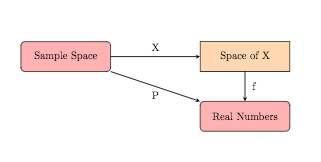
\includegraphics[width=1\linewidth]{images/randomvariable.png}
\par
We will make various restrictions on the range of the random variable to fit different 
	generalized problems. Then, we will be able to work on a problem (which may be 
	inherently non-numerical) by using the random variable in subsequent calculations.
	%
\begin{example}[Success vs Failure]\label{example-10}
When dealing with only two outcomes, one might use 
	\begin{equation*}S = \text{{ success, failure }}.\end{equation*}
	Choose 
	\begin{gather*}
X(success)=1\\
X(failure)=0.
\end{gather*}
	Then, R={0,1}.
	%
\end{example}
\begin{example}[Standard Dice Pairs]\label{example-11}
When gambling with a pair of dice, one might use
	S=ordered pairs of all possible rolls.  Then 
	\begin{equation*}S = \text{ {(a,b): a=die 1 outcome, b=die 2 outcome}}.\end{equation*}
	Choose 
	\begin{equation*}X( (a,b) ) = a+b.\end{equation*} 
	Then, R={2, 3, 4, 5, ..., 12}.
	%
\end{example}
\begin{example}[Other Dice Options]\label{example-12}
When rolling dice in a board game (like RISK), one might use
	\begin{equation*}S= \text{{(a,b): a=die 1 outcome, b=die 2 outcome}}\end{equation*}
	Choose 
	\begin{equation*}X( (a,b) ) = \text{max{a,b}}.\end{equation*} 
	Then, R={1, 2, 3, 4, 5, 6}.
	%
\end{example}
\begin{definition}[{}]\label{definition-22}

		R contains a countable number of points if either R is finite or there 
		is a one to one correspondence between R and the positive integers. 
		Such a set will be called discrete. We will see that often the set R is not countable. 
		If R consists of an interval of points (or a union of intervals), 
		then we call X a continuous random variable. 
		\end{definition}
\typeout{************************************************}
\typeout{Subsection 5.2.1 HOMEWORK}
\typeout{************************************************}
\subsection[{HOMEWORK}]{HOMEWORK}\label{subsection-2}

	A. You flip three coins and measure the number of heads obtained. Determine the space R for the corresponding random variable X. From the eight possible outcomes, determine all outcomes corresponding to X=2. Identify the random variable as discrete or continuous.
	%
\par

	B. You flip one coin repeatedly until you get a second head. Determine the space R for the corresponding random variable X. From the possibilities, determine all outcomes corresponding to X=4. Identify the random variable as discrete or continuous.
	%
\par

	C. Now you want to measure the time between accidents at a particular intersection in town. Determine the space R for the corresponding random variable X. Describe all outcomes corresponding to \(X \lt 1\). Be purposeful in the problem to describe the units you are using to measure time. Identify the random variable as discrete or continuous.
	%
\typeout{************************************************}
\typeout{Section 5.3 Probability Functions}
\typeout{************************************************}
\section[{Probability Functions}]{Probability Functions}\label{section-26}
In the formulas below, we will presume that we have a random variable X which maps the sample space S onto some range of real numbers R.  From this set, we then can define a probability function f(x) which acts on the numerical values in R and returns another real number.  We attempt to do so to obtain (for discrete values) P(sample space value s)\( = f(X(s))\).  That is, the probability of a given outcome s is equal to the composition which takes s to a numerical value x which is then plugged into f to get the same final values.%
\begin{definition}[{Probability "Mass" Function}]\label{definition-23}
Given a discrete random variable X on a space R, a probability mass function on X is given by a function \(f:R \rightarrow \mathbb{R}\) such that:
		\begin{align*}
& \forall x \in R , f(x) \gt 0\\
& \sum_{x \in R} f(x) = 1\\
& A \subset R \Rightarrow P(X \in A) = \sum_{x \in A}f(x)
\end{align*}
		For \(x \not\in R\), you can use the convention f(x)=0.
		\end{definition}
\begin{definition}[{Probability "Density" Function}]\label{definition-24}
Given a continuous random variable X on a space R, a probability density function on X is given by a function \(f:R \rightarrow \mathbb{R}\) such that:
			\begin{align*}
& \forall x \in R , f(x) \gt 0\\
& \int_{R} f(x) dx = 1\\
& A \subset R \Rightarrow P(X \in A) = \int_{A} f(x) dx
\end{align*}
		For \(x \not\in R\), you can use the convention f(x)=0.
		\end{definition}
\par

	For the purposes of this book, we will use the term "Probability Function" to refer to either of these options.
	%
\begin{example}[Discrete Probability Function]\label{example-13}

	Consider \(f(x) = x/10\) over R = {1,2,3,4}.  Then, f(x) is obviously positive for each of the values in R and certainly \(\sum_{x \in R} f(x) = f(1) + f(2) + f(3) + f(4) = 1/10 + 2/10 + 3/10 + 4/10 = 1\). Therefore, f(x) is a probability mass function over the space R.
	%
\end{example}
\begin{lstlisting}[style=sageinput]
# Combining all of the above into one interactive cell
@interact
def _(D = input_box([1,2,3,5,6,8,9,11,12,14],label="Enter domain R (in brackets):"), 
       Probs = input_box([1/20,1/20,1/20,3/20,1/20,4/20,4/20,1/20,1/20,3/20],label="Enter corresponding f(x) (in brackets):"),
       n_samples=slider(100,10000,100,100,label="Number of times to sample from this distribution:")):
    n = len(D)
    R = range(n)
    one_huh = sum(Probs)
    pretty_print('\n\nJust to be certain, we should check to make certain the probabilities sum to 1\n')
    pretty_print(html('$\sum_{x\epsilon R} f(x) = %s$'%str(one_huh)))
    
    G = Graphics()
    if len(D)==len(Probs):
        f = zip(D,Probs)
        meanf = 0
        variancef = 0
        for k in R:
            meanf += D[k]*Probs[k]
            variancef += D[k]^2*Probs[k]
            G += line([(D[k],0),(D[k],Probs[k])],color='green')
        variancef = variancef - meanf^2
        sd = sqrt(variancef)
        G += points(f,color='blue',size=50)
        G += point((meanf,0),color='yellow',size=60,zorder=3)
        G += line([(meanf-sd,0),(meanf+sd,0)],color='red',thickness=5)
    
        g = DiscreteProbabilitySpace(D,Probs)
        pretty_print('     mean = %s'%str(meanf))
        pretty_print(' variance = %s'%str(variancef))
    
        #  perhaps to add mean and variance for pmf here
    else:
        print 'Domain D and Probabilities Probs must be lists of the same size'
    
    #  Now, let's sample from the distribution given above and see how a random sampling matches up

    counts = [0] * len(Probs)
    X = GeneralDiscreteDistribution(Probs)
    sample = []

    for _ in range(n_samples):
        elem = X.get_random_element()
        sample.append(D[elem])
        counts[elem] += 1
    Empirical = [1.0*x/n_samples for x in counts] # random
    
    samplemean = mean(sample)
    samplevariance = variance(sample)
    sampdev = sqrt(samplevariance)
    
    E = points(zip(D,Empirical),color='orange',size=40)
    E += point((samplemean,0.005),color='brown',size=60,zorder=3)
    E += line([(samplemean-sampdev,0.005),(samplemean+sampdev,0.005)],color='orange',thickness=5)    
    (G+E).show(ymin=0,figsize=(8,5))
\end{lstlisting}
\begin{example}[Continuous Probability Function]\label{example-14}

	Consider \(f(x) = x^2/c\) for some positive real number c and presume R = [-1,2]. Then f(x) is nonnegative (and only equals zero at one point). To make f(x) a probability density function, we must have
	\begin{equation*}\int_{x \in R} f(x) = 1.\end{equation*}
	In this instance you get
	\begin{equation*}1 = \int_{-1}^2 x^2/c = x^3/(3c) |_{-1}^2 = \frac{8}{3c} - \frac{-1}{3c} = \frac{3}{c}\end{equation*}
	Therefore, f(x) is a probability density function over R provided   = 3.
	%
\end{example}
\begin{definition}[{Distribution Function}]\label{definition-25}
Given a random variable X on a space R, a probability distribution function on X is given by a function 
				   \(F:\mathbb{R} \rightarrow \mathbb{R}\) such that \(\displaystyle F(x)=P(X \le x)\)\end{definition}
\begin{example}[Discrete Distribution Function]\label{example-15}
Using \(f(x) = x/10\) over R = {1,2,3,4} again, note that F(x) will only change at these four domain values. We get
	
	\leavevmode%
\begin{table}
\centering
\begin{tabular}{rr}
\multicolumn{1}{rB}{X}&F(x)\tabularnewline\hrulemedium
\multicolumn{1}{rB}{\(x \lt 1\)}&0\tabularnewline[0pt]
\multicolumn{1}{rB}{\(1 \le x \lt 2\)}&1/10\tabularnewline[0pt]
\multicolumn{1}{rB}{\(2 \le x \lt 3\)}&3/10\tabularnewline[0pt]
\multicolumn{1}{rB}{\(3 \le x \lt 4\)}&6/10\tabularnewline[0pt]
\multicolumn{1}{rB}{\(4 \le x \)}&1
\end{tabular}
\end{table}

	%
\end{example}
\begin{example}[Continuous Distribution Function]\label{example-16}

	Consider \(f(x) = x^2/3\) over R = [-1,2].  Then, for \(-1 \le x \le 2\),
	\begin{equation*}F(x) = \int_{-1}^x u^2/3 du = x^3/9 + 1/9.\end{equation*}
	Notice, F(-1) = 0 since nothing has yet been accumulated over values smaller than -1 and F(2)=1 since by that time everything has been accumulated. In summary:
	
	\leavevmode%
\begin{table}
\centering
\begin{tabular}{rr}
\multicolumn{1}{rB}{X}&F(x)\tabularnewline\hrulemedium
\multicolumn{1}{rB}{\(x \lt -1\)}&0\tabularnewline[0pt]
\multicolumn{1}{rB}{\(-1 \le x \lt 2\)}&\(x^3/9 + 1/9\)\tabularnewline[0pt]
\multicolumn{1}{rB}{\(2 \le x\)}&1
\end{tabular}
\end{table}

	
	
	%
\end{example}
\begin{theorem}[{}]\label{theorem-Fmin}
\(F(x)=0, \forall x \lt \inf(R)\)\end{theorem}
\begin{proof}\hypertarget{proof-21}{}

		Let a = inf(R). Then, for 
		\begin{equation*}x \lt a, F(x) = P(X \le x) \le P(X \lt a) = 0\end{equation*} 
		since none of the x-values in this range are in R.
		%
\end{proof}
\begin{theorem}[{}]\label{theorem-Fmax}
\(F(x)=1, \forall x \ge \sup(R)\)\end{theorem}
\begin{proof}\hypertarget{proof-22}{}

		Let b = sup(R). Then, for 
		\begin{equation*}x \ge b, F(x) = P(X \le x)  = P(X \le b) + P( b \lt X le x) = P(X le b) = 1\end{equation*} 
		since all of the x-values in this range are in R and therefore will either sum over or integrate over all of R.
		%
\end{proof}
\begin{theorem}[{}]\label{theorem-22}
F is non-decreasing\end{theorem}
\begin{proof}\hypertarget{proof-23}{}
Case 1: R discrete%
\begin{align*}
\forall x_1,x_2 \in \mathbb{Z} \ni x_1 \lt x_2\\
F(x_2) & = \sum_{x \le x_2} f(x) \\
& = \sum_{x \le x_1} f(x) + \sum_{x_1 \lt x \le x_2} f(x)\\
& \ge \sum_{x \le x_1} f(x) = F(x_1)
\end{align*}\par
Case 2: R continuous%
\begin{align*}
\forall x_1,x_2 \in \mathbb{R} \ni x_1 \lt x_2\\
F(x_2) & = \int_{-\infty}^{x_2} f(x) dx \\
 & = \int_{-\infty}^{x_1} f(x) dx + \int_{x_1}^{x_2} f(x) dx\\
 & \ge \int_{-\infty}^{x_1} f(x) dx\\
 & = F(x_1)
\end{align*}\end{proof}
\begin{theorem}[{Using Discrete Distribution Function to compute probabilities}]\label{theorem-Fvsf-discrete}
for \(x \in R, f(x) = F(x) - F(x-1)\)\end{theorem}
\begin{proof}\hypertarget{proof-24}{}
Assume \(x \in R\) for some discrete R. Then,
		\begin{equation*}F(x) - F(x-1) = \sum_{u \le x} f(u) - \sum_{u \lt x} f(u) = f(x)\end{equation*}
		%
\end{proof}
\begin{theorem}[{Using Continuous Distribution function to compute probabilities}]\label{theorem-Fvsf-continuyous}
for \(a \lt b, (a,b) \in R, P(a \lt X \le b) = F(b) - F(a)\)\end{theorem}
\begin{proof}\hypertarget{proof-25}{}

		For a and b as noted, consider 
		\begin{align*}
F(b) - F(a) & = \int_{-\infty}^b f(x) dx - \int_{-\infty}^a f(x) dx\\
 & = \int_a^b f(x) dx \\
 & = P(a \lt x \le b)
\end{align*}
		%
\end{proof}
\begin{corollary}[{}]\label{corollary-ProbPointZero-continuous}
For continuous distributions, P(X = a) = 0\end{corollary}
\begin{proof}\hypertarget{proof-26}{}

		We will assume that F(x) is a continuous function. With that assumption, note
		\begin{equation*}P(a-\epsilon \lt  x \le a)  = \int_{a-\epsilon}^a f(x) dx = F(a) - F(a-\epsilon)\end{equation*}
		Take the limit as \( \epsilon \rightarrow 0^+\) to get the result noting that
		%
\end{proof}
\begin{theorem}[{F(x) vs f(x), for continuous distributions}]\label{theorem-25}
If X is a continuous random variable, f the corresponding probability function, and F the associated distribution function, then
			\begin{equation*}f(x) = F'(x)\end{equation*}
		%
\end{theorem}
\begin{proof}\hypertarget{proof-27}{}
Assume X is continuous and f and F as above. Notice, by the definition of f, \(\lim_{x \rightarrow \pm \infty} f(x) = 0\) since otherwise the integral over the entire space could not be finite.
	%
\par

	Now, let A(x) be any antiderivative of f(x). Then, by the Fundamental Theorem of Calculus,
	\begin{align*}
F(x) & = \int_{-\infty}^x f(u) du\\
 & = A(x) - \lim_{u \rightarrow -\infty} A(u)
\end{align*}
	Hence, \(F'(x) = A'(x) - \lim_{u \rightarrow -\infty} A'(u) = f(x)\) as desired.
	%
\end{proof}
\typeout{************************************************}
\typeout{Subsection 5.3.1 HOMEWORK}
\typeout{************************************************}
\subsection[{HOMEWORK}]{HOMEWORK}\label{subsection-3}

	A.  Consider the random variable from the previous section where you flip three coins and measure the number of heads obtained. Determine f(0), f(1), f(2), and f(3) and the corresponding distribution function F(x). These can be expressed in a table format. Generalize your answer to the case when you flip a n coins where n is a fixed natural number.
	%
\par

	B.  
	%
\typeout{************************************************}
\typeout{Section 5.4 Expected Value}
\typeout{************************************************}
\section[{Expected Value}]{Expected Value}\label{section-27}
Blaise Pascal was a 	17th century mathematician and philosopher who was accomplished in many areas but may likely be best known to you for his creation of what is now known as Pascal's Triangle. As part of his philosophical pursuits, he proposed what is known as "Pascal's wager". It suggests two  mutually exclusive outcomes: that God exists or that he does not. His argument is that a rational person should live as though God exists and seek to believe in God. If God does not actually exist, such a person will have only a finite loss (some pleasures, luxury, etc.), whereas they stand to receive infinite gains as represented by eternity in Heaven and avoid an infinite losses of eternity in Hell. This type of reasoning is part of what is known as "decision theory".
	%
\par
You may not confront such dire payouts when making your daily decisions but we need a formal method for making these determinations precise. The procedure for doing so is what we call expected value.
	%
\begin{definition}[{Expected Value}]\label{definition-26}
Given a random variable X over space R, corresponding probability function f(x) and "value function" u(x), the expected value of u(x) is given by
	\begin{equation*}E = E[u(X)] = \sum_{x \in R} u(x) f(x)\end{equation*}
	provided X is discrete, or
	\begin{equation*}E = E[u(X)] = \int_R u(x)f(x) dx\end{equation*}
	provided X is continuous.
	%
\end{definition}
\begin{theorem}[{Expected Value is a Linear Operator}]\label{theorem-26}

	\leavevmode%
\begin{enumerate}
\item\hypertarget{li-156}{}E[c] = c%
\item\hypertarget{li-157}{}E[c u(X)] = c E[u(X)]%
\item\hypertarget{li-158}{}E[u(X) + v(X)] = E[u(X)] + E[v(X)]%
\end{enumerate}

	%
\end{theorem}
\begin{proof}\hypertarget{proof-28}{}
Each of these follows by utilizing the corresponding linearity properties of the summation and integration operations. For example, to verify part three in the continuous case:
	\begin{align*}
E[u(X) + v(X)] & = \int_{x \in R} [u(x)+v(x)]f(x) dx\\
 & = \int_{x \in R} u(x)f(x) dx + \int_{x \in R} u(x)f(x) dx\\
 & = E[u(X)] + E[v(X)].
\end{align*}
	%
\end{proof}
\begin{example}[Discrete Expected Value]\label{example-17}
Consider \(f(x) = x/10\) over R = {1,2,3,4} where the payout is 10 euros if x=1, 5 euros if x=2, 2 euros if x=3 and -7 euros if x = 4.  Then your value function would be u(1)=10, u(2) = 5, u(3)=2, and u(4) = -7. Computing the expect payout gives
	\begin{equation*}E = 10 \times 1/10 + 5 \times 2/10 + 2 \times 3/10 - 7 \times 4/10 = -2/10\end{equation*}
	Therefore, the expected payout is actually negative due to a relatively large negative payout associated with the largest likelihood outcome and the larger positive payout only associated with the least likely outcome.
	%
\end{example}
\begin{example}[Continuous Expected Value]\label{example-18}

	Consider \(f(x) = x^2/3\) over R = [-1,2] with value function given by \(u(x) = e^x - 1\). Then, the expected value for u(x) is given by
	\begin{equation*}E = \int_{-1}^2 (e^x-1) \cdot x^2/3 = -1/9 \cdot (e + 15) \cdot e^{-1} + 2/3 \cdot e^2 - 8/9 \approx 3.3129\end{equation*}
	%
\end{example}
\begin{definition}[{Theoretical Measures}]\label{definition-27}

	Given a random variable with probability function f(x) over space R
	\leavevmode%
\begin{enumerate}
\item\hypertarget{li-159}{}The mean of X = \(\mu = E[x]\)%
\item\hypertarget{li-160}{}The variance of X = \(\sigma^2 = E[(x-\mu)^2]\)%
\item\hypertarget{li-161}{}The skewness of X = \(\gamma_1 = \frac{E[(x-\mu)^3]}{\sigma^3}\)%
\item\hypertarget{li-162}{}The kurtosis of X = \(\gamma_2 = \frac{E[(x-\mu)^4]}{\sigma^4}\)%
\end{enumerate}

	%
\end{definition}
\begin{theorem}[{Alternate Formulas for Theoretical Measures}]\label{theorem-27}

	\leavevmode%
\begin{enumerate}
\item\hypertarget{li-163}{}\(\sigma^2 = E[x^2] - \mu^2 = E[X(x-1)] + \mu - \mu^2\)%
\item\hypertarget{li-164}{}\(\gamma_1 = \frac{1}{\sigma^3} \cdot \left [ E[X^3] - 3 \mu E[X^2] + 2\mu^3 \right ]\)%
\item\hypertarget{li-165}{}\(\gamma_2 = \frac{1}{\sigma^4} \cdot \left [ E[X^4] - 4 \mu E[X^3] + 6\mu^2 E[X^2] - 3 \mu^4 \right ]\)%
\end{enumerate}

	%
\end{theorem}
\begin{proof}\hypertarget{proof-29}{}

		In each case, expand the binomial inside and use the linearity of expected value.
		%
\end{proof}
\par

	Consider the following example when computing these statistics for a discrete variable. In this case, we will utilize a variable with a relatively small space so that the summations can be easily done by hand. Indeed, consider
	
	\leavevmode%
\begin{table}
\centering
\begin{tabular}{rr}
\multicolumn{1}{rB}{X}&f(x)\tabularnewline\hrulemedium
\multicolumn{1}{rB}{0}&0.10\tabularnewline[0pt]
\multicolumn{1}{rB}{1}&0.25\tabularnewline[0pt]
\multicolumn{1}{rB}{2}&0.40\tabularnewline[0pt]
\multicolumn{1}{rB}{4}&0.15\tabularnewline[0pt]
\multicolumn{1}{rB}{7}&0.10
\end{tabular}
\end{table}

	
	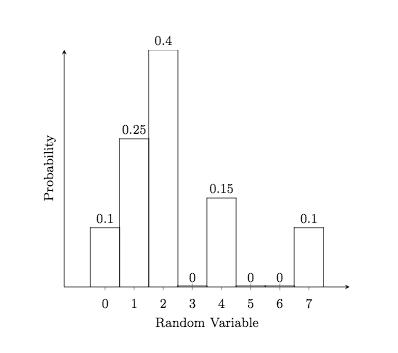
\includegraphics[width=1\linewidth]{images/DiscreteHistogramExample.png}

	%
\par

	Using the definition of mean as a sum,
	\begin{align*}
\mu & = 0 \cdot 0.10 + 1 \cdot 0.25 + 2 \cdot 0.40 + 4 \cdot 0.15 + 7 \cdot 0.10\\
 & = 0 + 0.25 + 0.80 + 0.60 + 0.70\\
 & = 2.35
\end{align*}
	Notice where this lies on the probability histogram for this distribution.
	%
\par
For the variance
	\begin{align*}
\sigma^2 & = E[X^2] - \mu^2\\
 & = \left [ 0^2 \cdot 0.10 + 1^2 \cdot 0.25 + 2^2 \cdot 0.40 + 4^2 \cdot 0.15 + 7^2 \cdot 0.10 \right ] - 2.35^2\\
 & = 0 + 0.25 + 1.60 + 2.40 + 4.90 - 5.5225\\
 & = 9.15 - 5.225\\
 & = 3.6275 
\end{align*}	
	and so the standard deviation \(\sigma = \sqrt{3.6275} \approx 1.90\). Notice that 4 times this value encompasses almost all of the range of the distribution.
	%
\par
For the skewness
	\begin{align*}
 \text{Numerator = } & E[X^3] - 3 \mu E[X^2] + 2\mu^3\\
 & = \left [ 0^3 \cdot 0.10 + 1^3 \cdot 0.25 + 2^3 \cdot 0.40 + 4^3 \cdot 0.15 + 7^3 \cdot 0.10 \right ] - 3 \cdot 2.35 \cdot 9.15 + 2 \cdot 2.35^3\\
 & \approx 0 + 0.25 + 3.20 + 9.60 + 34.3 - 64.5075 + 25.96\\
 & = 47.35 - 64.5075 + 25.96\\
 & \approx 8.80
\end{align*}
	which yields a skewness of \(\gamma_1 = 8.80 / \sigma^3 \approx 1.27 \). This indicates a slight skewness to the right of the mean. You can notice the 4 and 7 entries on the histogram illustrate a slight trailing off to the right.
	%
\par
Finally, for kurtosis
	\begin{align*}
 \text{Numerator = } & E[X^4] - 4 \mu E[X^3] + 6 \mu^2 E[X^2] - 3\mu^4\\
 & = \left [ 0^4 \cdot 0.10 + 1^4 \cdot 0.25 + 2^4 \cdot 0.40 + 4^4 \cdot 0.15 + 7^4 \cdot 0.10 \right ] - 4 \cdot 2.35 \cdot 47.35 + 6 \cdot 2.35^2 \cdot 9.15^2 - 3 \cdot 2.35^4\\
 & \approx 0 + 0.25 + 6.40 + 38.4 + 240.1 - 445.09 + 303.19 - 91.49\\
 & \approx 285.15 - 445.09 + 303.19 - 91.49\\
 & \approx 51.75
\end{align*}
	which yields a kurtosis of \(\gamma_2 = 51.75 / \sigma^4 \approx 3.93\) which also notes that the data appears to have a modestly bell-shaped distribution.
	%
\par

	Consider the following example when computing these statistics for a continuous variable. 
	Let \(f(x) = \frac{3}{4} \cdot (1-x^2)\) over R = [-1,1].  
		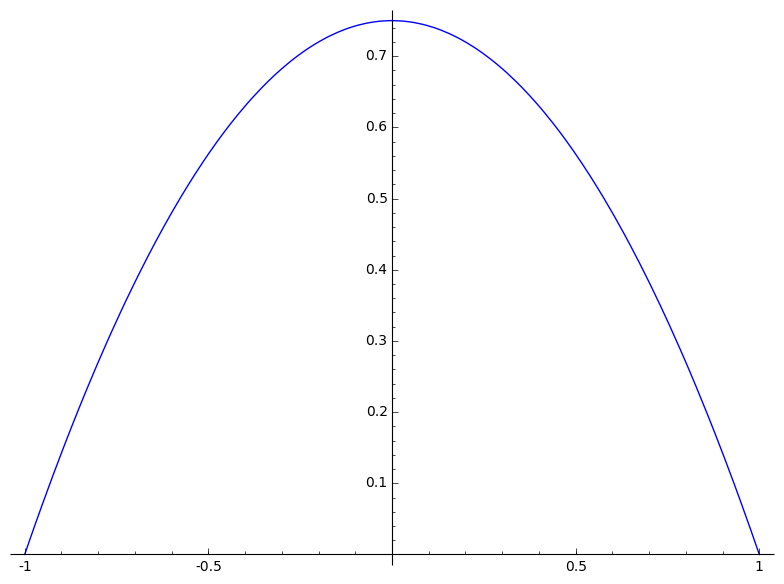
\includegraphics[width=1\linewidth]{images/ContinuousDistributionExample.png}

	%
\par

	Then for the mean
	\begin{align*}
\mu & = \int_{-1}^1 x \cdot \frac{3}{4} \cdot (1-x^2) dx\\
 & = \int_{-1}^1 \frac{3}{4} \cdot (x-x^3) dx\\
 & = \frac{3}{4} \cdot (x^2/2-x^4/4) \big |_{-1}^1\\
 & = \frac{3}{4} \cdot [(1/2)-(1/4)] - [(1/2) - (1/4)]\\
 & = 0
\end{align*}
	as expected since the probability function is symmetric about x=0.
	%
\par
For the variance
	\begin{align*}
\sigma^2 & = \int_{-1}^1 x^2 \cdot \frac{3}{4} \cdot (1-x^2) dx - \mu^2\\
 & = \int_{-1}^1 \cdot \frac{3}{4} \cdot (x^2-x^4) dx - 0\\
 & = \frac{3}{4} \cdot (x^3 /3 -x^5 / 5) \big |_{-1}^1\\
 & = \frac{3}{4} \cdot 2 \cdot (1/3-1/5)\\
 & = \frac{3}{4} \cdot \frac{4}{15}\\
 & = \frac{1}{5}
\end{align*}
	and taking the square root gives a standard deviation slightly less than 1/2. Notice that four times this value encompasses almost all of the range of the distribution.
	%
\par
For the skewness, notice that the graph is symmetrical about the mean and so we would expect a skewness of 0.  Just to check it out
	\begin{align*}
 \text{Numerator = } & E[X^3] - 3 \mu E[X^2] + 2\mu^3\\
 & = \int_{-1}^1 x^3 \cdot \frac{3}{4} \cdot (1-x^2) dx - 3 E[X^2] \cdot 0 + 0^3 \\
 & = \int_{-1}^1 \cdot \frac{3}{4} \cdot (x^3-x^5) dx\\
 & = \frac{3}{4} \cdot (x^4/4-x^6/6) \big |_{-1}^1\\
 & = 0
\end{align*}
	as expected without having to actually complete the calculation by dividing by the cube of the standard deviation.
	%
\par
Finally, note that the probability function in this case is modestly close to a bell shaped curve so we would expect a kurtosis in the vicinity of 3. Indeed, noting that (conveniently) \(\mu = 0\) gives
	\begin{align*}
 \text{Numerator = } & E[X^4] - 4 \mu E[X^3] + 6 \mu^2 E[X^2] - 3 \mu^4\\
 & = \int_{-1}^1 x^4 \cdot \frac{3}{4} \cdot (1-x^2) dx\\
 & = \frac{3}{4} \cdot (x^5 /5-x^7 /7) \big |_{-1}^1\\
 & = \frac{3}{4} \cdot 2(1/5-1/7)\\
 & = \frac{3}{35}
\end{align*}
	and so by dividing by \(\sigma^4 = \sqrt{\frac{1}{5}}^4 = \frac{1}{25}\) gives a kurtosis of
	\begin{equation*}\gamma_2 = \frac{3}{35} / \frac{1}{25} = \frac{75}{35} \approx 2.14.\end{equation*}
	%
\begin{example}[Roulette]\label{example-19}

Roulette is a gambling game popular in may casinos in which a player attempts to win money from the casino by predicting the location that a ball lands on in a spinning wheel.  There are two variations of this game...the American version and the European version. The difference being that the American version has one additional numbered slot on the wheel. The American version of the game will be used for the purposes of this example.
%
\par

A Roulette wheel consists of 38 equally-sized sectors identified with the numbers 1 through 36 plus 0 and 00. The 0 and 00 sectors are colored green and half of the remaining numbers are in sectors colored red with the remainder colored black.  A steel ball is dropped onto a spinning wheel and as the wheel comes to rest the sector in which it comes to rest is noted.  It is easy to determine that the probability of landing on any one of the 38 sectors is 1/38. A picture of a typical American-style wheel and betting board is given by
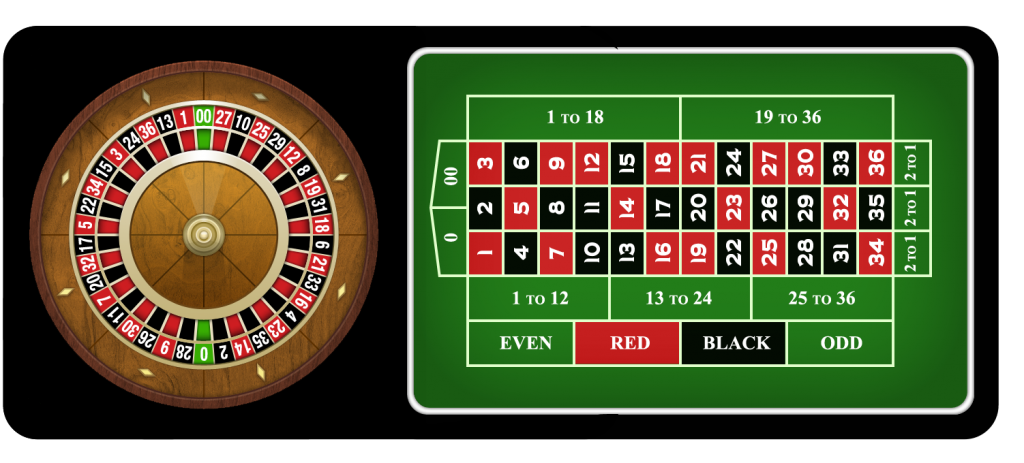
\includegraphics[width=1\linewidth]{images/6-1-American-Roulette-1024x463.png}
. (Found at BigFishGames.com.)
%
\par

Since this is a game in a casino, there must be the opportunity to bet (and likely lose) money. For the remainder of this example we will assume that you are betting 1 dollar each time. If you were to bet more then the values would scale correspondingly. However, if you place your bet on any single number and the ball ends up on the sector corresponding to that number, you win a net of 35 dollars.  If the ball lands elsewhere you lose your dollar. Therefore the expected value of winning if you bet on one number is
\begin{equation*}E[\text{win on one}] = 35 \cdot \frac{1}{38} - 1 \cdot \frac{37}{38} = - \frac{2}{38}\end{equation*}
which is a little more than a nickel loss on average.
%
\par

You can bet on two numbers as well and if the ball lands on either of the two then you win a payout in this case of 17 dollars.  Therefore the expected value of winning if you bet on two numbers is
\begin{equation*}E[\text{win on two numbers}] = 17 \cdot \frac{2}{38} - 1 \cdot \frac{36}{38} = - \frac{2}{38}.\end{equation*}
%
\par

Continuing, you can bet on three numbers and if the ball lands on any of the three then you win a payout of 11 dollars.  Therefore the expected value of winning if you bet on three numbers is
\begin{equation*}E[\text{win on three numbers}] = 11 \cdot \frac{3}{38} - 1 \cdot \frac{35}{38} = - \frac{2}{38}.\end{equation*}
%
\par

You can bet on all reds, all blacks, all evens (ignoring 0 and 00), or all odds and get your dollar back. The expected value for any of these options is
\begin{equation*}E[\text{win on eighteen numbers}] = 1 \cdot \frac{18}{38} - 1 \cdot \frac{20}{38} = - \frac{2}{38}.\end{equation*}
%
\par
There is one special way to bet which uses the the 5 numbers {0, 00, 1, 2, 3} and pays 6 dollars. This is called the "top line of basket".  Notice that the use of five numbers will make getting the same expected value as the other cases impossible using regular dollars and cents. The expected value of winning in this case us
\begin{equation*}E[\text{win on top line of basket}] = 6 \cdot \frac{5}{38} - 1 \cdot \frac{33}{38} = - \frac{3}{38}\end{equation*}
which is of course worse and is the only normal way to bet on roulette which has a different expected value. 
%
\par

There are other possible ways to bet on roulette but none provide a better expected value of winning.  The moral of this story is that you should never bet on the 5 number option and if you ever get ahead by winning on roulette using any of the possible options then you should probably stop quickly since over a long period of time it is expected that you will lose an average of \(\frac{1}{19}\) dollars per game.
%
\end{example}
\par
Going back to Pascal's wager, let X = 0 represent disbelief when God doesn't exist and X = 1 represent disbelief when God does exist, X = 2 represent belief when God does exist, and X = 3 represent belief when God does not exist. Let p be the likelihood that God exists. Then you can compute the expected value of disbelief and the expect value of belief by first creating a value function. Below, for argument sake we are somewhat randomly assign a value of one million to disbelief if God doesn't exist. The conclusions are the same if you choose any other finite number...
	\begin{gather*}
u(0) = 1,000,000, f(0) = 1-p\\
u(1) = -\infty, f(1) = p\\
u(2) = \infty, f(2) = p\\
u(3) = 0, f(3) = 1-p
\end{gather*}
	Then, 
	\begin{align*}
E[\text{disbelief}] & = u(0)f(0) + u(1)f(1)\\
& = 1000000 \times (1-p) - \infty \times p\\
& = -\infty
\end{align*}
	if p>0. On the other hand, 
	\begin{align*}
E[\text{belief}] & = u(2)f(2) + u(3)f(3)\\
& = \infty \times p + 0 \times (1-p)\\
& = \infty
\end{align*}
	if p>0. So Pascal's conclusion is that if there is even the slightest chance that God exists then belief is the smart and scientific choice.
	%
\typeout{************************************************}
\typeout{Section 5.5 Standard Units}
\typeout{************************************************}
\section[{Standard Units}]{Standard Units}\label{section-28}
Any distribution variable can be converted to “standard units” using the linear translation 
	\(\displaystyle z = \frac{x-\mu}{\sigma}\). In doing so, then values of z will always represent the number of
	standard deviations x is from the mean and will provide “dimensionless” comparisons.%
\typeout{************************************************}
\typeout{Chapter 6 Distributions based upon Equally likely Outcomes}
\typeout{************************************************}
\chapter[{Distributions based upon Equally likely Outcomes}]{Distributions based upon Equally likely Outcomes}\label{UniformHypergeometric}
\typeout{************************************************}
\typeout{Section 6.1 Introduction}
\typeout{************************************************}
\section[{Introduction}]{Introduction}\label{section-29}

	When motivating our definition of probability you may have noticed that we modeled our definition on the relative frequency of equally-likely outcomes. In this chapter you will develop the theoretical formulas which can be used to model equally-likely outcomes.
	%
\par

In this chapter, you will investigate the following distributions:
\leavevmode%
\begin{enumerate}
\item\hypertarget{li-166}{}Discrete Uniform - each of a finite collection of outcomes is equally likely and prescribed a "position" and X measures the position of an item selected randomly from the outcomes.%
\item\hypertarget{li-167}{}Continuous Uniform - an interval of values is possible with sub-intervals of equal length having equal probabilities and X measures a location inside that interval.%
\item\hypertarget{li-168}{}Hypergeometric - each of a finite collection of values are equally likely and grouped into two classes (successes vs failures) and a subset of that collection is extracted with X measuring the number of successes in the sample.%
\end{enumerate}

%
\typeout{************************************************}
\typeout{Section 6.2 Discrete Uniform Distribution}
\typeout{************************************************}
\section[{Discrete Uniform Distribution}]{Discrete Uniform Distribution}\label{section-30}

	Assume that you have a variable with space R = {1, 2, 3, ..., n} so that the likelihood of each value is equally likely. Then, the probability function satisfies \(f(x) = c\) for any \(x \in R\).  As before, since \(\sum_{x \in R} f(x) = 1\), then \begin{equation*}f(x) = \frac{1}{n}\end{equation*} is the probability function.
	%
\begin{lstlisting}[style=sageinput]
# Uniform distribution over 1 .. n
pretty_print("Discrete Uniform Distribution over the set 1, 2, ..., n")
var('x')
@interact
def _(n=slider(2,10,1,2)):
    np1 = n+1
    R = range(1,np1)
    f(x) = 1/n
    pretty_print(html('Density Function: $f(x) =%s$'%str(latex(f(x)))+' over the space $R = %s$'%str(R)))
    points((k,f(x=k)) for k in R).show()
    for k in R:
        pretty_print(html('$f(%s'%k+') = %s'%f(x=k)+' \\approx %s$'%f(x=k).n(digits=5)))
\end{lstlisting}
\begin{theorem}[{Properties of the Discrete Uniform Probability Function}]\label{theorem-28}
\leavevmode%
\begin{enumerate}
\item\hypertarget{li-169}{}\(f(x) = \frac{1}{n}\) over R = {1, 2, 3, ..., n} satisfies the properties of a discrete probability function%
\item\hypertarget{li-170}{}\(\mu = \frac{1+n}{2}\)%
\item\hypertarget{li-171}{}\(\sigma^2 = \frac{n^2-1}{12}\)%
\item\hypertarget{li-172}{}\(\gamma_1 = 0\)%
\item\hypertarget{li-173}{}\(\gamma_2 = \frac{6}{5}\frac{1+n^2}{1-n^2}\)%
\item\hypertarget{li-174}{}Distribution function F(x) = frac{x}{n} for \(x \in R\).%
\end{enumerate}
\end{theorem}
\begin{proof}\hypertarget{proof-30}{}
\leavevmode%
\begin{enumerate}
\item\hypertarget{li-175}{}Trivially, by construction you get \begin{equation*}\sum_{k=1}^n \frac{1}{n} = 1\end{equation*}
		Also, 1/n is positive for all x values.
		%
\item\hypertarget{li-176}{}To determine the mean,
		\begin{align*}
\mu & = \sum_{k=1}^n x \cdot \frac{1}{n}\\
 & = \frac{1}{n}\sum_{k=1}^n x \\
 & = \frac{1}{n} \frac{n(n+1)}{2}\\
 & = \frac{1+n}{2}
\end{align*}
		%
\item\hypertarget{li-177}{}To determine the variance,
		\begin{align*}
\sigma^2 & = \sum_{k=1}^n x^2 \cdot \frac{1}{n} - \mu^2\\
 & = \frac{1}{n}\sum_{k=1}^n x^2 - \left ( \frac{1+n}{2}\right )^2 \\
 & = \frac{1}{n} \frac{n(n+1)(2n+1)}{6} - \frac{1+2n+n^2}{4}\\
 & = \frac{(2n^2+3n+1)}{6} - \frac{1+2n+n^2}{4}\\
 & = \frac{(4n^2+6n+2)}{12} - \frac{3+6n+3n^2}{12}\\
 & = \frac{(n^2-1)}{12}
\end{align*}
		%
\item\hypertarget{li-178}{}For skewness,
		\begin{align*}
\gamma_1 = & \sum_{k=1}^n x^3 \cdot \frac{1}{n} - 3 \mu \sum_{k=1}^n x^2 \cdot \frac{1}{n}  + 2\mu^3\\
 & = \frac{n^2(n+1)^2}{4n} - 3\frac{(n(n+1))}{2} \frac{1+n}{2} + 2 \left ( \frac{1+n}{2}\right )^3 \\
 & = 
\end{align*}
		%
\item\hypertarget{li-179}{}For Kurtosis, use the fourth moment and simplify...the algebra is performed using Sage in the active cell below this proof.
		%
\item\hypertarget{li-180}{}

		%
\end{enumerate}
\end{proof}
\par

	Sage can also do the algebra for you to determine each of these measures. Notice, as n increases the Kurtosis approaches \(\frac{6}{5}\) which indicates that there is (obviously) no tend toward central tendency over time.
	%
\begin{lstlisting}[style=sageinput]
var('x,n')
f = 1/n
mu = sum(x*f,x,1,n).factor()
pretty_print('Mean = ',mu)
mu = (1+n)/2
v = sum((x-mu)^2*f, x, 1, n)
pretty_print('Variance = ',v.factor())
stand = sqrt(v)
pretty_print('Skewness =  ',(sum((x-mu)^3*f, x, 1, n)/stand^3))
kurt = sum((x-mu)^4*f, x, 1, n)/stand^4
pretty_print('Kurtosis = ',(kurt-3).factor(),' + 3')
\end{lstlisting}
\begin{example}[Rolling one die]\label{example-20}
When you consider rolling a regular, fair, single 6-sided die, each side is equally likely. The sample space consists of the 6 sides, each with a unique number of physical dots. Let the random variable X correspond each side with the number corresponding to the number of dots. Then, R = {1, 2, 3, 4, 5, 6}.  Since each side is equally likely then f(x) = 1/6.
%
\par

Further, the probability of getting an outcome in A={2,3} would be f(2)+f(3) = 1/6 + 1/6 = 2/6.
%
\end{example}
\typeout{************************************************}
\typeout{Section 6.3 Continuous Uniform Distribution}
\typeout{************************************************}
\section[{Continuous Uniform Distribution}]{Continuous Uniform Distribution}\label{section-31}

	Modeling the idea of "equally-likely" in a continuous world requires a slightly different perspective since there are obviously infinitely many outcomes to consider. Instead, you should consider requiring that intervals in the domain which are of equal width should have the same probability regardless of where they are in that domain. This behaviour suggests \(P(u \lt X \lt v) = P(u + w \lt X \lt v + w)\).  In integral notation you obtain the following:
	\begin{gather*}
\int_u^v f(x) dx = \int_{u+w}^{v+w} f(x) dx\\
F(v)-F(u) = F(v+w)-F(u+w)\\
F(u+w)-F(u) = F(v+w)-F(v)
\end{gather*}
	which is true regardless of w so long as you stay in the domain of interest. This only happens if F is linear and therefore f must be constant. Say, f(x)=c. In many situations, the space of X will be a single interval with \(R = [a,b]\). Unless otherwise noted, this will be our assumption as well.
	%
\begin{theorem}[{Properties of the Continuous Uniform Probability Function}]\label{theorem-29}
\leavevmode%
\begin{enumerate}
\item\hypertarget{li-181}{}\(f(x) = \frac{1}{b-a}\) satisfies the properties of a probability function over R = [a,b].%
\item\hypertarget{li-182}{}\(\mu = \frac{a+b}{2}\)%
\item\hypertarget{li-183}{}\(\sigma^2 = \frac{b^2-a^2}{12}\)%
\item\hypertarget{li-184}{}\(\gamma_1 = 0\)%
\item\hypertarget{li-185}{}\(\gamma_2 = \frac{9 \, {\left(a^{5} - 5 \, a^{4} b + 10 \, a^{3} b^{2} - 10 \, a^{2} b^{3} + 5 \, a b^{4} - b^{5}\right)} {\left(a - b\right)}}{5 \, {\left(a^{3} - 3 \, a^{2} b + 3 \, a b^{2} - b^{3}\right)}^{2}}\)
		%
\end{enumerate}
\end{theorem}
\begin{lstlisting}[style=sageinput]
# Continous uniform distribution statistics derivation
reset()
var('x,a,b')


f = 1/(b-a)

mu = integrate(x*f,x,a,b).factor()
pretty_print('Mean = ',mu)

v = integrate((x-mu)^2*f, x, a, b)

pretty_print('Variance = ',v.factor())
stand = sqrt(v)
sk = (integrate((x-mu)^3*f, x, a, b)/stand^3)
pretty_print('Skewness =  ',sk)
kurt = (integrate((x-mu)^4*f, x, a, b)/stand^4)
pretty_print('Kurtosis = ',kurt)

pretty_print('Several Examples')
a1=0
for b1 in range(2,7):
    pretty_print('Using [',a1,',',b1,']:')
    pretty_print('    mean = ',mu(a=a1,b=b1))
    pretty_print('variance = ',v(a=a1,b=b1))
    pretty_print('skewness = ',sk(a=a1,b=b1))
    pretty_print('kurtosis = ',kurt(a=a1,b=b1))
\end{lstlisting}
\begin{example}[Occurence of exactly one event randomly in a given interval]\label{example-21}

Suppose you know that only one person showed up at the counter of a local business in a given 30 minute interval of time. Then, R=[0,30] given f(x) = 1/30.
%
\par

Further, the probability that the person arrived within the first 6 minutes would be \(\int_0^6 \frac{1}{30} dx = 0.2\).
%
\end{example}
\begin{theorem}[{Distribution Function for Continuous Uniform}]\label{theorem-30}
 For \(x \in [a,b], F(x) = \frac{x-a}{b-a}\)\end{theorem}
\begin{proof}\hypertarget{proof-31}{}

For x in this range, 
\begin{equation*}F(x) = \int_a^x \frac{1}{b-a} du = \frac{u}{b-a} \big |_a^x = \frac{x-a}{b-a}.\end{equation*}
%
\end{proof}
\typeout{************************************************}
\typeout{Section 6.4 Hypergeometric Distribution}
\typeout{************************************************}
\section[{Hypergeometric Distribution}]{Hypergeometric Distribution}\label{section-32}

	For the discrete uniform distribution, the presumption is that you will be making a selection one time from the collection of items. However, if you want to take a larger sample without replacement from a distribution in which originally all are equally likely then you will end up with something which will not be uniform.%
\par

	Indeed, consider a collection of n items from which you want to take a sample of size r without replacement. If \(n_1\) of the items are "desired" and the remainder are not, let the random variable X measure the number of items from the first group in your sample with \(R = \{0, 1, ..., r \}\). The resulting collection of probabilities is called a Hypergeometric Distribution.
	%
\par

	Since you are sampling without replacement and trying only measure the number of items from your desired group in the sample, then the space of X will include R = {0, 1, ..., r} assuming \(n_1 \ge r\) and \(n-n_1 \ge r\). In the case when r is too large for either of these, the formulas below will follow noting that binomial coefficients are zero if the top is smaller than the bottom or if the bottom is negative.
	%
\par

	So f(x) = P(X = x) = P(x from the sample are from the target group and the remainder are not). Breaking these up gives
	\begin{equation*}f(x) = \frac{\binom{n_1}{x} \binom{n-n_1}{r-x}}{\binom{n}{r}}\end{equation*}
	%
\begin{theorem}[{Properties of the Hypergeometric Distribution}]\label{theorem-31}
\leavevmode%
\begin{enumerate}
\item\hypertarget{li-186}{}\(f(x) = \frac{\binom{n_1}{x} \binom{n-n_1}{r-x}}{\binom{n}{r}}\) satisfies the properties of a probability function.%
\item\hypertarget{li-187}{}\(\mu = r \frac{n_1}{n}\)%
\item\hypertarget{li-188}{}\(\sigma^2 = r \frac{n_1}{n} \frac{n_2}{n} \frac{n-r}{n-1}\)%
\item\hypertarget{li-189}{}\(\gamma_1 = \frac{(n - 2 n_1)\sqrt{n-1}(n - 2r)}{r n_1 (n - n_1) \sqrt{n-r}(n-2)}\)%
\item\hypertarget{li-190}{}\(\gamma_2 = \frac{n(n+1)-6n(n-r)}{n_1(n-n_1)} + \frac{3r(n-r)(n+6)}{n^2} - 6\)%
\end{enumerate}
\end{theorem}
\begin{proof}\hypertarget{proof-32}{}
\leavevmode%
\begin{enumerate}
\item\hypertarget{li-191}{}		
			\begin{align*}
\sum_{x=0}^n \binom{n}{x} y^x & = (1+y)^n, \text{ by the Binomial Theorem}\\
& = (1+y)^{n_1} \cdot (1+y)^{n_2} \\
& = \sum_{x=0}^{n_1} \binom{n_1}{x} y^x \cdot \sum_{x=0}^{n_2} \binom{n_2}{x} y^x \\
& = \sum_{x=0}^n \sum_{t=0}^r \binom{n_1}{r} \binom{n_2}{r-t} y^x
\end{align*}		
			Equating like coefficients for the various powers of y gives
			\begin{equation*}\binom{n}{r} = \sum_{t=0}^r \binom{n_1}{r} \binom{n_2}{r-t}.\end{equation*}
			Dividing gives
			\begin{equation*}1 = \sum_{x=0}^r f(x).\end{equation*}
			%
\item\hypertarget{li-192}{}For the mean
			\begin{align*}
\sum_{x=0}^n x \frac{\binom{n_1}{x} \binom{n-n_1}{r-x}}{\binom{n}{r}} & = 
\frac{1}{\binom{n}{r}} \sum_{x=1}^n  \frac{n_1(n_1-1)!}{(x-1)!(n_1-x)!}  \binom{n-n_1}{r-x}				
				\\
 & = \frac{n_1}{\binom{n}{r}} \sum_{x=1}^n  \frac{(n_1-1)!}{(x-1)!((n_1-1)-(x-1))!}  \binom{n-n_1}{r-x} \\
 & = \frac{n_1}{\frac{n(n-1)!}{r!(n-r)!}} \sum_{x=1}^n  \binom{n_1-1}{x-1}  \binom{n-n_1}{r-x} 
\end{align*}
			Consider the following change of variables for the summation: 
			\begin{gather*}
y = x-1\\
n_3 = n_1-1\\
s = r-1\\
m = n-1
\end{gather*}
			Then, this becomes
			\begin{align*}
 \mu = \sum_{x=0}^n x \frac{\binom{n_1}{x} \binom{n-n_1}{r-x}}{\binom{n}{r}} & = r \frac{n_1}{n} \sum_{y=0}^m  \frac{\binom{n_3}{y} \binom{m-n_3}{s-y}}{\binom{m}{s}}
				\\
& = r \frac{n_1}{n} \cdot 1
\end{align*}
			noting that the summation is in the same form as was show yields 1 above.

		%
\item\hypertarget{li-193}{}The proof of the variance formula is similar and uses E(X(X-1)+ μ - μ2. The proof of skewness and kurtosis are messy and we won’t bother with them for this distribution!
		%
\end{enumerate}
\end{proof}
\par

	Note, if r=1 then you are back at a regular discrete uniform model. Indeed, \begin{equation*}P(\text{desired item}) = 1 \cdot \frac{n_1}{n} = \mu .\end{equation*}
	which is indeed what you might expect when selecting once.
	%
\par
Consider the Hypergeometric distribution for various values of \(n_1, n_2,\) and r using the interactive cell below. Notice what happens when you start with relatively small values of \(n_1, n_2,\) and r (say, start with \(n_1 = 5, n_2 = 8,\) and r = 4 and then doubling then all again and again. Consider the likely skewness and kurtosis of the graph as the values get larger.
%
\begin{lstlisting}[style=sageinput]
# Hypergeometric distribution over 0 .. N
# Size of classes N1 and N2 must be given as well as subset size r
var('x')
@interact
def _(N1=slider(1,40,1,10,label='$N_1$'),
    N2=slider(1,40,1,10,label='$N_2$'),
    r=slider(1,40,1,10,label='$r$')):
    N = N1 + N1
    R = range(r+1)
    if (r > N1)|(r > N2):
        pretty_print('When r is bigger than N1 or N2, special consideration must be made')
    else:
        f(x) = binomial(N1,x)*binomial(N2,r-x)/binomial(N,r)
        pretty_print(html('Density Function: $f(x) =%s$'%str(latex(f(x)))))
        pretty_print(html('over the space $R = %s$'%str(R)))
        points((k,f(x=k)) for k in R).show()
        for k in R:
           print (html('$f(%s'%k+') = %s'%latex(f(x=k))+' \\approx %s$'%f(x=k).n(digits=5)))
\end{lstlisting}
\typeout{************************************************}
\typeout{Section 6.5 Exercises}
\typeout{************************************************}
\section[{Exercises}]{Exercises}\label{section-33}
\begin{exercise}[{ - The Proverbial Urn Problem}]\label{exercise-31}

You have an urn with 10 marbles of which \(n_1 = 6\) are red and \(N_2 = 4\) are blue. You select randomly r = 3 of the marbles without replacement and let X represent the number of red marbles in your sample. With R = {0, 1, 2, 3}, determine:
\leavevmode%
\begin{itemize}[label=\textbullet]
\item{}f(x)%
\item{}P(2 of the 3 are red) = f(2)%
\item{}P(at most 2 of the 3 are red) = f(0) + f(1) + f(2)%
\end{itemize}
 
%
\end{exercise}
\begin{exercise}[{ - Playing Cards}]\label{exercise-32}

You randomly select a hand of five cards without replacement from an ordinary deck of playing cards.  
\leavevmode%
\begin{itemize}[label=\textbullet]
\item{}Determine the probability that four of the five are spades.%
\item{}Determine the probability that three of the five are face cards (ie, Jacks, Queens, Kings, or Aces).%
\end{itemize}

%
\end{exercise}
\begin{exercise}[{ - Starting Seniors}]\label{exercise-33}

You are picking an eleven member football starting team by picking randomly from a group with 15 seniors and 35 others.  Using a hypergeometric distribution, determine:
\leavevmode%
\begin{itemize}[label=\textbullet]
\item{}P(all seniors)%
\item{}P(exactly 6 seniors)%
\item{}the expected number of seniors on the team%
\item{}If your team has all seniors, explain whether someone could suggest that your decision on members was unfair%
\end{itemize}

%
\end{exercise}
\begin{exercise}[{ - Old Faithful}]\label{exercise-34}

Ole Faithful geyser in Yellowstone National Park erupts every 91 minutes. You show up at some random time in the eruption cycle and your tour bus plans to stay for 25 minutes. Determine the likelihood that you will be able to see it erupt.  Express your answer in terms of the continuous uniform distribution by giving f(x), F(x), and the specific answer to this question.
%
\end{exercise}
\begin{exercise}[{ - Continuous Uniform Random Variable Scenarios}]\label{exercise-35}

Explain how the following situations can be modeled using a continuous uniform distribution by identifying the space R and the corresponding f(x) for each situation.
\leavevmode%
\begin{itemize}[label=\textbullet]
\item{}The location on a prize wheel where the spun wheel will stop.%
\item{}Given a clock with only a minute hand, the current one second interval.%
\item{}The location on a automobile tire where the next puncture will occur.%
\end{itemize}

%
\end{exercise}
\begin{exercise}[{ - Continous Uniform on a different space}]\label{exercise-36}

Determine an explicit formula for f(x) and the resulting mean and variance for a continuous uniform distribution over \(R = [-2,3] \cup [5,6] \cup [9,15]\).
%
\par\smallskip
\noindent\textbf{Solution.}\hypertarget{solution-10}{}\quad

Since you must have 
\begin{equation*}\int_{x \in R} f(x) dx = 1\end{equation*}
and since f(x) must be constant than all you must do is measure the accumulated width of the intervals in R. This is 5 + 1 + 6 = 12 and so
\begin{equation*}
f(x)=\left\{\begin{matrix}
 \frac{1}{12}, & -2 \le x \le 3
\\ \frac{1}{12}, & 5 \le x \le 6
\\ \frac{1}{12}, & 9 \le x \le 15
\\ 0, & \text{otherwise}
\end{matrix}\right.
\end{equation*}
For the mean, 
	\begin{align*}
\int_{x \in R} x \frac{1}{12} dx & = \int_{-2}^3 \frac{x}{12} dx + \int_5^6 \frac{x}{12} dx + \int_9^{15} \frac{x}{12} dx\\
 & = \frac{9-4}{24} + \frac{36-25}{24} + \frac{225-81}{24}\\
 & = \frac{5+11+144}{24} = \frac{160}{24} = \frac{20}{3}.
\end{align*}
For the variance,
	\begin{align*}
\int_{x \in R} x^2 \frac{1}{12} dx - \mu^2 & = \int_{-2}^3 \frac{x^2}{12} dx + \int_5^6 \frac{x^2}{12} dx + \int_9^{15} \frac{x^2}{12} dx - \mu^2\\
 & = \frac{81+8}{36} + \frac{216-125}{36} + \frac{3375-729}{36} - \big ( \frac{20}{3} \big )^2\\
 & = \frac{89+91+2646}{36} - \frac{400}{9} = \frac{2826-1600}{36} \\
 & = \frac{1226}{36} \approx	34.055.
\end{align*}
%
\end{exercise}
\begin{exercise}[{ - Louisiana Mega Millions Lottery}]\label{exercise-37}

To play the Mega Millions Louisiana Lottery consists of picking five numbers from 1 to 75 and one yellow Mega Ball number from 1 through 15. (You can play up to five different sets of numbers on each playslip but we will just assume one play per ticket to keep things straight.) Each play costs $1 and you can pay an additional $1 to apply a "multiplier" which multiplies any non-Jackpot prize by the Multiplier number (2, 3, 4, or 5) randomly selected at the time of the drawing.%
\par
 On October 10, 2016 the jackpots listed were
\leavevmode%
\begin{itemize}[label=\textbullet]
\item{}Match 5 plus Mega ball = Jackpot of $49,000,000 with cash value of $32,600,000%
\item{}Match only 5 = $1,000,000%
\item{}Match 4 plus Mega ball = $5,000%
\item{}Match only 4 =$500%
\item{}Match 3 plus Mega ball = $50%
\item{}Match only 3 = $5%
\item{}Match 2 plus Mega ball = $5%
\item{}Match 1 plus Mega ball = $2%
\item{}Match only the Mega ball = $1%
\end{itemize}

%
\par

Verify the posted odds
\leavevmode%
\begin{itemize}[label=\textbullet]
\item{}Match 5 plus Mega ball = 1 in 258,890,850%
\item{}Match only 5 = 1 in 18,492,204%
\item{}Match 4 plus Mega ball = 1 in 739,688%
\item{}Match only 4 = 1 in 52,835%
\item{}Match 3 plus Mega ball = 1 in 10,720%
\item{}Match only 3 = 1 in 766%
\item{}Match 2 plus Mega ball = 1 in 473%
\item{}Match 1 plus Mega ball = 1 in 56%
\item{}Match only the Mega ball = 1 in 21%
\end{itemize}

%
\par

Determine the expected payout for each ticket purchased. Also, determine what the Jackpot would need to be in order for the game to be considered "fair" with an expected value of zero.
%
\par\smallskip
\noindent\textbf{Solution.}\hypertarget{solution-11}{}\quad

Throughout these calculations, you can presume that the first five numbers are selected independently from the Mega Ball number. However, the first five numbers are selected without replacement so computing probabilities with those does not allow for independence. This part is hypergeometric with the \(n_1 = 5\) numbers you selected being the "desired" numbers and the Lottery Commission picking a subset of size r = 5 from the 75 possible numbers.  So, your likelihood of matching all five would be
\begin{equation*}\frac{\binom{5}{5} \cdot \binom{70}{0}}{\binom{75}{5}} = \frac{1}{17259390}.\end{equation*}
Multiplying this by the 1 chance in 15 that you also match the Mega Ball gives
\begin{equation*}P(\text{Match 5 plus Mega Ball}) = \frac{1}{17259390} \cdot \frac{1}{15} = \frac{1}{258,890,850}.\end{equation*}
To match only 5 means you also MUST miss the Mega Ball which has probability 14/15 to give
\begin{equation*}\frac{1}{17259390} \cdot \frac{14}{15} = \frac{1}{17259390 \cdot \frac{15}{14}} \approx \frac{1}{18492204}.\end{equation*}
Continue in this manner to determine the other odds.
%
\par

For the expected earnings, first determine a value function corresponding to each outcome and apply the discrete expected value process. This gives
\begin{align*}
 & \$32600000 \cdot \frac{1}{258,890,850} + \$1000000 \cdot \frac{1}{18,492,204} \\
 & + \$5000 \cdot \frac{1}{739,688} + \$500 \cdot \frac{1}{52,835}\\
 & + \$50 \cdot \frac{1}{10,720} + \$5 \cdot \frac{1}{766} \\
 & + \$5 \cdot \frac{1}{473} + \$2 \cdot \frac{1}{56} + \$1 \cdot \frac{1}{21}\\
 & \approx \$0.3013.
\end{align*}
So, the expected payout is approximately 30 cents. Subtracting the cost of playing ($1) indicates that the average winnings per play of the Louisiana Lottery would be -70 cents. So, you would be better off to take, say, 50 cents and just give it to the local school system every time you consider playing this game rather than actually playing.
%
\par

To determine the Jackpot A needed to make this a fair game means to solve the equation
\begin{align*}
 & A \cdot \frac{1}{258,890,850} + \$1000000 \cdot \frac{1}{18,492,204} \\
 & + \$5000 \cdot \frac{1}{739,688} + \$500 \cdot \frac{1}{52,835}\\
 & + \$50 \cdot \frac{1}{10,720} + \$5 \cdot \frac{1}{766} \\
 & + \$5 \cdot \frac{1}{473} + \$2 \cdot \frac{1}{56} + \$1 \cdot \frac{1}{21}\\
 & = 1
\end{align*}
for A.
%
\par

Finally, to deal with the multiplier, note that all but the Jackpot payouts would be increased by the multiplier m where \(m \in \{1,2,3,4,5\}\).  For the cost of an extra $1 (total cost of $2 per bet) the expected payout increases as the multiplier increases but each of these decreases likelihood of winning that payout by a factor of 1/5.  In general, let x = 1, 2, ..., 9 indicate the various winning options in order listed above, f(x) the corresponding probabilities listed for each option, and  u(x) the listed payouts. Then the expected payout is given by
\begin{equation*} \$32600000 \cdot \frac{1}{258,890,850} + \sum_{m=1}^5
\sum_{x=2}^9 m \cdot u(x) f(x)/5 \end{equation*}
or
	\begin{align*}
 \$32600000 \cdot \frac{1}{258,890,850} & + \sum_{m=1}^5 \frac{m}{5} \sum_{x=2}^9 u(x) f(x) \\
 & = \frac{\$32600000}{258890850} + \sum_{m=1}^5 \frac{m}{5} 0.17539\\
 & = 0.12592 + 3 \cdot 0.17539\\
 & = 0.65209
\end{align*}
Therefore, the expect value of spending another dollar to get the multiplier effect is about -$1.35.  Since this is slightly less than doubling the expected loss of 70 cents for playing without the multiplier with $1, it make more sense to bet $2 once rather than betting $1 twice.  Or, you can send the extra nickel to this author of this text and call it quits.
%
\end{exercise}
\typeout{************************************************}
\typeout{Chapter 7 Distributions based upon Bernoulli Trials}
\typeout{************************************************}
\chapter[{Distributions based upon Bernoulli Trials}]{Distributions based upon Bernoulli Trials}\label{BinomialGeometricNegBinomial}
\typeout{************************************************}
\typeout{Section 7.1 Introduction}
\typeout{************************************************}
\section[{Introduction}]{Introduction}\label{section-34}
Many practical problems involve measuring simply whether something was a success or a failure. In these situations, "success" should not be interpreted as having any moral or subjective meaning but only construed to mean that something you are looking for actually occurs.%
\par
In situation where a single trial is performed and the result is determined only to be a success or failure is called a Bernoulli event. Indeed, one could create a corresponding probability function using a random variable X over the space \(R = \{0, 1 \}\) mapping X(success) = 1 and X(failure)=0. If p = P(success) then 
	\begin{equation*}f(x) = p^x \cdot (1-p)^{1-x}\end{equation*}
	would be a formula but which only related to two values P(failure) = f(0) = (1-p) and P(Success) = f(1) = p.  
	%
\par
Notice that p=0 means that you will always get a failure and that p=1 means that you will always get a success. In these cases, X would no longer be a random variable since the outcome for X could be predicted with certainty. Therefore, we will always assume that \(0 < p < 1\).
	%
\par

	The Bernoulli distribution on its own is not extremely useful but serves as a starting point for several others that are useful.  Indeed, in this chapter you will investigate distributions that relate some number of successes in multiple trials to some number of independent trials. The difference between these distributions will be that one of these variables will be fixed and the other one will be variable.
%
\par

In this chapter, you will investigate the following distributions:
\leavevmode%
\begin{enumerate}
\item\hypertarget{li-224}{}Binomial - the number of trials is fixed and X measures the variable number of successes%
\item\hypertarget{li-225}{}Geometric - the number of successes is fixed--at 1--and X measures the variable number of trials%
\item\hypertarget{li-226}{}Negative Binomial - the number of successes is fixed and X measures the variable number of trials%
\end{enumerate}

%
\typeout{************************************************}
\typeout{Section 7.2 Binomial Distribution}
\typeout{************************************************}
\section[{Binomial Distribution}]{Binomial Distribution}\label{section-35}
Consider a sequence  of n independent Bernoulli trials with the likelihood of a success p on each individual trial stays constant from trial to trial with \( 0 \lt p \lt 1 \). If we let the variable \(X\) measure the number of successes obtained when doing a fixed number of trials n with \(R = \{ 0, 1, ..., n \}\), then the resulting distribution of probabilities is called a Binomial Distribution.%
\begin{lstlisting}[style=sageinput]
# Binomial distribution over 0 .. n
# Probability of success on one independent trial = p must also be given
var('x')
@interact
def _(n=slider(3,50,1,3),p=slider(1/20,19/20,1/20,1/2)):
    np1 = n+1
    R = range(np1)
    f(x) = factorial(n)/(factorial(x)*factorial(n-x))*p^x*(1-p)^(n-x)
    pretty_print(html('Density Function: $f(x) =%s$'%str(latex(f(x)))))
    pretty_print(html('over the space $R = %s$'%str(R)))
    G = points((k,f(x=k)) for k in R)
    G.show()
    R = [k for k in R]
    probs = [f(x=k) for k in R]
#    H = histogram( R, weights = probs, align="mid", linewidth=2, edgecolor="blue", color="yellow")
#    H.show()
    for k in R:
        pretty_print(html('$f(%s'%k+') = %s'%latex(f(x=k))+' \\approx %s$'%f(x=k).n(digits=5)))
\end{lstlisting}
\begin{theorem}[{Derivation of Binomial Probability Function}]\label{theorem-32}
 For R = {0, 1, ..., n},
	\begin{equation*}f(x) = \binom{n}{x}p^x(1-p)^{n-x}\end{equation*}\end{theorem}
\begin{proof}\hypertarget{proof-33}{}
 Since successive trials are independent, then the probability of X successes occurring within n trials is given by 
		\begin{equation*}P(X=x) = \binom{n}{x}P(SS...SFF...F) = 		
						\binom{n}{x}p^x(1-p)^{n-x}\end{equation*}
		%
\end{proof}
\begin{theorem}[{Verification of Binomial Distribution Formula}]\label{theorem-33}
\begin{equation*}\sum_{x \in R} f(x) = \sum_{x=0}^n \binom{n}{x}p^x(1-p)^{n-x} = 1.\end{equation*}\end{theorem}
\begin{proof}\hypertarget{proof-34}{}

		Using the Binomial Theorem with a = p and b = 1-p yields
		\begin{equation*}\sum_{x=0}^n \binom{n}{x}p^x(1-p)^{n-x} = (p + (1-p))^n = 1\end{equation*}
	%
\end{proof}
\par
Utilize the interactive cell below to compute f(x) and F(x) for the Binomial distribution%
\begin{lstlisting}[style=sageinput]
# Binomial calculator
@interact
def _(p=input_box(0.3,width=15),n=input_box(10,width=15)):
    R = range(n+1)
    f(x) = binomial(n,x)*p^x*(1-p)^(n-x)
    acc = 0
    for k in R:
        prob = f(x=k)
        acc = acc+prob
        pretty_print('f(%s) = '%k,' %.8f'%prob,' and F(%s) = '%k,' %.8f'%acc)
\end{lstlisting}
\begin{theorem}[{Binomial Distribution Statistics}]\label{theorem-34}
For the Binomial Distribution
	\begin{equation*}\mu = np\end{equation*}
	\begin{equation*}\sigma^2 = np(1-p)\end{equation*}
	\begin{equation*}\gamma_1 = \frac{1-2p}{\sqrt{np(1-p)}}\end{equation*}
	\begin{equation*}\gamma_2 = \frac{1-6p(1-p)}{np(1-p)} + 3\end{equation*}
	%
\end{theorem}
\begin{proof}\hypertarget{proof-35}{}
For the mean,
		\begin{align*}
 \mu & = E[X] \\
 & = \sum_{x=0}^{n} {x \binom{n}{x} p^x (1-p)^{n-x}}\\
 & = \sum_{x=1}^{n} {x \frac{n(n-1)!}{x(x-1)!(n-x)!} p^x (1-p)^{n-x}}\\
 & = np \sum_{x=1}^{n} {\frac{(n-1)!}{(x-1)!((n-1)-(x-1))!} p^{x-1} (1-p)^{(n-1)-(x-1)}}
\end{align*}

		Using the change of variables \(k=x-1\) and \(m = n-1\) yields a binomial series
		\begin{align*}
 & = np \sum_{k=0}^{m} {\frac{m!}{k!(m-k)!} p^k (1-p)^{m-k}}\\
 & = np (p + (1-p))^m = np
\end{align*}
		%
\par
For the variance,
		\begin{align*}
 \sigma^2 & = E[X(X-1)] + \mu - \mu^2 \\
 & = \sum_{x=0}^{n} {x(x-1) \binom{n}{x} p^x (1-p)^{n-x}} + np - n^2p^2\\
 & = \sum_{x=2}^{n} {x(x-1) \frac{n(n-1)(n-2)!}{x(x-1)(x-2)!(n-x)!} p^x (1-p)^{n-x}}  + np - n^2p^2\\
 & = n(n-1)p^2 \sum_{x=2}^{n} {\frac{(n-2)!}{(x-2)!((n-2)-(x-2))!} p^{x-2} (1-p)^{(n-2)-(x-2)}} + np - n^2p^2
\end{align*}
	%
\par
Using the change of variables \(k=x-2\) and \(m = n-2\) yields a binomial series
	\begin{align*}
 & = n(n-1)p^2  \sum_{k=0}^{m} {\frac{m!}{k!(m-k)!} p^k (1-p)^{m-k}} + np - n^2p^2\\
 & = n(n-1)p^2 + np - n^2p^2 = np - np^2 = np(1-p)
\end{align*}
	%
\par
The skewness and kurtosis can be found similarly using formulas involving E[X(X-1)(X-2)] and E[X(X-1)(X-2)(X-3)]. The complete determination is performed using Sage below.
	%
\end{proof}
\par
The following uses Sage to determine the general formulas for the Binomial distribution.
%
\begin{lstlisting}[style=sageinput]
var('x,n,p')
assume(x,'integer')
f(x) = binomial(n,x)*p^x*(1-p)^(n-x)
mu = sum(x*f,x,0,n)
M2 = sum(x^2*f,x,0,n)
M3 = sum(x^3*f,x,0,n)
M4 = sum(x^4*f,x,0,n)

pretty_print('Mean = ',mu)

v = (M2-mu^2).factor()
pretty_print('Variance = ',v)
stand = sqrt(v)

sk = ((M3 - 3*M2*mu + 2*mu^3)).factor()/stand^3
pretty_print('Skewness = ',sk)

kurt = (M4 - 4*M3*mu + 6*M2*mu^2 -3*mu^4).factor()/stand^4
pretty_print('Kurtosis = ',(kurt-3).factor(),'+3')
\end{lstlisting}
\par
Flipping Coins%
\par
Suppose you flip a coin exactly 20 times. Determine the probability of getting exactly 10 heads and then determine the probability of getting 10 or fewer heads.
%

This is binomial with n = 20, p = 1/2 and you are looking for f(10). With these values
\begin{equation*}f(10) = \binom{20}{10} \cdot \left ( \frac{1}{2} \right )^{10} \cdot \left ( \frac{1}{2} \right 	)^{20-10} = \frac{46189}{262144} \approx 0.176\end{equation*}
%
\par

Notice, the mean for this distribution is also 10 so one might expect 10 heads in general.  Next, to determine the probability for 10 or fewer heads requires F(10) = f(0) + f(1) + ... + f(10). There is no "nice" formula for F but this calculation can be performed using a graphing calculator, such as the TI-84 with F(x) = binomcdf(n,p,x). In this case, F(10) = binomcdf(20,1/2,10) = 0.588.
%
\typeout{************************************************}
\typeout{Section 7.3 Geometric Distribution}
\typeout{************************************************}
\section[{Geometric Distribution}]{Geometric Distribution}\label{section-36}
Consider the situation where one can observe a sequence  of independent
	trials where the likelihood of a success on each individual trial
	stays constant from trial to trial. Call this likelihood the probably of
	"success" and denote its value by \(p\) 
	where \( 0 \lt p \lt 1 \).  
	If we let the variable \(X\) measure the number of trials needed in order
	to obtain the first success with \(R = \{1, 2, 3, ... \}\), 
	then the resulting distribution of probabilities is called a 
	Geometric Distribution.%
\par
 Since successive trials are independent, then the probability 
	of the first success occurring on the mth trial presumes that
	the previous m-1 trials were all failures.  Therefore the 
	desired probability is given by 
		\begin{equation*}f(x) = P(X = x) = P(FF...FS) = (1-p)^{x-1}p\end{equation*}
	%
\begin{theorem}[{Geometric Distribution sums to 1}]\label{theorem-35}
\begin{equation*}f(x) = (1-p)^{x-1}p\end{equation*} sums to 1 over \(R = \{ 1, 2, ... \}\)\end{theorem}
\begin{proof}\hypertarget{proof-36}{}

		\begin{gather*}
\sum_{x=1}^{\infty} {f(x)} = \sum_{x=1}^{\infty} {(1-p)^{x-1} p} = p \sum_{j=0}^{\infty} {(1-p)^j} = p \frac{1}{1-(1-p)} = 1
\end{gather*}
		%
\end{proof}
\begin{lstlisting}[style=sageinput]
# Geometric distribution over 0 .. n
# Probability of success on one independent trial = p must also be given
var('x')
# n = 50 by default. actually should be infinite
@interact
def _(p=input_box(0.1,label='p = '),n=[25,50,75,100,200]):
    np1 = n+1
    R = range(1,np1)
    f(x) = (1-p)^(x-1)*p
    F(x) = 1 - (1-p)^x
    pretty_print(html('Density Function: $f(x) =%s$'%str(latex(f(x)))+' over the space $R = %s$'%str(R)))
    points((k,f(x=k)) for k in R).show(title="Probability Function")
    print
    points((k,F(x=k)) for k in R).show(title="Distribution Function")
    if (n == 25):
        for k in R:
            pretty_print(html('$f(%s'%k+') = %s'%latex(f(x=k))+' \\approx %s$'%f(x=k).n(digits=5)))
\end{lstlisting}
\begin{theorem}[{Geometric Mean}]\label{theorem-36}
For the geometric distribution, 
			\begin{equation*}\mu = 1/p\end{equation*}\end{theorem}
\begin{proof}\hypertarget{proof-37}{}
 
			\begin{align*}
\mu & = E[X] = \sum_{k=0}^{\infty} {k(1-p)^{k-1}p}\\
 & = p \sum_{k=1}^{\infty} {k(1-p)^{k-1}}\\
 & = p \frac{1}{(1-(1-p))^2}\\
 & = p \frac{1}{p^2} = \frac{1}{p}
\end{align*}
			%
\end{proof}
\begin{theorem}[{Geometric Variance}]\label{theorem-37}
For the geometric distribution 
				\begin{equation*}\sigma^2  = \frac{1-p}{p^2}\end{equation*}\end{theorem}
\begin{proof}\hypertarget{proof-38}{}
 
			\begin{align*}
\sigma^2 & = E[X(X-1)] + \mu - \mu^2 \\
 & = \sum_{k=0}^{\infty} {k(k-1)(1-p)^{k-1}p} + \mu - \mu^2 \\
 & = (1-p)p \sum_{k=2}^{\infty} {k(k-1)(1-p)^{k-2}} + \frac{1}{p} - \frac{1}{p^2}\\
 & = (1-p)p \frac{2}{(1-(1-p))^3} + \frac{1}{p} - \frac{1}{p^2}\\
 & = \frac{1-p}{p^2}
\end{align*}
			%
\end{proof}
\begin{theorem}[{Geometric Distribution Function}]\label{theorem-38}
\begin{equation*}F(x) =  1- (1-p)^{x}\end{equation*}\end{theorem}
\begin{proof}\hypertarget{proof-39}{}
 Consider the accumulated probabilities over a range of values...
		\begin{align*}
 P(X \le x) & = 1 - P(X \gt x)\\
 & = 1- \sum_{k={x+1}}^{\infty} {(1-p)^{k-1}p}\\
 & = 1- p \frac{(1-p)^{x}}{1-(1-p)}\\
 & = 1- (1-p)^{x}
\end{align*}
		%
\end{proof}
\begin{theorem}[{Statistics for Geometric Distribution}]\label{theorem-39}
Mean, Variance, Skewness, Kurtosis computed by Sage.
		
\begin{lstlisting}[style=sageinput]
var('x,n,p')
assume(x,'integer')
f(x) = p*(1-p)^(x-1)
mu = sum(x*f,x,0,oo).full_simplify()
M2 = sum(x^2*f,x,0,oo).full_simplify()
M3 = sum(x^3*f,x,0,oo).full_simplify()
M4 = sum(x^4*f,x,0,oo).full_simplify()

pretty_print('Mean = ',mu)

v = (M2-mu^2).factor().full_simplify()
pretty_print('Variance = ',v)
stand = sqrt(v)

sk = (((M3 - 3*M2*mu + 2*mu^3))/stand^3).full_simplify()
pretty_print('Skewness = ',sk)

kurt = (M4 - 4*M3*mu + 6*M2*mu^2 -3*mu^4).factor()/stand^4
pretty_print('Kurtosis = ',(kurt-3).factor(),'+3')
\end{lstlisting}
\end{theorem}
\begin{theorem}[{The Geometric Distribution yields a memoryless model.}]\label{theorem-40}
If X has a geometric distribution and a and b are nonnegative integers, then
	\begin{equation*}P( X > a + b | X > b ) = P( X > a)\end{equation*}
	%
\end{theorem}
\begin{proof}\hypertarget{proof-40}{}
Using the definition of conditional probability,
	\begin{align*}
P( X > a + b | X > b ) & = P( X > a + b \cap X > b ) \ P( X > b)\\
 & = P( X > a + b ) / P( X > b)\\
 & = (1-p)^{a+b} / (1-p)^b\\
 & = (1-p)^a\\
 & = P(X > a)
\end{align*}
	%
\end{proof}
\typeout{************************************************}
\typeout{Section 7.4 Negative Binomial}
\typeout{************************************************}
\section[{Negative Binomial}]{Negative Binomial}\label{section-37}
Consider the situation where one can observe a sequence  of independent
	trials where the likelihood of a success on each individual trial
	stays constant from trial to trial. Call this likelihood the probably of
	"success" and denote its value by \(p\) 
	where \( 0 \lt p \lt 1 \).  
	If we let the variable \(X\) measure the number of trials needed in order
	to obtain the rth success, \(r \ge 1\), with 
	\(R = \{r, r+1, r+2, ... \}\)
	then the resulting distribution of probabilities is called a 
	Geometric Distribution.%
\par
Note that r=1 gives the Geometric Distribution.%
\begin{theorem}[{Negative Binomial Series}]\label{theorem-41}
\begin{equation*}\displaystyle \frac{1}{(a+b)^n} = \sum_{k=0}^{\infty} {(-1)^k \binom{n + k - 1}{k} a^k b^{-n-k}}\end{equation*}\end{theorem}
\begin{proof}\hypertarget{proof-41}{}
First, convert the problem to a slightly different form:		
			\( \frac{1}{(a+b)^n} = \frac{1}{b^n} \frac{1}{(\frac{a}{b}+1)^n} 
						 = \frac{1}{b^n} \sum_{k=0}^{\infty} {(-1)^k \binom{n + k - 1}{k} \left ( \frac{a}{b} \right ) ^k}
			\)
			%
\par
So, let's replace \(\frac{a}{b} = x\) and ignore for a while the term factored out. Then, we only need to show 
			\begin{gather*}
\sum_{k=0}^{\infty} {(-1)^k \binom{n + k - 1}{k} x^k} = \left ( \frac{1}{1+x} \right )^n 
\end{gather*}
			However
			\begin{align*}
 \left ( \frac{1}{1+x} \right )^n & = \left ( \frac{1}{1 - (-x)} \right )^n \\
 & = \left ( \sum_{k=0}^{\infty} {(-1)^k x^k} \right )^n
\end{align*}
			%
\par
This infinite sum raised to a power can be expanded by distributing terms in the standard way. 
			In doing so, the various powers of x multiplied together
			will create a series in powers of x involving \(x^0, x^1, x^2, ...\).  
			To detemine the final coefficients notice that the number of time \(m^k\) will 
			appear in this product depends upon the number of ways one can write k as a sum of nonnegative integers.%
\par
For example, the coefficient of \(x^3\) will come from the n ways of multiplying the coefficients 
			\(x^3, x^0, ..., x^0\) and \(x^2, x^1, x^0, ..., x^0\)
			 and \(x^1, x^1, x^1, x^0,..., x^0\). This is equivalent to finding the number of ways to write the number k as a sum of nonnegative integers. The possible set of nonnegative integers is {0,1,2,...,k} and one way to count the combinations is to separate k *'s by n-1 |'s.  For example, if k = 3 then *||** means 
			 \(x^1 x^0 x^2 = x^3\). Similarly for k = 5 and |**|*|**| implies \( x^0 x^2 x^1 x^2 x^0 = x^5\). 
			 The number of ways to interchange the identical *'s among the idential |'s is \(\binom{n+k-1}{k}\). %
\par
Furthermore, to obtain an even power of x will require an even number of odd powers and an odd power of x will require an odd number of odd powers. So, the coefficient of the odd terms stays odd and the coefficient of the even terms remains even. Therefore,
			\begin{gather*}
 \left ( \frac{1}{1+x} \right )^n = \sum_{k=0}^{\infty} {(-1)^k \binom{n + k - 1}{k} x^k}
\end{gather*}	
			Similarly,
			\( \left ( \frac{1}{1-x} \right )^n = \left ( \sum_{k=0}^{\infty} {x^k} \right )^n = \sum_{k=0}^{\infty} {\binom{n + k - 1}{k} x^k}\)
			%
\end{proof}
\par
Consider the situation where one can observe a sequence  of independent trials with the likelihood of a success on each individual trial \(p\) where 
	\( 0 \lt p \lt 1 \).  
	For a positive integer r, let the variable \(X\) measure the number of trials needed in order to obtain the rth success. Then the resulting distribution of probabilities is called a Negative Binomial Distribution.%
\begin{theorem}[{Derivation of Negative Binomial Probability Function}]\label{theorem-42}
\begin{equation*}f(x) = \binom{x - 1}{r-1}(1-p)^{x-r}p^r,\end{equation*}
	for \(x \in R = \{r, r+1, ... \}\).
	\end{theorem}
\begin{proof}\hypertarget{proof-42}{}
 Since successive trials are independent, then the probability of the rth success occurring on the x-th trial presumes that in the previous x-1 trials were r-1 successes and x-r failures. You can arrange these indistinguishable successes (and failures) in \(\binom{x-1}{r-1}\) unique ways. Therefore the desired probability is given by 
			\begin{gather*}
P(X=x) = \binom{x - 1}{r-1}(1-p)^{x-r}p^r
\end{gather*}
		%
\end{proof}
\begin{theorem}[{Negative Binomial Distribution Sums to 1}]\label{theorem-43}
\begin{equation*}\sum_{x=r}^{\infty} {\binom{x - 1}{r-1}(1-p)^{x-r}p^r} = 1\end{equation*}\end{theorem}
\begin{proof}\hypertarget{proof-43}{}

		\begin{equation*}\sum_{x=r}^{\infty} {\binom{x - 1}{r-1}(1-p)^{x-r}p^r} = p^r \sum_{x=r}^{\infty} {\binom{x - 1}{r-1}(1-p)^{x-r}}\end{equation*}
		and by using \(k = x-r\)%

		\begin{align*}
 & = p^r \sum_{k=0}^{\infty} {\binom{r + k - 1}{k}(1-p)^k}\\
 & = p^r \frac{1}{(1-(1-p))^r}\\
 & = 1
\end{align*}
	%
\end{proof}
\par
Utilize the interactive cell below to compute f(x) and F(x) for the negative binomial distribution.

\begin{lstlisting}[style=sageinput]
# Negative Binomial calculator
@interact
def _(p=input_box(0.3,width=15),r=slider(1,10,1,2)):
    n = 4*(floor(r/p)+1)
    np1 = n+1
    R = range(r,np1)
    f(x) = (factorial(x-1)/(factorial(r-1)*factorial(x-r)))*(1-p)^(x-r)*p^r
    acc = 0
    for k in R:
        prob = f(x=k)
        acc = acc+prob
        pretty_print('f(%s) = '%k,' %.8f'%prob,' and F(%s) = '%k,' %.8f'%acc)
\end{lstlisting}

%
\begin{theorem}[{Statistics for Negative Binomial Distribution}]\label{theorem-44}
For the Negative Binomial Distribution, 
		\begin{equation*}\mu = \frac{r}{p}\end{equation*}\begin{equation*}\sigma^2 = r \frac{1-p}{p^2}\end{equation*}\begin{equation*}\gamma_1 = \frac{2-p}{\sqrt{r(1-p)}}\end{equation*}\begin{equation*}\gamma_2 = \frac{p^2-6p+6}{r(1-p)} + 3\end{equation*}\begin{lstlisting}[style=sageinput]
# Negative Binomial
var('x,n,p,r,alpha')
assume(x,'integer')
assume(alpha,'integer')
assume(alpha > 2)
assume(0 < p < 1)
@interact
def _(r=[2,5,10,15,alpha]):
    f(x) = binomial(x-1,r-1)*p^r*(1-p)^(x-r)
    mu = sum(x*f,x,r,oo).full_simplify()
    M2 = sum(x^2*f,x,r,oo).full_simplify()
    M3 = sum(x^3*f,x,r,oo).full_simplify()
    M4 = sum(x^4*f,x,r,oo).full_simplify()
        
    pretty_print('Mean = ',mu)
    
    v = (M2-mu^2).full_simplify()
    pretty_print('Variance = ',v)
    stand = sqrt(v)
    
    sk = (((M3 - 3*M2*mu + 2*mu^3)).full_simplify()/stand^3).factor()
    pretty_print('Skewness = ',sk)
    
    kurt = ((M4 - 4*M3*mu + 6*M2*mu^2 -3*mu^4)/v^2).full_simplify()
    pretty_print('Kurtosis = ',(kurt-3).factor(),'+3')
\end{lstlisting}
\end{theorem}
\typeout{************************************************}
\typeout{Section 7.5 Exercises}
\typeout{************************************************}
\section[{Exercises}]{Exercises}\label{section-38}
\begin{exercise}[{ - Gallup Consumer Confidence Polling}]\label{exercise-38}
\end{exercise}
\begin{exercise}[{ - Rolling Dice}]\label{exercise-39}
\end{exercise}
\begin{exercise}[{ - Collecting Kids Meal Prizes}]\label{exercise-40}
\end{exercise}
\begin{exercise}[{ - Rolling Dice}]\label{exercise-41}
\end{exercise}
\begin{exercise}[{ - Rolling Dice yet again}]\label{exercise-42}
\end{exercise}
\begin{exercise}[{ - 2 standard deviations from the mean}]\label{exercise-43}
\end{exercise}
\begin{exercise}[{Chapter Experiment}]\label{exercise-44}
\end{exercise}
\typeout{************************************************}
\typeout{Chapter 8 Distributions based upon Poisson Processes}
\typeout{************************************************}
\chapter[{Distributions based upon Poisson Processes}]{Distributions based upon Poisson Processes}\label{PoissonExponentialGamma}
\typeout{************************************************}
\typeout{Section 8.1 Introduction}
\typeout{************************************************}
\section[{Introduction}]{Introduction}\label{section-39}

In this chapter, you will investigate the relationship between number of successes over some interval.  For each, one of these quantities will be fixed and the other one variable. First, consider the following:

\begin{definition}[{Poisson Process}]\label{definition-28}
A Poisson process is a course of action in which:
\leavevmode%
\begin{enumerate}
\item\hypertarget{li-257}{}Successes in non-overlapping subintervals are independent of each other.%
\item\hypertarget{li-258}{}The probability of exactly one success in a sufficiently small interval of length h is proportional to h.  In notation, P(one success) = \(\lambda h\).%
\item\hypertarget{li-259}{}The probability of two or more successes in a sufficiently small interval is essentially 0.%
\end{enumerate}
\end{definition}


You should presume these assumptions implicitly for the distributions discussed in this chapter.
%
\par

In this chapter, you will investigate the following distributions:
\leavevmode%
\begin{enumerate}
\item\hypertarget{li-260}{}Poisson - the interval is fixed and X measures the variable number of successes.%
\item\hypertarget{li-261}{}Exponential - the number of successes is fixed--at 1--and X measures the variable interval length needed to get that success.%
\item\hypertarget{li-262}{}Gamma - the number of successes is fixed and X measures the variable interval needed to get the desired number of successes.%
\end{enumerate}

%
\typeout{************************************************}
\typeout{Section 8.2 Poisson Distribution}
\typeout{************************************************}
\section[{Poisson Distribution}]{Poisson Distribution}\label{section-40}

Consider a Poisson Process where you start with an interval of fixed length T and where X measures the variable number of successes, or changes, within a that interval. The resulting distribution of X will be called a Poisson distribution.

\begin{theorem}[{Poisson Probability Function}]\label{theorem-45}
Assume X measures the number of successes in an interval [0,T] within some Poisson process. Then, 
\begin{equation*}f(x) = \frac{\mu^x e^{-\mu}}{x!}\end{equation*}
for \(R = \{ 0, 1, 2, ... \}\).
%
\end{theorem}
\begin{proof}\hypertarget{proof-44}{}

For a sufficiently large natural number n, break up the given interval [0,T] into n uniform parts each of width h = T/n.  Using the properties of Poisson processes, n very large implies h will be very small and eventually small enough so that 
\begin{equation*}P(\text{exactly one success on a given interval}) = p = \lambda \frac{T}{n}.\end{equation*} 

However, since there are a finite number of independent intervals each with probability p of containing a success then you can use a Binomial distribution to evaluate the corresponding probabilities so long as n is finite. Doing so yields and taking the limit as n approaches infinity gives:
\begin{align*}
f(x) & = P(\text{X changes in [0,T]}) \\
 & = \lim_{n \rightarrow \infty} \binom{n}{x} p^x (1-p)^{n-x}\\
 & = \lim_{n \rightarrow \infty} \binom{n}{x} (\frac{\lambda T}{n})^x (1-\lambda \frac{T}{n})^{n-x}\\
 & = \lim_{n \rightarrow \infty} \frac{n(n-1)...(n-x+1)}{x!} ( \frac{\lambda T}{n})^x (1- \frac{\lambda T}{n})^{n-x}\\
 & = \frac{(\lambda T)^x}{x!} \lim_{n \rightarrow \infty} \frac{n(n-1)...(n-x+1)}{n \cdot n \cdot ... \cdot n} (1-\lambda \frac{T}{n})^{n}(1-\lambda \frac{T}{n})^{-x}\\
 & = \frac{(\lambda T)^x}{x!} \lim_{n \rightarrow \infty} (1-\frac{1}{n})...(1-\frac{x-1}{n})  (1- \frac{\lambda T}{n})^{n}(1- \frac{\lambda T}{n})^{-x}\\
 & = \frac{(\lambda T)^x}{x!} 
	\lim_{n \rightarrow \infty} (1- \frac{\lambda T}{n})^{n}
	\lim_{n \rightarrow \infty} (1- \frac{\lambda T}{n})^{-x}\\
 & = \frac{(\lambda T)^x}{x!} 
	\lim_{n \rightarrow \infty} (1- \frac{\lambda T}{n})^{n} \cdot 1\\
 & = \frac{(\lambda T)^x}{x!} 
	e^{-\lambda T}
\end{align*}
%
\end{proof}


\begin{theorem}[{Verify Poisson Probability Function}]\label{theorem-46}
\begin{equation*}\sum_{x=0}^{\infty} \frac{(\lambda T)^x}{x!} e^{-\lambda T} = 1\end{equation*}\end{theorem}
\begin{proof}\hypertarget{proof-45}{}
Using the Power Series expansion for the natural exponential,
\begin{align*}
 \sum_{x=0}^{\infty} f(x) & = \sum_{x=0}^{\infty} \frac{(\lambda T)^x}{x!} e^{-\lambda T} \\
 & = e^{-\lambda T} \sum_{x=0}^{\infty} \frac{(\lambda T)^x}{x!} \\
 & = e^{-\lambda T} e^{\lambda T}  \\
 & = 1
\end{align*}
%
\end{proof}


\begin{theorem}[{Statistics for Poisson}]\label{theorem-47}
\begin{equation*}\mu = \lambda T\end{equation*}\begin{equation*}\sigma^2 = \mu\end{equation*}\begin{equation*}\gamma_1 = \frac{1}{\sqrt{\mu}}\end{equation*}\begin{equation*}\gamma_2 = \frac{1}{\mu}+3\end{equation*}\end{theorem}
\begin{proof}\hypertarget{proof-46}{}
 Using the f(x) generated in the previous theorem
\begin{align*}
\mu & = E[X] \\
 & = \sum_{x=0}^{\infty} x \cdot \frac{(\lambda T)^x}{x!} e^{-\lambda T}\\
 & = \lambda T e^{-\lambda T} \sum_{x=1}^{\infty} \frac{(\lambda T)^{x-1}}{(x-1)!} \\
 & = \lambda T e^{-\lambda T} \sum_{k=0}^{\infty} \frac{(\lambda T)^k}{k!} \\
 & = \lambda T e^{-\lambda T} e^{\lambda T} \\
 & = \lambda T 
\end{align*}
which confirms the use of \(\mu\) in the original probability formula.
%
\par

Continuing with \(\mu = \lambda T\), the variance is given by
\begin{align*}
\sigma^2 & = E[X(X-1)] + \mu - \mu^2 \\
 & = \sum_{x=0}^{\infty} x(x-1) \cdot \frac{\mu^x}{x!} e^{-\mu} + \mu - \mu^2\\
 & = e^{-\mu} \mu^2 \sum_{x=2}^{\infty} \frac{\mu^{x-2}}{(x-2)!} + \mu - \mu^2\\
 & = e^{-\mu} \mu^2 \sum_{k=0}^{\infty} \frac{\mu^k}{k!} + \mu - \mu^2\\
 & = \mu^2 + \mu - \mu^2 \\
 & = \mu
\end{align*}

To derive the skewness and kurtosis, you can depend upon Sage...see the live cell below.
%
\end{proof}



\begin{lstlisting}[style=sageinput]
var('x,mu')
assume(x,'integer')

f(x) =e^(-mu)*mu^x/factorial(x)
mu = sum(x*f,x,0,oo).factor()
M2 = sum(x^2*f,x,0,oo).factor()
M3 = sum(x^3*f,x,0,oo).factor()
M4 = sum(x^4*f,x,0,oo).factor()

pretty_print('Mean = ',mu)

v = (M2-mu^2).factor()
pretty_print('Variance = ',v)
stand = sqrt(v)

sk = ((M3 - 3*M2*mu + 2*mu^3)).factor()/stand^3
pretty_print('Skewness = ',sk)

kurt = (M4 - 4*M3*mu + 6*M2*mu^2 -3*mu^4).factor()/stand^4
pretty_print('Kurtosis = ',(kurt-3).factor(),'+3')
\end{lstlisting}

%

Approximation by binomial means you can also use Poisson to approximate Binomial for n sufficiently large.
%
\typeout{************************************************}
\typeout{Section 8.3 Exponential Distribution}
\typeout{************************************************}
\section[{Exponential Distribution}]{Exponential Distribution}\label{section-41}

Once again, consider a Poisson Process where you start with an interval of variable length X so that X measures the interval needed in order to obtain a first success with \(R = (0,\infty)\). The resulting distribution of X will be called an Exponential distribution.
	%
\par

To derive the probability function for this distribution, consider finding f(x) by first considering F(x). This gives

\begin{align*}
F(x)&  = P(X \le x)\\
 & = 1 - P(X \gt x)\\
 & = 1 - P(\text{first change occurs after an interval of length x})\\
 & = 1 - P(\text{no changes in the interval [0,x]})\\
 & = 1 - \frac{(\lambda x)^0 e^{-\lambda x}}{0!}\\
 & = 1 - e^{-\lambda x}
\end{align*}
where the discrete Poisson Probability Function is used to answer the probability of exactly no changes in the "fixed" interval [0,x]. Using this distribution function and taking the derivative yields
\begin{equation*}f(x) = F'(x) = \lambda e^{-\lambda x}.\end{equation*}
%
\begin{definition}[{Exponential Distribution Probability Function}]\label{definition-29}
Given a Poisson process and a constant \(\mu\), suppose X measures the variable interval length needed until you get a first success.  Then X has an exponential distribution with probability function
		\begin{equation*}f(x) = \frac{1}{\mu} e^{-\frac{x}{\mu}}.\end{equation*}
	%
\end{definition}
\begin{theorem}[{Verification of Exponential Probability Function}]\label{theorem-48}
\begin{equation*}\int_0^{\infty} \frac{1}{\mu} e^{-\frac{x}{\mu}} dx = 1\end{equation*}\end{theorem}
\begin{proof}\hypertarget{proof-47}{}

		\begin{align*}
 & \int_0^{\infty} \frac{1}{\mu} e^{-\frac{x}{\mu}} dx\\
 & = \int_0^{\infty} e^{-u} dx\\
 & = -e^{-u} \big |_0^{\infty} = 1
\end{align*}
		%
\end{proof}
\begin{theorem}[{Distribution function for Exponential Distribution}]\label{theorem-49}
\begin{equation*}F(x) = 1 - e^{-\frac{x}{\mu}}\end{equation*}\end{theorem}
\begin{proof}\hypertarget{proof-48}{}

	Using \(f(x) = \frac{1}{\mu} e^{-\frac{x}{\mu}}\), note
	\begin{align*}
F(x) & = \int_0^x \frac{1}{\mu} e^{-\frac{u}{\mu}} du\\
 & =  - e^{-\frac{u}{\mu}} \big |_0^x\\
 & = 1 - e^{-\frac{x}{\mu}}
\end{align*}
	%
\end{proof}
\begin{theorem}[{Derivation of Statistics for Exponential Distribution and Plotting}]\label{theorem-50}
\begin{equation*}\sigma^2 = \mu^2\end{equation*}\begin{equation*}\gamma_1 = 2\end{equation*}\begin{equation*}\gamma_2 = 9\end{equation*}\end{theorem}
\begin{proof}\hypertarget{proof-49}{}

	For the mean, notice that
	\begin{align*}
\text{Mean} & = \int_0^{\infty} x \cdot \frac{1}{\mu} e^{-\frac{x}{\mu}} \\
 & = [ (1-x) e^{-\frac{x}{\mu}} ] \big |_0^{\infty} = \mu
\end{align*}
	and so the use of \(\mu\) in f(x) is warranted.
	%
\par

	The remaining statistics are derived similarly using repeated integration by parts. The interactive Sage cell below calculates those for you automatically.
	%
\end{proof}
\par

\begin{lstlisting}[style=sageinput]
# Exponential Distribution
var('x,mu')
assume(mu>0)

f(x) =e^(-x/mu)/mu
mu = integral(x*f,x,0,oo).factor()
M2 = integral(x^2*f,x,0,oo).factor()
M3 = integral(x^3*f,x,0,oo).factor()
M4 = integral(x^4*f,x,0,oo).factor()

pretty_print('Mean = ',mu)

v = (M2-mu^2).factor()
pretty_print('Variance = ',v)
stand = sqrt(v)

sk = (((M3 - 3*M2*mu + 2*mu^3))/stand^3).simplify()
pretty_print('Skewness = ',sk)

kurt = (M4 - 4*M3*mu + 6*M2*mu^2 -3*mu^4).factor()/stand^4
pretty_print('Kurtosis = ',(kurt-3).factor(),'+3')
@interact
def _(m = slider(1,12,1/2,2,label='mu')):
    plot(f(mu=m),x,0,30).show(ymax=1)
\end{lstlisting}

%
\begin{theorem}[{The Exponential Distribution yields a continuous memoryless model.}]\label{theorem-51}
If X has an exponential distribution and a and b are nonnegative integers, then
	\begin{equation*}P( X > a + b | X > b ) = P( X > a)\end{equation*}
	%
\end{theorem}
\begin{proof}\hypertarget{proof-50}{}
Using the definition of conditional probability,
	\begin{align*}
P( X > a + b | X > b ) & = P( X > a + b \cap X > b ) \ P( X > b)\\
 & = P( X > a + b ) / P( X > b)\\
 & = e^{-(a+b)/ \mu} / e^{-b / \mu}\\
 & = e^{-a/ \mu}\\
 & = P(X > a)
\end{align*}
	%
\end{proof}
\typeout{************************************************}
\typeout{Section 8.4 Gamma Distribution}
\typeout{************************************************}
\section[{Gamma Distribution}]{Gamma Distribution}\label{section-42}

Extending the exponential distribution model developed above, consider a Poisson Process where you start with an interval of variable length X so that X measures the interval needed in order to obtain the rth success for some natural number r. Then \(R = (0,\infty)\) and the resulting distribution of X will be called a Gamma distribution.
%
\begin{definition}[{Gamma Function}]\label{definition-30}
\begin{equation*}\Gamma(t) = \int_0^{\infty} u^{t-1} e^{-u} du\end{equation*}\end{definition}
\begin{theorem}[{Gamma Function on the natural numbers}]\label{theorem-52}
For \(n \in \mathbb{N}\),
\begin{equation*}\Gamma(n+1) = n!\end{equation*}
%
\end{theorem}
\begin{proof}\hypertarget{proof-51}{}

Letting n be a natural number and applying integration by parts one time gives
\begin{align*}
\Gamma(n+1) & = \int_0^{\infty} u^n e^{-u} du\\
 & = -u^n \cdot e^{-u} \big |_0^{\infty} + n \int_0^{\infty} u^{n-1} e^{-u} du \\
 & = 0 - 0 + n \Gamma(n)
\end{align*}
Continuing using an inductive argument to obtain the final result.
%
\end{proof}
\par
To find the probability function for the gamma distribution, once again focus on the development of F(x). Assuming r is a natural number greater than 1 and noting that X measures the interval length needed in order to achieve the rth success
\begin{align*}
F(x) & = P(X \le x)\\
 & = 1 - P(X \gt x)\\
 & = 1 - P(\text{fewer than r successes in [0,x]})\\
 & = 1 - \big [ \frac{(\lambda x)^0 e^{-\lambda x}}{0!} + \frac{(\lambda x)^1 e^{-\lambda x}}{1!} + ... + \frac{(\lambda x)^{r-1} e^{-\lambda x}}{(r-1)!} \big ]\\
 & = 1 - \sum_{k=0}^{r-1} \frac{(\lambda x)^k e^{-\lambda x}}{k!} 
\end{align*}
where the discrete Poisson probability function is used on the interval [0,x]. The derivative of this function however is "telescoping" and terms cancel. Indeed,
\begin{align*}
F'(x) & = \lambda e^{-\lambda x}/0!\\
 & - \lambda e^{-\lambda x}/1! + \lambda x \cdot \lambda e^{-\lambda x}/1!\\
 & - \lambda^2 2x e^{-\lambda x}/2! + \lambda^2 x^2 \cdot \lambda e^{-\lambda x}/2!\\
 & - \lambda^3 3x^2 e^{-\lambda x}/3! + \lambda^3 x^3 \cdot \lambda e^{-\lambda x}/3!\\
 & . . .\\
 & - \lambda^{r-1} (r-1)x^{r-2} e^{-\lambda x}/(r-1)! + \lambda^{r-1} x^{r-1} \cdot \lambda e^{-\lambda x}/(r-1)!\\
 & = \lambda^r x^{r-1} e^{-\lambda x}/(r-1)!
\end{align*}
where you can replace \((r-1)! = \Gamma(r)\).
%
\par

Notice that for this random variable, \(\mu = \lambda T\) can be obtained for the exponential distribution. For the Gamma distribution, the following takes \(\mu\) to be the average interval till the first success and then modifies the corresponding Gamma parameters according to increasing values of r.
%
\par

\begin{definition}[{Gamma Distribution Probability Function}]\label{definition-31}
If X measures the interval until the rth success and \(\mu as the average interval until the 1st success\), then X with probability function
\begin{equation*}f(x) =  \frac{x^{r-1} \cdot e^{-x / \mu}}{\Gamma(r) \cdot \mu^r}\end{equation*}
has a Gamma Distribution.
\end{definition}


\begin{theorem}[{Verify Gamma Probability function}]\label{theorem-53}
\begin{equation*}\int_0^{\infty} \frac{x^{r-1} e^{-x/ \mu}}{\Gamma(r) \mu^r} dx = 1\end{equation*}\end{theorem}
\begin{proof}\hypertarget{proof-52}{}

Evaluate the sage code below.
%
\end{proof}


\begin{lstlisting}[style=sageinput]
# Gamma Distribution
var('x,mu,r')
assume(mu>0)
assume(r,'integer')
assume(r>1)
f(x) =x^(r-1)*e^(-x/mu)/(gamma(r)*mu^r)
S = integral(f,x,0,oo).full_simplify()
F = '$ \int_0^{\infty} \\frac{x^{r-1} e^{-x/ \mu}}{\Gamma(r) \mu^r} dx = %s$'%str(S)
html(F)
\end{lstlisting}



\begin{lstlisting}[style=sageinput]
# Gamma Distribution Graphing
var('x,mu,r')
assume(mu>0)
assume(r,'integer')
@interact
def _(r=[2,3,6,12,24],mu=slider(1,12,1,5,label='mu')):
    f(x) =x^(r-1)*e^(-x/mu)/(gamma(r)*mu^r)
    plot(f,x,0,200).show()
\end{lstlisting}

%
\par

Derivation of mean, variance, skewness, and kurtosis. Pick "alpha" for the general formulas.
\begin{lstlisting}[style=sageinput]
# Gamma Distribution
var('x,mu,r,alpha')
assume(mu>0)
assume(alpha,'integer')
assume(alpha>1)
@interact
def _(r=[2,3,6,9,alpha]):
    f(x) =x^(r-1)*e^(-x/mu)/(gamma(r)*mu^r)
    mean = integral(x*f,x,0,oo).full_simplify()
    M2 = integral(x^2*f,x,0,oo).full_simplify()
    M3 = integral(x^3*f,x,0,oo).full_simplify()
    M4 = integral(x^4*f,x,0,oo).full_simplify()
    
    pretty_print('Mean = ',mean)
    
    v = (M2-mean^2).factor()
    pretty_print('Variance = ',v)
    stand = sqrt(v)
    
    sk = (((M3 - 3*M2*mean + 2*mean^3))/stand^3).full_simplify()
    pretty_print('Skewness = ',sk)
    
    kurt = (M4 - 4*M3*mean + 6*M2*mean^2 -3*mean^4).factor()/stand^4
    pretty_print('Kurtosis = ',(kurt-3).factor(),'+3')
\end{lstlisting}

%
\par
Finally, the interactive cell below can be used to compute the distribution function for the gamma distribution for various input values. If you desire to let r get bigger than the slider allows, feel free to edit the cell above and evaluate again.

\begin{lstlisting}[style=sageinput]
# Gamma Distribution Calculator
var('x,mu,r')
pretty_print('Enter the number of successes desired, the given mean, and the value of X to get F(X)')
@interact
def _(r=slider(1,10,1,2),mu = input_box(2,label="$\mu = $",width=10),b=input_box(2,label="X = ",width=10)):
    f(x) =x^(r-1)*e^(-x/mu)/(gamma(r)*mu^r)
    p = integral(f,x,0,b)
    
    pretty_print('Probability = \t',p,' which is approximately \t',p.n(digits=5))
\end{lstlisting}

%
\typeout{************************************************}
\typeout{Section 8.5 Exercises}
\typeout{************************************************}
\section[{Exercises}]{Exercises}\label{section-43}
\begin{exercise}[{ - Home Sales}]\label{exercise-45}
\end{exercise}
\begin{exercise}[{ - Customer arrivals - Total}]\label{exercise-46}
\end{exercise}
\begin{exercise}[{ - Customer arrivals - First}]\label{exercise-47}
\end{exercise}
\begin{exercise}[{ - Customer arrivals - 10th}]\label{exercise-48}
\end{exercise}
\begin{exercise}[{ - Computer Network Data Traffic}]\label{exercise-49}
\end{exercise}
\typeout{************************************************}
\typeout{Chapter 9 Normal Distributions}
\typeout{************************************************}
\chapter[{Normal Distributions}]{Normal Distributions}\label{Normal}
\typeout{************************************************}
\typeout{Section 9.1 Introduction}
\typeout{************************************************}
\section[{Introduction}]{Introduction}\label{section-44}

You should have noticed by now that many distributions tend to have a bell-shaped graph as parameters are allowed to increase. Indeed, the formulas for skewness \(\gamma_1\) and kurtosis \(\gamma_2\) approach 0 and 3 respectively for the Hypergeometric, Binomial, Negative Binomial, Poisson, and Gamma Distributions. One might wonder if this is just a happy coincidence or is something more insidious at play. 
%
\par

The answer by appealing to mathematics reveals that nothing sinister is going on but that it is indeed true that the eventual destiny for distributions is one that is bell-shaped. It is therefore of interest to figure out if that distribution has a nice form that can be accessed directly. The focus of this chapter is to consider this bell-shaped goal known as the "normal distribution."
%
\par

We present the normal distribution by simply presenting it's probability function without derivation. In order to more carefully investigate the development of the normal distribution (and the Chi-Square Distribution) you will need to study "Moment Generating Functions" and some serious mathematics. Without supplying this rigor you can still utilize the results. 
%
\typeout{************************************************}
\typeout{Section 9.2 The Normal Distribution}
\typeout{************************************************}
\section[{The Normal Distribution}]{The Normal Distribution}\label{section-45}

	
	\begin{definition}[{The Normal Distribution}]\label{definition-32}
Given two parameters \(\mu\) and \(\sigma\), a random variable X over \(R = (-\infty,\infty)\) has a normal distribution provided it has a probability function given by
		\begin{equation*}
		f(x) = \frac{1}{\sigma \sqrt{2 \pi}} e^{ -\left ( \frac{x-\mu}{\sigma} \right ) ^2 / 2}
		\end{equation*}\end{definition}


	
	The normal distribution is also sometimes referred to as the Gaussian Distribution (often by Physicists) or the Bell Curve (often by social scientists).
	%

\begin{lstlisting}[style=sageinput]
var('x,mu,sigma')
f(x) = e^(-((x-mu)/sigma)^2/2)/(sigma*sqrt(2*pi))
@interact
def _(m=slider(-10,10,1,0,label='$\mu$'),s=slider(1/5,5,1/10,1,label='$\sigma$')):
    titletext = "Normal Curve with mean "+str(m)+" and standard deviation "+str(s)
    G = plot(f(mu=m,sigma=s),(x,m-5*s,m+5*s))
    G += point((0,1),size=1)+point((12,0),size=1)+point((-12,0),size=1)
    G += point((m,f(x=m,mu=m,sigma=s)),color='red',size=20)
    G += point((m+s,f(x=m+s,mu=m,sigma=s)),color='green',size=20)
    G += point((m-s,f(x=m-s,mu=m,sigma=s)),color='green',size=20)    
    show(G,figsize=(5,3),title=titletext,ymin=0,ymax=1,xmin=-15,xmax=15)
\end{lstlisting}



	\begin{theorem}[{}]\label{theorem-54}

If \(\mu = 0\) and \(\sigma = 1\), then we say X has a standard normal distribution and often use Z as the variable name and will use \(\Phi(z)\) for the standard normal distribution function. In this case, the density function reduces to
		\begin{equation*}f(z) = \frac{1}{\sqrt{2 \pi}} e^{ -z^2 / 2}\end{equation*}
		%
\end{theorem}
\begin{proof}\hypertarget{proof-53}{}
Convert to "standard units" using the conversion 
			\begin{equation*}z = \frac{x-\mu}{\sigma} = \frac{x-0}{1} = x.\end{equation*}
		%
\end{proof}


	\begin{theorem}[{Verifying the normal probability function}]\label{theorem-55}

		\begin{equation*}\int_{-\infty}^{\infty} \frac{1}{\sigma \sqrt{2 \pi}} e^{ -\left ( \frac{x-\mu}{\sigma} \right ) ^2 / 2} dx = 1\end{equation*}
		%
\end{theorem}
\begin{proof}\hypertarget{proof-54}{}
Note that you can convert the integral above to standard units so that it is sufficient to show
\begin{equation*}I = \int_{-\infty}^{\infty} \frac{1}{\sqrt{2 \pi}} e^{ -\frac{z^2}{2} } dz = 1\end{equation*}
Toward this end, consider \(I^2\) and change the variables to get
\begin{align*}
I^2 & = \int_{-\infty}^{\infty} \frac{1}{\sqrt{2 \pi}} e^{ -\frac{u^2}{2} } du \cdot \int_{-\infty}^{\infty} \frac{1}{\sqrt{2 \pi}} e^{ -\frac{v^2}{2} } dv\\
& = \frac{1}{2 \pi} \int_{-\infty}^{\infty} \int_{-\infty}^{\infty} e^{ -\frac{u^2+v^2}{2} } du dv
\end{align*}
Converting to polar coordinates using 
\begin{equation*} du dv = r dr d\theta \end{equation*} and
\begin{equation*} u^2 + v^2 = r^2\end{equation*}
gives
\begin{align*}
I^2 & = \frac{1}{2 \pi} \int_0^{2 \pi} \int_0^{\infty} e^{ -\frac{r^2}{2} } r dr d\theta\\
 & = \frac{1}{2 \pi} \int_0^{2 \pi} -e^{ -\frac{r^2}{2} } \big |_0^{\infty} d\theta\\
 & = \frac{1}{2 \pi} \int_0^{2 \pi} 1 \cdot d\theta\\
 & = \frac{1}{2 \pi} \theta \big |_0^{2 \pi} = 1
\end{align*}
as desired.
%
\end{proof}

	
	
	
	
	
	\begin{theorem}[{Verifying the normal probability mean}]\label{theorem-56}

		\begin{equation*}E[X] = \int_{-\infty}^{\infty} x \cdot \frac{1}{\sigma \sqrt{2 \pi}} e^{ - \left ( \frac{x-\mu}{\sigma} \right ) ^2 / 2} dx = \mu\end{equation*}
		%
\end{theorem}
\begin{proof}\hypertarget{proof-55}{}

	\begin{equation*}z = \frac{x-\mu}{\sigma}\end{equation*}
	implies by solving that
	\begin{equation*} x = \mu + z \sigma\end{equation*}
	and therefore
\begin{align*}
E[X] &= \int_{-\infty}^{\infty} x \cdot \frac{1}{\sigma \sqrt{2 \pi}} e^{ - \left ( \frac{x-\mu}{\sigma} \right ) ^2 / 2} dx \\
 &= \frac{1}{\sqrt{2 \pi}} \int_{-\infty}^{\infty} (\mu + z\sigma) \cdot e^{ -z^2 / 2} dz\\
 &= \mu \cdot \frac{1}{\sqrt{2 \pi}} \int_{-\infty}^{\infty} e^{ -z^2 / 2} dz + \sigma \cdot \frac{1}{\sqrt{2 \pi}} \int_{-\infty}^{\infty} z \cdot e^{ -z^2 / 2} dz\\
 &= \mu \cdot 1 + \sigma \cdot 0\\
 & = \mu
\end{align*}
	and therefore the use of \(\mu\) is warranted.
	%
\end{proof}

	
	
	
	
	
	\begin{theorem}[{Verifying the normal probability variance}]\label{theorem-57}

		\begin{equation*}E[(X-\mu)^2] = \int_{-\infty}^{\infty} (x-\mu)^2 \cdot \frac{1}{\sigma \sqrt{2 \pi}} e^{ - \left ( \frac{x-\mu}{\sigma} \right ) ^2 / 2} dx = \sigma^2\end{equation*}
		%
\begin{proof}\hypertarget{proof-56}{}

	\begin{align*}
E[(X-\mu)^2] & = \int_{-\infty}^{\infty} (x-\mu)^2 \cdot \frac{1}{\sigma \sqrt{2 \pi}} e^{ - \left ( \frac{x-\mu}{\sigma} \right ) ^2 / 2} dx\\
 & = \frac{1}{\sqrt{2 \pi}} \int_{-\infty}^{\infty} \sigma^2 z^2 \cdot  e^{ -z^2 / 2} dz\\
 & = \frac{\sigma^2}{\sqrt{2 \pi}} \int_{-\infty}^{\infty} z \cdot z e^{ -z^2 / 2} dz\\
 & = \frac{\sigma^2}{\sqrt{2 \pi}} \cdot \big [ -z e^{-z^2 / 2} \big |_{-\infty}^{\infty} + \int_{-\infty}^{\infty}  e^{ -z^2 / 2}  dz \big ]\\
 & = \frac{\sigma^2}{\sqrt{2 \pi}} \cdot \big [ 0 + \sqrt{2 \pi} \big ]\\
 & = \sigma^2 
\end{align*}
	using integration by parts and using the integration in the proof of the mean above.  So, the use of \(\sigma\) is warranted.
	%
\end{proof}
\end{theorem}

	
	\begin{theorem}[{Properties of the Normal Distribution}]\label{theorem-58}
\end{theorem}

	
	\begin{theorem}[{Normal Distribution Maximum}]\label{theorem-59}
The maximum of the normal distribution probability function occurs when \(x = \mu\)
	%
\end{theorem}
\begin{proof}\hypertarget{proof-57}{}
Take the derivative of the probability function to get 
	\begin{equation*}\frac{\sqrt{2} {\left(\mu - x\right)} e^{\left(-\frac{{\left(\mu - x\right)}^{2}}{2 \, \sigma^{2}}\right)}}{2 \, \sqrt{\pi} \sigma^{3}}\end{equation*}
	which is zero only when \(x = \mu\).  Easily by evaluating to the left and right of this value shows that this critical value yields a maximum.
	%
\end{proof}


	\begin{theorem}[{Normal Distribution Points of Inflection}]\label{theorem-60}
Points of Inflection for the normal distribution probability function occurs when \(x = \mu + \sigma\) and \(x = \mu - \sigma\).
	%
\end{theorem}
\begin{proof}\hypertarget{proof-58}{}
Take the second derivative of the probability function to get 
	\begin{equation*}\frac{\sqrt{2} {\left(\mu + \sigma - x\right)} {\left(\mu - \sigma - x\right)} e^{\left(-\frac{\mu^{2}}{2 \, \sigma^{2}} + \frac{\mu x}{\sigma^{2}} - \frac{x^{2}}{2 \, \sigma^{2}}\right)}}{2 \, \sqrt{\pi} \sigma^{5}}\end{equation*}
	which is zero only when \(x = \mu \pm \sigma\).  Easily by evaluating to the left and right of this value shows that these critical values yield points of inflection.
	%
\end{proof}


\par

Notice that the work needed to complete the integrals over the entire domain above was pretty serious. To determine probabilities for a given interval is however not possible in general and therefore approximations are needed. When using TI graphing calculators, you can use 
\begin{equation*}P( a \lt x \lt b ) = \text{normalcdf}(a,b,\mu, \sigma).\end{equation*}
Or you can use the calculator below.
%

	
\begin{lstlisting}[style=sageinput]
@interact(layout=dict(top=[['a', 'b']],bottom=[['mu','sigma']]))
def _(a=input_box(-2,width=10,label='a = '),b=input_box(2,width=10,label='b = '),mu=input_box(0,width=8,label='$\mu = $'),sigma=input_box(1,width=8,label='$\sigma = $')):
    f = e^(-((x-mu)/sigma)^2/2)/(sigma*sqrt(2*pi))
    P = integral_numerical(f,a,b)[0]
    print "P("+str(a)+" < X < "+str(b)+") ~= "+str(P)
\end{lstlisting}


%
\typeout{************************************************}
\typeout{Section 9.3 Chi-Square Distribution}
\typeout{************************************************}
\section[{Chi-Square Distribution}]{Chi-Square Distribution}\label{section-46}
The following distribution is related to both the Normal Distribution and to the Gamma Distribution. Initially, consider a gamma distribution with probability function
	
	\begin{equation*}\frac{x^{r-1} \cdot e^{-x / \mu}}{\Gamma(r) \cdot \mu^r}.\end{equation*}

Replacing \(\mu = 2\) and r with r/2 gives

	\begin{equation*}\frac{x^{r/2-1} \cdot e^{-x/2}}{\Gamma(r/2) \cdot 2^{r/2}}\end{equation*}

which is given a special name below.
	%
\par


	\begin{definition}[{Chi-Square Probability Function}]\label{definition-33}
Given an natural number r, suppose X is a random variable over the space \(R = (0,\infty)\) with probability function given by
	\begin{equation*}f(x) = \frac{x^{r/2-1} e^{-x/2} }{\Gamma(r/2) 2^{r/2}}.\end{equation*}
	Then X has a Chi-Square distribution with r degrees of freedom. This is often denoted \(\chi^2(r)\).
	\end{definition}


\begin{lstlisting}[style=sageinput]
# Chi-Square Grapher
@interact
def _(r=slider(1,20,1,3,label='r =')):
    f = x^(r/2-1)*e^(-x/2)/(gamma(r/2)*2^(r/2))
    plot(f,x,0,20).show()
\end{lstlisting}


	\begin{theorem}[{\(\chi^2\) statistics}]\label{theorem-61}
\begin{equation*}\mu = r\end{equation*}\begin{equation*}\sigma^2 = 2r\end{equation*}\begin{equation*}\gamma_1 = 2 \sqrt{2/r}\end{equation*}\begin{equation*}\gamma_2 = \frac{12}{r} + 3\end{equation*}\end{theorem}

	
	\begin{theorem}[{Relationship between Normal and \(\chi^2\)}]\label{theorem-62}

	If \(Z_1, Z_2, ..., Z_r\) are r standard normal variables, then
	\begin{equation*} X = \sum_{k=1}^r Z_k^2\end{equation*}
	is \(\chi^2(r)\).
	\end{theorem}

	
	It also can be difficult to compute Chi-Square probabilities manually so you will perhaps want to use a numerical approximation in this case as well. The TI graphing calculator can be used with \(\chi ^2\)cdf(a,b,r).  Or, you can use the calculator below.

\begin{lstlisting}[style=sageinput]
# Chi-Square Calculator
@interact(layout=dict(top=[['a', 'b']],bottom=[['r']]))
def _(a=input_box(0,width=10,label='a = '),b=input_box(2,width=10,label='b = '),r=input_box(2,width=8,label='r =')):
    f = x^(r/2-1)*e^(-x/2)/(gamma(r/2)*2^(r/2))
    P = numerical_integral(f,a,b)[0]
    print "P("+str(a)+" < X < "+str(b)+") ~= "+str(P)
\end{lstlisting}

	
	%
\typeout{************************************************}
\typeout{Section 9.4 Normal Distribution as a Limiting Distribution}
\typeout{************************************************}
\section[{Normal Distribution as a Limiting Distribution}]{Normal Distribution as a Limiting Distribution}\label{section-47}
Over the past several chapters you should have noticed that many distributions have skewness and kurtosis formulae which have limiting values of 0 and 3 respectively. This means that each of those distributions which can be approximated by the normal distribution for "large" parameter values.
%
\par
To see how this works, consider a "random" distribution in the following two interactive experiments.  For the first graph below, a sequence of N random samples, each of size r, ranging from 0 to "Range" is generated and graphed as small data points.  As the number of samples N and the sample size r increase, notice that the data seems to cover the entire range of possible values relatively uniformly.  (For this scatter plot note that each row represents the data for one sample of size r.  The larger the N, the greater the number of rows.)  Each row is averaged and that mean value is plotted on the graph as a red circle.  If you check the "Show_Mean" box, the mean of these circles is indicated by the green line in the middle of the plot.
%
\par

For the second graph below, the means are collected and the relative frequency of each is plotted.  As N increases, you should see that the results begin to show an interesting tendency.   As you increase the data range, you may notice this graph has a larger number of data values.  Smoothing groups this data into intervals of length two for perhaps a graph with less variability.
%
\par

Consider each of the following:
\leavevmode%
\begin{itemize}[label=\textbullet]
\item{}
As N increases with single digit values of r, what appears to happen to the mean and range of the means?  How does increasing the data range from 1-100 to 1-200 or 1-300 affect these results?%
\item{}As N increases (say, for a middle value of r), what appears to happen to the means?  How does increasing the data range from 1-100 to 1-200 or 1-300 affect these results?%
\item{}As r increases (say, for a middle value of N), what appears to happen to the range of the averages?  Does your conclusion actually depend upon the value of N?  (Look at the graph and don't worry about the actual numerical values.)
How does increasing N for the second graph affect the skewness and kurtosis of that graph?  Do things change significantly as r is increased?  %
\end{itemize}

%
\begin{lstlisting}[style=sageinput]
var('n,k')
from sage.finance.time_series import TimeSeries

@interact(layout=dict(top=[['Range'],['Show_Mean', 'Smoothing']],  
bottom=[['N'],['r']]))

def _(Range=[100,200,300,500],N=slider(5,200,2,2,label="N = Number of Samples"),r=slider(3,200,1,2,label="r = Sample Size"),Show_Mean=False,Smoothing=False):
    R=[1..N]     #  R ranges over the number of samples...will point to the list of averages
    rangemax = Range

    data = random_matrix(ZZ,N,r,x=rangemax)
    datapoints = []
    avg_values = []
    avg_string = []
    averages = []
    for n in range(N):
        temp = 0
        for k in range(r):
            datapoints += [(data[n][k],n)]
            temp += data[n][k]
        avg_values.append(round(temp/r))
        if Smoothing:
            avg_string.append(str(2*round((temp/r)/2)))    
        else:
            avg_string.append(str(round(temp/r)))
            
        averages += [(round(temp/r),n)]   #  make these averages integers for use in grouping later
    SCAT = scatter_plot(datapoints,markersize=2,edgecolor='red',figsize=(10,4),axes_labels=['Sample Values','Sample Number'])
    AVGS = scatter_plot(averages,markersize=50,edgecolor='blue',marker='o',figsize=(7,4))
    
    freqslist = frequency_distribution(avg_string,1).function().items()
       
       
# compute sample statistics for the raw data as well as for the N averages
    Mean_data = (sum(sum(data))/(N*r)).n()
#    STD_data = sqrt(sum(sum( (data-Mean_data)^2 ))/(N*r)).n()
    Mean_averages = mean(avg_values).n()
#    STD_averages = sqrt(variance(avg_values).n())
#    print "Data mean =",Mean_data," vs Mean of the averages =",Mean_averages
#    print "Data STD = ",STD_data," vs Standard Dev of avgs =", STD_averages
    if Show_Mean:
        avg_line = line([(Mean_data,0),(Mean_data,N-1)],rgbcolor='green',thickness=10)
        avg_text = text('xbar',(Mean_data,N),horizontal_alignment='right',rgbcolor='green')
    else:
        avg_line = Graphics()
        avg_text = Graphics()
            
#  Plot a scatter plot exhibiting uniformly random data and the collection of averages 
    print(html("The random data plot on the left with each row representing a sample with size determined by\n"+
         "the slider above and each circle representing the average for that particular sample.\n"+
         "First, keep sample size relatively low and increase the number of samples.  Then, \n"+
         "watch what happens when you slowly increase the sample size."))

    
#  Plot the relative frequencies of the grouped sample averages
    print(html("Now, the averages (ie. the circles) from above are collected and counted\n"+
         "with the relative frequency of each average graphed below.  For a relatively large number of\n"+
         "samples, notice what seems to happen to these averages as the sample size increases."))
    if Smoothing:
        binRange = Range//2
    else:
        binRange = Range
    
    # normed=True  # if you want to have relative frequencies below
    
    his_low = 2*rangemax/7
    his_high = 5*rangemax/7
    
    T = histogram(avg_values,normed=False,bins=binRange,range=(his_low,his_high),axes_labels=['Sample Averages','Frequency']) 
    #T = TimeSeries(avg_values).plot_histogram(axes_labels=['Sample Averages','Frequency'])   
    
    pretty_print('Scatter Plot of random data.  Horizontal is number of samples.')
    (SCAT+AVGS+avg_line+avg_text).show()
    pretty_print('Histogram of Sample Averages')
    T.show(figsize=(5,2))
\end{lstlisting}
\begin{lstlisting}[style=sageinput]
var('n,k')
from sage.finance.time_series import TimeSeries

@interact(layout=dict(top=[['Range'],['Show_Mean', 'Smoothing']],  
bottom=[['N'],['r']]))

def _(Range=[100,200,300,500],N=slider(5,200,2,2,label="N = Number of Samples"),r=slider(3,200,1,2,label="r = Sample Size"),Show_Mean=False,Smoothing=False):
    R=[1..N]     #  R ranges over the number of samples...will point to the list of averages
    rangemax = Range

    data = random_matrix(ZZ,N,r,x=rangemax)
    datapoints = []
    avg_values = []
    avg_string = []
    averages = []
    for n in range(N):
        temp = 0
        for k in range(r):
            datapoints += [(data[n][k],n)]
            temp += data[n][k]
        avg_values.append(round(temp/r))
        if Smoothing:
            avg_string.append(str(2*round((temp/r)/2)))    
        else:
            avg_string.append(str(round(temp/r)))
            
        averages += [(round(temp/r),n)]   #  make these averages integers for use in grouping later
    SCAT = scatter_plot(datapoints,markersize=2,edgecolor='red',figsize=(10,4),axes_labels=['Sample Values','Sample Number'])
    AVGS = scatter_plot(averages,markersize=50,edgecolor='blue',marker='o',figsize=(7,4))
    
    freqslist = frequency_distribution(avg_string,1).function().items()
       
       
# compute sample statistics for the raw data as well as for the N averages
    Mean_data = (sum(sum(data))/(N*r)).n()
#    STD_data = sqrt(sum(sum( (data-Mean_data)^2 ))/(N*r)).n()
    Mean_averages = mean(avg_values).n()
#    STD_averages = sqrt(variance(avg_values).n())
#    print "Data mean =",Mean_data," vs Mean of the averages =",Mean_averages
#    print "Data STD = ",STD_data," vs Standard Dev of avgs =", STD_averages
    if Show_Mean:
        avg_line = line([(Mean_data,0),(Mean_data,N-1)],rgbcolor='green',thickness=10)
        avg_text = text('xbar',(Mean_data,N),horizontal_alignment='right',rgbcolor='green')
    else:
        avg_line = Graphics()
        avg_text = Graphics()
            
#  Plot a scatter plot exhibiting uniformly random data and the collection of averages 
    print(html("The random data plot on the left with each row representing a sample with size determined by\n"+
         "the slider above and each circle representing the average for that particular sample.\n"+
         "First, keep sample size relatively low and increase the number of samples.  Then, \n"+
         "watch what happens when you slowly increase the sample size."))

    
#  Plot the relative frequencies of the grouped sample averages
    print(html("Now, the averages (ie. the circles) from above are collected and counted\n"+
         "with the relative frequency of each average graphed below.  For a relatively large number of\n"+
         "samples, notice what seems to happen to these averages as the sample size increases."))
    if Smoothing:
        binRange = Range//2
    else:
        binRange = Range
    
    # normed=True  # if you want to have relative frequencies below
    
    his_low = 2*rangemax/7
    his_high = 5*rangemax/7
    
    T = histogram(avg_values,normed=False,bins=binRange,range=(his_low,his_high),axes_labels=['Sample Averages','Frequency']) 
    #T = TimeSeries(avg_values).plot_histogram(axes_labels=['Sample Averages','Frequency'])   
    
    pretty_print('Scatter Plot of random data.  Horizontal is number of samples.')
    (SCAT+AVGS+avg_line+avg_text).show()
    pretty_print('Histogram of Sample Averages')
    T.show(figsize=(5,2))
\end{lstlisting}
\par

So, even with random data, if you are to consider the arrangement of the collected means rather than the arrangement of the actual data then the means appear to have a bell-shaped distribution as well.
%
\typeout{************************************************}
\typeout{Section 9.5 Central Limit Theorem}
\typeout{************************************************}
\section[{Central Limit Theorem}]{Central Limit Theorem}\label{section-48}

Often, when one wants to solve various scientific problems, several assumptions will be made regarding the nature of the underlying setting and base their conclusions on those assumptions.  Indeed, if one is going to use a Binomial Distribution or a Negative Binomial Distribution, an assumption on the value of p is necessary.  For Poisson and Exponential Distributions, one must know the mean.  For Normal Distributions, one must assume values for both the mean and the standard deviation.   Where do these values come from?  Often, one may perform a preliminary study and obtain a sample statistic...such as a sample mean or a relative frequency and use these values for μ or p.%
\par

But what is the underlying distribution of these sample statistics?  The Central Limit Theorem gives the answer...%
\par
The results from the previous section illustrate the tendency for bell-shaped distributions. This tendency can be described more mathematically through the following theorem. It is presented here without proof.
%
\begin{theorem}[{Central Limit Theorem}]\label{theorem-63}

	Presume X is a random variable from a distribution with known mean \(\mu\) and known variance \(\sigma_x^2\).  
	For some natural number n, sample the distribution repeatedly creating a string of random variables denoted \(X_1, X_2, ... , X_n\) and set \(\overline{X} = \frac{\sum X_k}{n}\). 
	%
\par
 
	Then, \(\overline{X}\) is approximately normally distributed with mean \(\mu\) and variance \(\sigma^2 = \frac{\sigma_x^2}{n}\).
	%
\end{theorem}
\par

Often the Central Limit Theorem is stated more formally using a conversion to standard units. Indeed, the theorem indicates that the random variable \(\overline{X}\) has variance \(\frac{\sigma^2}{n}\) which means as n grows this variance approaches 0. So, the limiting random variable has a zero variance and therefore is no longer a random variable. To avoid this issue, the Central Limit Theorem is often stated as:
%
\par
For random variables
\begin{equation*}W_n = \frac{\overline{X} - \mu}{\sigma/ \sqrt{n}}\end{equation*}
with corresponding distribution function \(F_n(W_n)\),
\begin{equation*}\lim_{n \rightarrow \infty} F_n(c) = \int_{-\infty}^c \frac{1}{\sqrt{2 \pi}} e^{-z^2/2} dz = \Phi(c)\end{equation*}
that is, the standard normal distribution function.
%
\begin{example}[Exponential X vs Normal \(\overline{X}\)]\label{example-22}
Consider an exponential variable X with mean time till first success of \(\mu = 4\).  Then, \(\sigma = 2\) using the exponential formulas.
%
\par
You can use the exponential probability function to compute probabilities dealing with X. Indeed,
\begin{equation*}P(X \lt 3.9) = F(3.9) = 1 - e^{-3.9/4} \approx 0.6228 .\end{equation*}
%
\par

If instead you plan to sample from this distribution n=32 times, the Central Limit Theorem implies that you will get a random variable \(\overline{X}\) which has an approximate normal distribution with the same mean but with new variance \(\sigma_{\overline{X}}^2 = \frac{4}{32} = \frac{1}{8}\).  Therefore
\begin{equation*}P( \overline{X} \lt 3.9 ) \approx normalcdf(0,3.9,4,sqrt(1/8)) = 0.2119 .\end{equation*}
%
\end{example}
\par
When converting probability problems from continuous (such as exponential or uniform) then no adjustment to the question is needed since you are approximating one area with another area. However, when converting probability problems from discrete (such as binomial or geometric) then you need to consider how the interval would need to be adjusted so that histogram areas for the discrete problem would relate to areas under the normal curve. Generally, you will need to expand the stated interval each way by 1/2.
%
\par

The Central Limit Theorem provides that regardless of the distribution of X, the distribution of an average of X's is approximately normally distributed. However, it also shows why X may also be approximated for some distributions using the normal distribution as certain parameters are allowed to increase. Below, you can see how Binomial and Poisson distributions can be approximated directly using the Normal distribution.
%
\par
Toward that end, for \(0 \lt p \lt 1\) consider a sequence of Bernoulli trials \(Y_1, Y_2, ..., Y_n\) with each over the space {0,1}. Then, 
\begin{equation*}X = \sum_{k=1}^n Y_k\end{equation*}
is a Binomial variable.
%
\begin{theorem}[{Binomial as approximate Normal}]\label{theorem-64}
Given a Binomial variable X with \(\mu = np\) and \(\sigma^2 = np(1-p)\), then X is approximately also normal with the same mean and variance so long as \(np \gt 5\) and \(n(1-p) \gt 5\).
\end{theorem}
\begin{proof}\hypertarget{proof-59}{}

Using the Bernoulli variables \(Y_k\) each with mean p and variance p(1-p), note that the Central Limit Theorem applied to \(\overline{X} = \frac{\sum Y_k}{n}\) gives that
\begin{equation*}\frac{\overline{X}-p}{\sqrt{p(1-p)/n}}\end{equation*}
is approximately standard normal. By multiplying top and bottom by n yields
\begin{equation*}\frac{\sum Y_k - np}{\sqrt{np(1-p)}}\end{equation*}
is approximately standard normal. But \(\sum Y_k\) actually is the sum of the number of successes in n trials and is therefore a Binomial variable.
%
\end{proof}
\begin{example}[Binomial as Normal]\label{example-23}
Binomial becomes normal as \( n \rightarrow \infty\).  Consider n = 50 and p = 0.3.  Then, \(\mu = 15\) and \(\sigma^2 = 10.5\).   
%
\par
Using the binomial formulas, for example,
\begin{equation*}P( X = 16 ) = \binom{50}{16} 0.3^{16} \cdot 0.7^{34} \approx 0.11470\end{equation*}
Using the normal distribution,
\begin{align*}
P( X = 16 ) & = P( 15.5 \lt X \lt 16.5) \\
 & \approx normalcdf(15.5,16.5,15,sqrt(10.5)) \\
 & = 0.11697
\end{align*}
Notice that these are very close.
%
\end{example}
\begin{corollary}[{Poisson as approximate Normal}]\label{corollary-7}
Given a Poisson variable X with \(\mu\) and \(\sigma^2 = \mu\) given, then X is approximately also normal with the same mean and variance so long as \(\mu \gt 5\).
\end{corollary}
\begin{proof}\hypertarget{proof-60}{}

Note from before that the Poisson distribution function was derived by approximating with Binomial and letting n approach infinity. Therefore, by the previous theorem, the Poisson variable is also approximately Normal using the Poisson mean and variance rather than the binomial's. Indeed, in standard units
\begin{equation*}\frac{Y - \mu}{\sqrt{\mu}}\end{equation*}
is approximately normal for large \(\mu\).
%
\end{proof}
\begin{example}[Poisson as Normal]\label{example-24}
Poisson becomes normal as \( \mu \rightarrow \infty\).  Consider \(\mu = 20\).  Then, \(\sigma^2 = \mu = 20\).   
%
\par
Using the Poisson formulas, for example,
\begin{equation*}P( X = 19 ) = \frac{20^{19} e^{-20}}{19!} \approx 0.08883\end{equation*}
Using the normal distribution,
\begin{align*}
P( X = 19 ) & = P( 18.5 \lt X \lt 19.5) \\
 & \approx normalcdf(18.5,19.5,20,sqrt(20)) \\
 & = 0.08683
\end{align*}
Again, these are very close.
%
\end{example}
\begin{theorem}[{Gamma as approximate Normal}]\label{theorem-65}
Given a Gamma variable X with mean \(r \mu\) and variance \( r BLOB\) given, then X is approximately also normal with the same mean and variance so long as CONDITION????.
\end{theorem}
\begin{example}[Gamma as Normal]\label{example-25}
Gamma becomes normal as \( r \rightarrow \infty\).  Assume that the average time till a first success is 12 minutes and that \(r = 8\).  Then, the mean for the Gamma distribution is \(\mu = 12 \cdot 8 = 96\) and \(\sigma^2 = 8 \cdot 12^2 = 1152\) and so \(\sigma \approx 33.9411\).   
%
\par
Using the Gamma formulas, 
\begin{align*}
P( 90 \le X \le 100 ) & = \int_{90}^{100} f(x) dx \\
 & = 0.59252 - 0.47536 = 0.11716.
\end{align*}
Using the normal distribution,
\begin{equation*}P( 90 \le X \le 100) \approx normalcdf(90,100,96,33.9411) = 0.11707.\end{equation*}
Amazingly, these are also very close.
%
\end{example}
\begin{example}[Uniform X vs Normal \(\overline{X}\)]\label{example-26}
Consider a discrete uniform variable X over R = {1,2,...,20}.  Then, \(\mu = 10.5\) and \(\sigma = \frac{20^2-1^2}{20}\) using the uniform formulas.
%
\par
You can use the uniform probability function to compute probabilities dealing with X. Indeed,
\begin{equation*}P(8 \le X \lt 12) = P(X \in \{8,9,10,11 \} = \frac{4}{20} = 1/5.\end{equation*}
%
\par

If instead you plan to sample from this distribution n=49 times, the Central Limit Theorem implies that you will get a random variable \(\overline{X}\) which has an approximate normal distribution with the same mean but with new variance \(\sigma_{\overline{X}}^2 = \frac{199/20}{49} = \frac{199}{580}\).  Therefore, expanding the interval to include the boundaries of the corresponding histogram areas,
\begin{equation*}P( 8 \le \overline{X} \lt 12 ) = P(7.5 \le \overline{X} \le 11.5) \approx normalcdf(7.5,11.5,10.5,0.585750) \approx 0.9561 .\end{equation*}
%
\end{example}
\par

As these examples illustrate, you will have increasing success in approximating the desired probabilities so long as the distribution's corresponding parameter is allowed to be "sufficiently large". The mathematical reasoning this is true is not provided but depends upon the "Central Limit Theorem" discussed in the next section.
%
\par

The above theorems allow you to utilize the normal distribution to compute approximate probabilities for the variable X in the stated distributions. This is not always true for all distributions since some do not have parameters which allow for approaching normality. However, regardless of the distribution the Central Limit Theorem always allows you to approximate probabilities if they involve an average of repeated attempts...that is, for variable \(\overline{X}\). This usefulness is illustrated in the examples below.
%
\typeout{************************************************}
\typeout{Section 9.6 Exercises}
\typeout{************************************************}
\section[{Exercises}]{Exercises}\label{section-49}
\begin{exercise}[{ - Computing basic standard normal probabilities}]\label{exercise-50}
\end{exercise}
\begin{exercise}[{ - Computing basic normal probabilities}]\label{exercise-51}
\end{exercise}
\begin{exercise}[{ - IQ values}]\label{exercise-52}
\end{exercise}
\typeout{************************************************}
\typeout{Chapter 10 Estimation}
\typeout{************************************************}
\chapter[{Estimation}]{Estimation}\label{IntervalEstimation}
\typeout{************************************************}
\typeout{Section 10.1 Introduction}
\typeout{************************************************}
\section[{Introduction}]{Introduction}\label{section-50}

You should have noticed by now that repeatedly sampling from a given distribution will yield a variety of sample statistics such as \(\overline{x}\) as an estimate perhaps for the population mean \(\mu\) or \(\frac{Y}{n}\) as an estimate for the population likelihood of success p. In this section, you will see how these sample "point estimators" are actually the best possible choices.
%
\par

In creating these point estimates repeatedly, you have noticed that the results will change somewhat over time. Indeed, flip a coin 20 times and you might expect 10 heads. However, in practice it is likely to 9 or 12 out of 20 and possible to get any of the other possible outcomes. This natural variation makes the point estimates noted above to almost certainly be in error. However one would expect that they should be close and the Central Limit Theorem does indicate that the distribution of sample means should be approximately normally distributed. Thus, instead of relying just on the value of the point estimate, you might want to investigate a way to determine a reasonable interval centered on the sample statistic in which you have some confidence the actual population statistic should belong. This leads to a discussion of interval estimates known as confidence intervals (using calculational tools) and statistical tolerance intervals (using order statistics).
%
\par

In this chapter we first discuss how to determine appropriate methods for estimating the needed population statistics (point estimates) and then quantify how good they are (confidence intervals).
%
\typeout{************************************************}
\typeout{Section 10.2 Interval Estimates - Chebyshev}
\typeout{************************************************}
\section[{Interval Estimates - Chebyshev}]{Interval Estimates - Chebyshev}\label{section-51}
An interval centered on the mean in which at least a certain proportion
	of the actual data must lie.
	%
\begin{theorem}[{Chebyshev's Theorem}]\label{theorem-66}

	Given a random variable X with given mean \(\mu\) and standard deviation \(\sigma\), for \( a \in \mathbb{R}^+\) , 
	
	\begin{equation*}P( \big | X - \mu \big | \lt a ) \gt 1 - \frac{\sigma^2}{a^2}\end{equation*}\end{theorem}
\begin{proof}\hypertarget{proof-61}{}

	Notice that the variance of a continuous variable X is given by
	\begin{align*}
\sigma^2 & = \int_{-\infty}^{\infty} (x - \mu)^2 f(x) dx\\
 & \ge \int_{-\infty}^{\mu-a} (x - \mu)^2 f(x) dx + \int_{\mu + a}^{\infty} (x - \mu)^2 f(x) dx\\
 & \ge \int_{-\infty}^{\mu-a} a^2 f(x) dx + \int_{\mu + a}^{\infty} a^2 f(x) dx\\
 & = a^2 \big ( \int_{-\infty}^{\mu-a} f(x) dx + \int_{\mu + a}^{\infty} f(x) dx \big )\\
 & = a^2 P( X \le \mu - a \text{or} X \ge \mu + a )\\
 & = a^2 P( \big | \mu - a \big | \ge a)
\end{align*}
	Dividing by \(a^2\) and taking the complement gives the result.
	%
\end{proof}
\begin{corollary}[{Alternate Form for Chebyshev's Theorem}]\label{corollary-8}
For positive k,
	\begin{equation*}P( \big | X - \mu \big | \lt k \sigma ) \gt 1 - \frac{1}{k^2}\end{equation*}
	%
\end{corollary}
\begin{corollary}[{Special Cases for Chebyshev's Theorem}]\label{corollary-9}
For any distribution, it is not possible for f(x)=0 within one standard deviation of the mean. Aslo, at least 75% of the data for any distribution must lie within two standard deviations of the mean and at least 88% must lie within three.
	\end{corollary}
\begin{proof}\hypertarget{proof-62}{}

	Apply the Chebyshev Theorem with \(a = \sigma\) to get
	\begin{equation*}P(\mu - \sigma \lt X \lt \mu + \sigma) \gt 1 - \frac{\sigma^2}{\sigma^2} = 0\end{equation*}
	%
\par

	Apply the Chebyshev Theorem with \(a = 2 \sigma\) to get \(1 - \frac{1}{2^2} = 0.75\) and with \(k = 3 \sigma\) to get \(1 - \frac{1}{3^2} = \frac{8}{9} > 0.8888\).
	%
\end{proof}
\begin{example}[ - Comparing known distribution to Chebyshev]\label{example-27}

	%
\end{example}
\typeout{************************************************}
\typeout{Section 10.3 Point Estimates}
\typeout{************************************************}
\section[{Point Estimates}]{Point Estimates}\label{section-52}

For Binomial, Geometric, what is p? For exponential, what is the mean?  For normal, what are the mean and standard deviation? Each of these parameters are necessary before you can compute any probability values from their respective formulas. Since they might not be given in a particular instance, they will need to be estimated in some manner. 
%
\par
This estimate will have to be determined likely by utilizing sampling in some form. Since such an estimate will come from partial information (i.e. a sample) then it is very likely going to only be an approximation to the exact (but unknown) value. In general, an estimator is a numerical value which is used in the place of an unknown population statistic. To determine precisely what is a "best" estimator requires a multivariate approach and is beyond the scope of this text. Indeed, to justify why each of the following are good estimators look up the topic "Maximum Likelihood Estimators".
%
\par
From your previous experience with the Poisson, Exponential, and Gamma distributions, you should also remember that each required a known value for \(\mu\) before proceeding with calculations.  It is sensible to consider estimating the unknown population mean \(\mu\) using the sample mean
\begin{equation*}\mu \approx \overline{x} = \frac{\sum x_k}{n}\end{equation*}
where the values \(x_k\) are the n individual sample values.
%
\par

For any continous variable and indeed for \(\overline{X}\)), \(P(\overline{X} = \mu) = 0\). In general, you should expect a sample statistic to be close but not precisely equal to the population statistic. Indeed, if you were so lucky as to have the sample statistic to land on the population statistic, doing one more trial would mess things up anyway and the sample statistic would certainly change some.
%
\par
In a similar manner with the Binomial, Geometric, and Negative Binomial distributions, you will remember that each required a known value for p before  proceeding with any calculations. From our experiments we saw that relative frequency appeared to stabilize around what you might expect for the true proportion of success and therefore estimating the unknown proportion of success p using relative frequency
\begin{equation*}p \approx \tilde{p} = \frac{y}{n}\end{equation*}
where y is the number of successes in a collection of n bernoulli trials. Again, notice that the relative frequency \(\tilde{p}\) is technically an average as well so the probability that a given relative frequency will like exactly on the actual value of p is again zero.
%
\par
Finally, the Normal distribution requires a numerical value for \(\sigma\), the population's standard deviation. It can be shown that the maximum likelihood estimator for \(\sigma^2\) is the variance v found in chapter one. However, you may remember that at that time we always adjusted this value somewhat using the formula \(s^2 = \frac{n}{n-1} v\) which increased the variance slightly. To uncover why you would not use the maximum likelihood estimator v requires you to look up the idea of "bias". As it turns out, v is maximum likelihood but exhibits mathematical bias whereas \(s^2\) is slightly suboptimal with respect to likelihood but exhibits no bias. Therefore, for estimating the unknown population variance \(\sigma^2\) you can use sample variance
\begin{equation*}\sigma^2 \approx s^2\end{equation*} 
and similarly sample standard deviation
\begin{equation*}\sigma \approx s\end{equation*}
to approximate the theoretical standard deviation. 
%
\typeout{************************************************}
\typeout{Section 10.4 Interval Estimates - Confidence Interval for p}
\typeout{************************************************}
\section[{Interval Estimates - Confidence Interval for p}]{Interval Estimates - Confidence Interval for p}\label{section-53}

Sometimes selecting a value for p for a Binomial, Geometric, or Negative Binomial distribution problem can be done by using a theoretical value. Indeed, when flipping a coin it is reasonable to assume p = 1/2 is the probability of getting a head on one flip. Similarly, it is reasonable to assume p = 1/6 when you are looking for a particular side of a 6-sided die. However, many times you will want to deal with a problem in which it is not possible to determine exactly the precise value for the likelihood of success such as your true probability of making a free throw in basketball or knowing the true percentage of the electorate that will vote for your favorite candidate. 
%
\par

In these later situations, we found in the previous section that relative frequency \(\frac{Y}{n}\) is generally a good way to estimate p. In this section, you will investigate how to measure the closeness--and thereby assure some confidence in that estimate--regarding how well the point estimate approximates the actual value of p.
%
\begin{definition}[{Confidence Intervals for p}]\label{definition-34}
Given a point estimate \(\tilde{p}\) for p, a confidence interval for p is a range of values which contains the actual value of p with high probability. In notation, a two-sided confidence interval for p is of the form
\begin{equation*}\tilde{p} - E_1 \lt p \lt \tilde{p} + E_2\end{equation*}
with
\begin{equation*}P(\tilde{p} - E_1 \lt p \lt \tilde{p} + E_2) = 1 - \alpha\end{equation*}
where \(\alpha\) is near 0 and \(E_k \gt 0\).  One-sided confidence intervals for p can be similarly described 
\begin{equation*}P( p \lt \tilde{p} + E_2) = 1 - \alpha\end{equation*}
or
\begin{equation*}P(\tilde{p} - E_1 \lt p) = 1 - \alpha.\end{equation*}
%
\end{definition}
\par

Generally, symmmetry is presumed when using a two-sided confidence interval so that \(E_1 = E_2 = E\) and therefore the interval looks like
\begin{equation*}P(\tilde{p} - E \lt p \lt \tilde{p} + E) = 1 - \alpha.\end{equation*}
In this case, E is known as the margin of error.
%
\par

To determine E carefully, note that from the central limit theorem
\begin{equation*}\frac{Y-np}{\sqrt{np(1-p}} = \frac{\tilde{p} - p}{\sqrt{p(1-p)/n}}\end{equation*}
is approximately standard normal for large n.  Presuming that \(\tilde{p} \approx p\) and replacing the unknown p terms on the bottom with \(\tilde{p}\) gives 
\begin{equation*}z = \frac{\tilde{p} - p}{\sqrt{\tilde{p}(1-\tilde{p})/n}}\end{equation*}
where z is a standard normal distribution variable. So, using the central limit theorem and the standard normal distribution, you can find the value \( z_{ \alpha/2}\) where
\begin{equation*}P( -z_{ \alpha/2} \lt z \lt z_{ \alpha/2}) = 1 - \alpha\end{equation*}
\begin{equation*}P( -z_{ \alpha/2} \lt \frac{\tilde{p} - p}{\sqrt{\tilde{p}(1-\tilde{p})/n}} \lt z_{ \alpha/2}) = 1 - \alpha\end{equation*}
or by rearranging the inside inequality
\begin{equation*}P( \tilde{p} - z_{ \alpha/2}\sqrt{\tilde{p}(1-\tilde{p})/n} \lt  p \lt \tilde{p} + z_{ \alpha/2}\sqrt{\tilde{p}(1-\tilde{p})/n}) = 1 - \alpha.\end{equation*}
Setting \(E = z_{ \alpha/2}\sqrt{\tilde{p}(1-\tilde{p})/n}\) gives a way to determine a confidence interval centered on \(\tilde{p} = \frac{Y}{n}\) for p with "confidence level" \(1-\alpha\).  
%
\par

To complete the interval, one needs a specific value for \(z_{ \alpha/2}\).
Generally, one chooses confidence levels on the order of 90%, 95%, or 99% with 95% being the usual choice.  Fortunately this value is easily computed using graphing calculators or other automatic methods although your ancient teacher might have been required to use tables. On a TI calculator, use
\begin{equation*}z_{\alpha /2} = \text{InvNorm}( 1 - \frac{\alpha}{2} )\end{equation*}

%
\par

For 90% confidence level, you need to find a z-value so that
\begin{equation*}P( -z_{ \alpha/2} \lt z \lt z_{ \alpha/2}) = 0.9 = 1 - 0.1 .\end{equation*}
Using the symmetry of the normal distribution, this can be rewritten
\begin{equation*}F(z_{ \frac{0.1}{2}}) = P( z \lt z_{ \frac{0.1}{2}}) = 0.95 = 1 - \frac{0.1}{2} .\end{equation*}
Using the inverse of the standard normal distribution (on the TI calculator this is InvNorm(0.95)) gives \(z_{ 0.05} \approx 1.645\).
%
\par

Similarly, for a 95 % confidence level, find where
\begin{equation*}F(z_{ \frac{0.05}{2}}) = P( z \lt z_{ \frac{0.05}{2}}) = 0.975 = 1 - \frac{0.05}{2} .\end{equation*}
The calculators InvNorm(0.975) gives \(z_{ 0.025} \approx 1.960\).
%
\par

For a 99 % confidence level, find where
\begin{equation*}F(z_{ \frac{0.01}{2}}) = P( z \lt z_{ \frac{0.01}{2}}) = 0.995 = 1 - \frac{0.01}{2} .\end{equation*}
The calculators InvNorm(0.995) gives \(z_{ 0.005} \approx 2.576\).
%
\par

Notice that when computing the confidence intervals above that we choose to just replace some of the p terms with \(\tilde{p}\) so that only one p term was left and could be isolated in the middle. There are other ways to deal with this. The easiest is to take the worst case scenario for the p terms in the denominator above. Indeed, the confidence interval is made wider (and therefore more likely to contain the actual p) if the square root term is as large as possible, using basic calculus it is easy to see that p(1-p) is maximized when p = 1/2. Therefore, a second alternative is to create your confidence interval using
\begin{equation*}z = \frac{\tilde{p} - p}{\frac{1}{2\sqrt{n}}}\end{equation*}
and therefore \(E = \frac{z_{ \alpha/2}}{2\sqrt{n}}\).
This method should be used only when trying to create the roughest and "safest" interval.
%
\par

The methods for determining a confidence interval for p above depend upon a good approximation with the Central Limit Theorem. This approximation will be fine if n is relatively large. To consider a confidence interval for p when n is small, note that the binomial random variable is discrete and so expanding the interval by a factor of \(\frac{1}{2n}\) might be in order.
%
\par

Another more elaborate mechanism when n is relatively large is given by the Wilson Score. This confidence interval is more complicated than just taking \(\tilde{p}\) and adding and subtracting E. This approach notes that the possible extreme values for p must satisfy (before replacing some of the p terms with \(\tilde{p}\))
 %
\par


\begin{theorem}[{Wilson Score Confidence Interval for p}]\label{theorem-67}

\begin{equation*}\frac{\tilde{p} + \frac{z_{\alpha/2}^2}{2n} - z_{\alpha/2} \sqrt{\frac{\tilde{p}(1-\tilde{p}) + \frac{z_{\alpha/2}^2}{4n}}{n}}}{1 + \frac{z_{\alpha/2}^2}{n}} \lt p \lt \frac{\tilde{p} + \frac{z_{\alpha/2}^2}{2n} + z_{\alpha/2} \sqrt{\frac{\tilde{p}(1-\tilde{p}) + \frac{z_{\alpha/2}^2}{4n}}{n}}}{1 + \frac{z_{\alpha/2}^2}{n}}
\end{equation*}
%
\end{theorem}
\begin{proof}\hypertarget{proof-63}{}
Again, noting that \(\tilde{p} = \frac{Y}{n}\), the expression above
\begin{equation*} \big | p - \tilde{p} \big | = z_{\alpha /2} \sqrt{\frac{p(1-p)}{n}}\end{equation*}
can be simplified by squaring both sides to get

\begin{equation*} \big ( p - \tilde{p} \big )^2 = z_{\alpha /2}^2 \frac{p(1-p)}{n}.\end{equation*}

Replacing \(\tilde{p}\) with the relative frequency gives
\begin{equation*} \big ( p - \frac{Y}{n} \big )^2 = z_{\alpha /2}^2 \frac{p(1-p)}{n}\end{equation*}

or by simplifying
\begin{equation*}(n+z_{\alpha /2}^2 )p^2 - (2Y+z_{/alpha /2}^2) p + \frac{Y^2}{2} = 0.\end{equation*}

Solving for p using the quadratic formula and simplifying ultimately results in the described interval.
%
\end{proof}


\begin{example}[Comparison of the three Confidence Interval methods for p]\label{example-28}

Presume that from a sample of size n = 400 you get Y = 144 successes.  Determine 95% two-sided confidence intervals for the actual p using all three of the methods above. Note that for each you will utilize \(z_{\alpha/2} = z_{0.025} = 1.960\) and \(\tilde{p} = \frac{144}{400} = 0.36\).
%
\par
Normal Interval:
\begin{equation*}P( 0.36 - 1.960 \sqrt{0.36 \cdot 0.64) / 400} \lt  p \lt 0.36 + 1.960 \sqrt{0.36 \cdot 0.64) / 400}) = 1 - \alpha.\end{equation*}
or
\begin{equation*}P( 0.36 - 1.960 \cdot 0.6 \cdot 0.8) / 20 \lt  p \lt 0.36 + 1.960 \cdot 0.6 \cdot 0.8) / 20) = 0.95 \end{equation*}
or
\begin{equation*}P( 0.36 - 0.04704 \lt  p \lt 0.36 + 0.04704) = 0.95 .\end{equation*}
or
\begin{equation*}P( 0.31296 \lt  p \lt 0.40704) = 0.95 .\end{equation*}
So, there is a 95% chance that the actual value for p lies inside the interval
\((0.31296 , 0.40704).\)
%
\par
Maximal Interval:
\begin{equation*}P( 0.36 - 1.960 \frac{1}{2\sqrt{400}} \lt  p \lt 0.36 + 1.960 \frac{1}{2\sqrt{400}} ) = 1 - \alpha.\end{equation*}
or
\begin{equation*}P( 0.36 - 1.960 \frac{1}{40} \lt  p \lt 0.36 + 1.960 \frac{1}{40} ) = 1 - \alpha.\end{equation*}
or
\begin{equation*}P( 0.311 \lt  p \lt 0.409 ) = 1 - \alpha.\end{equation*}
Notice the interval is only slightly wider than when using \(\tilde{p}\) to estimate p in the first case.
%
\par
Wilson Score Interval:  Let's do this on in parts...
\begin{equation*}z_{\alpha/2} \sqrt{\frac{\tilde{p}(1-\tilde{p}) + \frac{z_{\alpha/2}^2}{4n}}{n}} = 1.96 \sqrt{ \frac{0.36 \cdot 0.64 + \frac{1.96^2}{1600}}{400}} \approx 0.04728
\end{equation*}
Therefore, 
\begin{equation*}\frac{0.36 + \frac{1.96^2}{800} - 0.04728}{1 + \frac{1.96^2}{400}} \lt p \lt \frac{0.36 + \frac{1.96^2}{800} + 0.04728}{1 + \frac{1.96^2}{400}}
\end{equation*}
or
\begin{equation*}0.3145 \lt p \lt 0.4082\end{equation*}
which is slightly different than the first and slightly smaller than the second.
%
\end{example}


%
\begin{theorem}[{Determining Sample Size for proportions}]\label{theorem-68}
Given a margin of error E and preliminary relative frequency estimate \(\tilde{p_0}\) the sample size needed to create the corresponding confidence interval is given by 
\begin{equation*}n \gt \left ( \frac{z_{\alpha /2}}{E} \right )^2 \tilde{p_0}(1-\tilde{p_0}).\end{equation*}\end{theorem}
\begin{proof}\hypertarget{proof-64}{}
\end{proof}
\begin{example}[Determining Sample Size for one proportion]\label{example-29}

Given a 99% confidence level, margin of error E=0.03, and preliminary estimate \(\tilde{p_0} = 0.35\), notice that \(z_{\alpha / 2} = 2.58\) gives
\begin{equation*}n \gt \left ( \frac{2.58}{0.03} \right )^2 0.35 \cdot 0.65 \approx 1682.59\end{equation*}
or a sample size of at least 1683.
%
\end{example}
\typeout{************************************************}
\typeout{Section 10.5 Interval Estimates - Confidence Interval for \(\mu\)}
\typeout{************************************************}
\section[{Interval Estimates - Confidence Interval for \(\mu\)}]{Interval Estimates - Confidence Interval for \(\mu\)}\label{section-54}

As with the confidence intervals above for proportions, the Central Limit Theorem also allows you to create an interval centered on a sample mean for estimating the population mean \(\mu\).
%
\begin{definition}[{Confidence Interval for One Mean}]\label{definition-35}

Given a sample mean \(\overline{x}\), a two-sided confidence interval for the mean with confidence level \(1-\alpha\) is an interval 
\begin{equation*}\overline{x} - E_1 \lt \mu \lt \overline{x} + E_2\end{equation*}
such that
\begin{equation*}P(\overline{x} - E_1 \lt \mu \lt \overline{x} + E_2) = 1-\alpha.\end{equation*}
Generally, the interval is symmetrical of the form \(\overline{x} \pm E\) with E again known as the margin of error.  One-sided confidence intervals can be determined in the same manner as in the previous section.
%
\end{definition}
\par

Once again, utilize the Central Limit Theorem.  Notice that the symmetrical confidence interval 
\begin{equation*}P(\overline{x} - E \lt \mu \lt \overline{x} + E) = 1-\alpha.\end{equation*}
is equivalent to

\begin{equation*}P \left ( \frac{-E}{\sigma / \sqrt{n}} \lt \frac{\overline{x} - \mu}{\sigma / \sqrt{n}} \lt \frac{E}{\sigma / \sqrt{n}} \right ) = 1 - \alpha\end{equation*}
in which the middle term can be approximated using a standard normal variable and therefore this statement is approximately

\begin{equation*}P \left ( \frac{-E}{\sigma / \sqrt{n}} \lt Z \lt \frac{E}{\sigma / \sqrt{n}} \right ) = 1 - \alpha.\end{equation*}

Using the symmetry of the standard normal distribution about Z=0 gives
\begin{equation*}\Phi (z_{\alpha/2} ) = \Phi \left ( \frac{E}{\sigma / \sqrt{n}} \right ) = P \left ( Z \lt \frac{E}{\sigma / \sqrt{n}} \right ) = 1 - \frac{\alpha}{2}\end{equation*}

and so to determine E again requires the inverse of the standard normal distribution function.  Using an appropriate \(z_{\alpha /2}\) (as determine in a manner described in the previous section) gives a confidence interval for the mean
\begin{equation*}\overline{x} - z_{\alpha / 2} \frac{\sigma}{\sqrt{n}} \lt \mu \lt \overline{x} + z_{\alpha / 2} \frac{\sigma}{\sqrt{n}}\end{equation*}
with confidence level \(1-\alpha\) and margin of error 
\begin{equation*}E = z_{\alpha /2} \frac{\sigma}{\sqrt{n}}.\end{equation*}
%
\par

It should be noted that the use of the Central Limit Theorem makes the use of  InvNorm an approximation. It can be shown that so long as n is larger than 30 then generally this approximation is reasonable.
%
\par

Additionally, this derivation assumes that \(\mu\) is not known...indeed the goal is to approximate that mean using \(\overline{x}\)...but that \(\sigma\) is known. This is often not the case. It can however be shown that if n is larger than 30, replacing \(\sigma\) with the sample standard deviation s gives an acceptable confidence interval.
%
\begin{theorem}[{Sample Size needed for \(\mu\) given Margin of Error}]\label{theorem-69}

Given confidence level \(1-\alpha\) and margin of error E, the sample size needed to determine an appropriate confidence interval satisfies
\begin{equation*} n \gt \left ( z_{\alpha /2} \frac{\sigma}{E} \right )^2\end{equation*}
%
\end{theorem}
\begin{proof}\hypertarget{proof-65}{}

Solve for n in the formula for E above. Notice that n must be an integer so you will need to round up. You will also need an estimate for the sample standard deviation s by using a preliminary sample. 
%
\end{proof}
\par

Notice, in practice you might want to take n to be a little larger than the absolute minimum value prescribed above since you are dealing with approximations (Central Limit Theorem and the use of an estimate for s rather than the actual \(\sigma\).)
%
\begin{example}[Determining Sample Size for one Mean]\label{example-30}

Given a 95% confidence level, margin of error E=0.1, and preliminary sample with standard deviation s = 2, \(z_{\alpha / 2} = 1.96\) gives
\begin{equation*}n \gt \left ( 1.96 \cdot \frac{2}{0.1} \right )^2 \approx 1536.64\end{equation*}
or a sample size of at least 1537.
%
\end{example}
\typeout{************************************************}
\typeout{Section 10.6 Interval Estimates - Confidence Interval for \(\sigma^2\)}
\typeout{************************************************}
\section[{Interval Estimates - Confidence Interval for \(\sigma^2\)}]{Interval Estimates - Confidence Interval for \(\sigma^2\)}\label{section-55}

Once again, you may need to approximate the population variance or standard deviation but only have the sample values available. One difference from the previous sections is that you are not dealing with an average of values (such as \(\overline{x}\) or \(\tilde{p}\)) but with the average of the squares of values. The Central Limit Theorem does not directly help you in this case but the following result (presented without proof) provides a solution.
%
\begin{theorem}[{Relationship between Variance and \(\chi ^2\)}]\label{theorem-70}
If \(S^2\) is a random variable of possible sample variance values from a sample of size n, then
\begin{equation*}W = \frac{(n-1)S^2}{\sigma^2}\end{equation*}
is approximately \(\chi ^2(n-1).\)
%
\end{theorem}
\par

To create a confidence interval for \(\sigma^2\) first consider an interval of the form
\begin{equation*}E_1 \lt \sigma^2 \lt E_2\end{equation*}
and determine values for the boundaries so that the likelihood of this being true is high. For this case, since the chi-square distribution only has a positive domain and is not symmetrical, you will not expect to determine a symmetrical confidence interval.  Therefore, consider
\begin{equation*}P (E_1 \lt \sigma^2 \lt E_2 ) = 1 - \alpha \end{equation*} 

and by playing around with algebra you get
\begin{equation*}P \left ( \frac{E_1}{(n-1)S^2} \lt \frac{\sigma^2}{(n-1)S^2} \lt \frac{E_2}{(n-1)S^2} \right ) = 1 - \alpha \end{equation*} 

or by inverting the inequality yields
\begin{equation*}P \left ( \frac{(n-1)S^2}{E_2} \lt \frac{(n-1)S^2}{\sigma^2} \lt \frac{(n-1)S^2}{E_1} \right ) = 1 - \alpha .\end{equation*} 

Using the previous theorem, note that the inside variable can be replaced with a chi-square variable. If F is the distribution function for chi-square, then you get
\begin{equation*}F \left ( \frac{(n-1)S^2}{E_1} \right ) - F \left ( \frac{(n-1)S^2}{E_2} \right ) = 1 - \alpha .\end{equation*} 

For a given value of \(\alpha\) there are many possible choices but often one often utilized is one in which 

\begin{equation*} F(\chi^2_{1-\alpha/2} ) = F \left ( \frac{(n-1)S^2}{E_1} \right ) = 1 - \alpha / 2\end{equation*}
and
\begin{equation*} F(\chi^2_{\alpha/2} ) = F \left ( \frac{(n-1)S^2}{E_2} \right ) = \alpha / 2.\end{equation*} 

Using the inverse chi-square gives values for the expression on the inside and algebra can be used to solve for each of \(E_1, E_2\). Indeed,

\begin{equation*} E_1 = \frac{(n-1)S^2}{\chi^2_{1-\alpha/2}} \end{equation*}
and
\begin{equation*} E_2 = \frac{(n-1)S^2}{\chi^2_{\alpha/2}} \end{equation*}

%
\par

To determine appropriate values for \(\chi^2_{\alpha/2} \) and \(\chi^2_{1-\alpha/2} \) with equal probabilities in each tail, consider using the interactive cell below:
%
\begin{lstlisting}[style=sageinput]
# Chi-Square Calculator for confidence intervals with equal alpha/2 tails
var('t')
@interact(layout=dict(top=[['c'],['n']]))
def _(c=input_box(0.95,width=10,label='Confidence Level = '),n=input_box(20,width=8,label='n =')):
    alpha = 1-c
    T = RealDistribution('chisquared', n)
    a = T.cum_distribution_function_inv(alpha/2)
    a1 = T.cum_distribution_function(a)
    b = T.cum_distribution_function_inv(1-alpha/2)
    b1 = T.cum_distribution_function(b)
    
    print 'From the Chi-Square distribution for X:'
    print 'P(',a,'< X < ',(b),') = ',c
    print 'with'
    print 'P( X < ',a,') = ',a1
    print 'P( X < ',b,') = ',b1
    
    f = x^(n/2-1)*e^(-x/2)/(gamma(n/2)*2^(n/2))
    G = plot(f,x,0,b+(b-a)/2)+plot(f,x,a,b,thickness=5,color='green')
    G += line([(a,0),(a,f(x=a))],color='green',thickness=3)
    G += line([(b,0),(b,f(x=b))],color='green',thickness=3)
    G += text(str(c.n(digits=5)),((a+b)/2,f(x=(a+b)/2)/3),color='green')
    G.show()
\end{lstlisting}
\par


The example below uses the specific chi-square values given in the interactive cell below:

\begin{lstlisting}[style=sageinput]
# Chi-Square Calculator specifics
var('t')
c=0.95
n=8
alpha = 1-c
T = RealDistribution('chisquared', n)
a = T.cum_distribution_function_inv(alpha/2)
a1 = T.cum_distribution_function(a)
b = T.cum_distribution_function_inv(1-alpha/2)
b1 = T.cum_distribution_function(b)

print 'From the Chi-Square distribution for X:'
print 'P(',a,'< X < ',(b),') = ',c
print 'with'
print 'P( X < ',a,') = ',a1
print 'P( X < ',b,') = ',b1

f = x^(n/2-1)*e^(-x/2)/(gamma(n/2)*2^(n/2))
G = plot(f,x,0,b+(b-a)/2)+plot(f,x,a,b,thickness=5,color='green')
G += line([(a,0),(a,f(x=a))],color='green',thickness=3)
G += line([(b,0),(b,f(x=b))],color='green',thickness=3)
G += text(str(c.n(digits=5)),((a+b)/2,f(x=(a+b)/2)/3),color='green')
G.show()
\end{lstlisting}



\begin{example}[ - Two-sided Confidence interval for \(\sigma^2\) and \(\sigma\)]\label{example-31}
Given the data 570, 561, 546, 540, 609, 580, 550, 577, 585, determine a 95% confidence interval for \(\sigma^2\).
%
\par

Using the computational forumaula (or your calculator) gives \(s^2 \approx 479.5\). Also, notice for n=9, the resulting interval will use a Chi-square variable with 8 degrees of freedom. Using the symmetric option, gives
\(\chi_{0.025}^2 = 2.18\) and \(\chi_{0.975}^2 = 17.53\).  Therefore
\begin{equation*} E_1 = \frac{8 \cdot 479.5}{17.53} \approx 221.095\end{equation*}
and
\begin{equation*} E_2 = \frac{8 \cdot 479.5}{2.18} \approx 1759.63.\end{equation*}
Hence, you are 95% certain that 
\begin{equation*}221.095 \lt \sigma^2 \lt 1759.63.\end{equation*}
By taking square roots you get
\begin{equation*}14.87 \lt \sigma \lt 41.95.\end{equation*}
Notice, this interval is relatively wide which is a result both of the number of data values being relatively small (n=9) and the actual data values being relatively large and spread out.
%
\end{example}


The example below uses the specific chi-square values given in the interactive cell below:

\begin{lstlisting}[style=sageinput]
# Chi-Square Calculator specifics
var('t')
c=0.95
n=399
alpha = 1-c
T = RealDistribution('chisquared', n)
a = T.cum_distribution_function_inv(alpha/2)
a1 = T.cum_distribution_function(a)
b = T.cum_distribution_function_inv(1-alpha/2)
b1 = T.cum_distribution_function(b)

print 'From the Chi-Square distribution for X:'
print 'P(',a,'< X < ',(b),') = ',c
print 'with'
print 'P( X < ',a,') = ',a1
print 'P( X < ',b,') = ',b1
\end{lstlisting}



\begin{example}[ - Two-sided Confidence interval for the variance and standard deviation with large n.]\label{example-32}
Continuing the previous example, suppose now that you have n=400 data values and suppose you have computed from those a sample variance of \(s^2 = 479.5\).  Then, the only change in the calculation is the two chi-square statistic values. For 95% but now with 399 degrees of freedom
\(\chi_{0.025}^2 = 345.55\) and \(\chi_{0.975}^2 = 456.24\).  

Therefore
\begin{equation*} E_1 = \frac{8 \cdot 479.5}{456.24} \approx 419.3\end{equation*}
and
\begin{equation*} E_2 = \frac{8 \cdot 479.5}{345.55} \approx 553.7.\end{equation*}
Hence, you are 95% certain that 
\begin{equation*}419.24 \lt \sigma^2 \lt 553.7.\end{equation*}
By taking square roots you get
\begin{equation*}20.48 \lt \sigma \lt 23.53\end{equation*}
which is a relatively tight confidence interval.  Notice, these are also completely contained in the confidence intervals from the previous small n example.
%
\end{example}

%
\par

Similar to above, another choice to estimate \(\sigma ^2\) is to use a one sided confidence interval. If you want to find one of these, continue as described above but just leave one endpoint off.  Indeed, 
\begin{equation*}\sigma^2 \lt E_2\end{equation*}
can be determined using 
\begin{equation*} F(\chi^2_{\alpha} ) = F \left ( \frac{(n-1)S^2}{E_2} \right ) = \alpha\end{equation*}
and 
\begin{equation*}E_1 \lt \sigma^2 \end{equation*}
can be determined using
\begin{equation*} F(\chi^2_{1-\alpha} ) = F \left ( \frac{(n-1)S^2}{E_1} \right ) = 1 - \alpha.\end{equation*}


\begin{example}[ - One-sided Confidence intervals for \(\sigma^2\)]\label{example-33}

%
\end{example}

%
\par

Finally, to determine a confidence interval for \(\sigma\), proceed using the protocols described above and simply take the square root on the resulting interval.

\begin{example}[ - Confidence intervals for \(\sigma\)]\label{example-34}

%
\end{example}


%
\typeout{************************************************}
\typeout{Section 10.7 Exercises}
\typeout{************************************************}
\section[{Exercises}]{Exercises}\label{section-56}

\begin{exercise}[{ - Basic Confidence interval for p}]\label{exercise-53}
\end{exercise}


\begin{exercise}[{ - Sample Size for confidence interval for p}]\label{exercise-54}
\end{exercise}


\begin{exercise}[{ - Voting projection}]\label{exercise-55}
\end{exercise}


\begin{exercise}[{ - Basic Confidence interval for the mean}]\label{exercise-56}
\end{exercise}


\begin{exercise}[{ - Confidence Interval Experiment}]\label{exercise-57}
\end{exercise}

Roll two regular pair of dice 35 times, recording the sum of the dots for each roll.  Using the data from your sample, determine the corresponding sample mean and sample variance.  Using this data, create a 95% confidence interval for the population mean and a 95% "centered" confidence interval for the standard deviation. Once complete, compare your results with what you know should be the correct population statistics an appropriate "hat" distribution. (You might want to use the chi-square calculator provided earlier in this text.)
%
\par

Go back over your 35 rolls and count the number of 7's or 11's rolled. Determine a corresponding relative frequency for this outcome. Using this data, create a 95% confidence interval for the theoretical proportion of success p.  Compare your result with what you know should be the correct theoretical p. 
%
\par

Repeat this exercise but this time roll 105 times.  Notice how these differ from the confidence intervals created with the smaller set.  Write a paragraph describing how these compare and whether one is better or not than the other.
%
\typeout{************************************************}
\typeout{Chapter 11 Review of Calculus}
\typeout{************************************************}
\chapter[{Review of Calculus}]{Review of Calculus}\label{PowerSeriesReview}
\typeout{************************************************}
\typeout{Introduction  }
\typeout{************************************************}
This chapter is a review of power series results from Calculus.%
\typeout{************************************************}
\typeout{Section 11.1 Geometric Series}
\typeout{************************************************}
\section[{Geometric Series}]{Geometric Series}\label{section-57}

		  Knowledge of the use of power series is very important when dealing with both 
		  probability functions. %
\begin{gather*}
S = \sum_{k=0}^{\infty} {x^k} = \frac{1}{1-x}
\end{gather*}\par
as is its extension know as the negative binomial series \(( n \in \mathbb{N} )\).%
\begin{gather*}
NB = \sum_{k=0}^{\infty} (-1)^k \binom{-n + k - 1}{k} {x^k b^{-n-k}} = \frac{1}{(x+b)^n}
\end{gather*}\par
In this section, we review this series, develop its properties, and explore some of its extensions.%
\typeout{************************************************}
\typeout{Subsection 11.1.1 Geometric Series}
\typeout{************************************************}
\subsection[{Geometric Series}]{Geometric Series}\label{subsection-4}
\begin{theorem}[{}]\label{theorem-GeomSeries}
\( S = \sum_{k=0}^{\infty} {x^k} = \frac{1}{1-x}\)\end{theorem}
\begin{proof}\hypertarget{proof-66}{}
Consider the partial sum%
\begin{gather*}
 S_n = \sum_{k=0}^{n} {x^k} = 1 + x + x^2 + ... + x^n \\
 (1-x)S_n = S_n - x S_n = 1 + x + x^2 + ... + x^n - (x + x^2 + ... + x^n + x^{n+1}) = 1 - x^{n+1} \\
 \Rightarrow S_n = \frac{1-x^{n+1}}{1-x} 
\end{gather*}\par
and so as \( n \rightarrow \infty \),%
\begin{gather*}
 S_n \rightarrow S = \frac{1}{1-x} 
\end{gather*}\end{proof}

		The interactive activity below shows how well the partial sums approximate \(\frac{1}{1-x}\)
		as the number of terms increases.
		%
\begin{lstlisting}[style=sageinput]
var('x,n,k')
f = 1/(1-x)
@interact
def _(n = slider(2,20,1,2)):
	Sn = sum(x^k,k,0,n)
	pretty_print(html('$S_n(x) = %s$'%str(latex(Sn))))
	G = plot(f,x,-1,0.9,color='black')
	G += plot(Sn,x,-1,0.9,color='blue')
	G += plot(abs(f-Sn),x,-1,0.9,color='red')
	G.show(title="Partial Sums (blue) vs Infinite Series (black) and Error (red)",figsize=(5,4))
\end{lstlisting}
\typeout{************************************************}
\typeout{Subsection 11.1.2 Alternate Forms for the Geometric Series}
\typeout{************************************************}
\subsection[{Alternate Forms for the Geometric Series}]{Alternate Forms for the Geometric Series}\label{subsection-5}
\begin{theorem}[{Generalized Geometric Series}]\label{theorem-72}
For \(k \in \mathbb{N}, \sum_{k=M}^{\infty} {x^k} = \frac{x^M}{1-x}\)\end{theorem}
\begin{proof}\hypertarget{proof-67}{}
\begin{align*}
\sum_{k=M}^{\infty} {x^k} & = x^M \sum_{k=0}^{\infty} {x^k}\\
 & = x^M \frac{1}{1-x}\\
 & = \frac{x^M}{1-x}
\end{align*}\end{proof}
\begin{example}[Integrating and Differentiating to get new Power Series]\label{example-35}
The geometric power series is a nice function which is relatively easily differentiated and integrated. In doing so, one can obtain
					new power series which might also be very useful in their own right.  Here we develop a few which are of special interest.%
\par
Let \(f(x) = \sum_{k=0}^\infty x^k = \frac{1}{1-x}\).  Then,%
\begin{gather*}
 f'(x) = \sum_{k=1}^{\infty} {kx^{k-1}} = \frac{1}{(1-x)^2}\\
 f''(x) = \sum_{k=2}^{\infty} {k(k-1)x^{k-1}} = \frac{2}{(1-x)^3}\\
 f^{(n)}(x) = \sum_{k=n}^{\infty} {k(k-1)...(k-n+1)x^{k-n}} = \frac{n!}{(1-x)^{n+1}}\\
 \int f(x) dx = \sum_{k=0}^{\infty} {\frac{x^{k+1}}{k+1}} = -ln(1-x)
\end{gather*}\end{example}
\begin{example}[Playing with the base]\label{example-36}
\begin{align*}
\sum_{k=0}^{\infty} {a^k x^k} & = \sum_{k=0}^{\infty} {(ax)^k}\\
 & = \frac{1}{1-ax}, |x| \lt \frac{1}{a}
\end{align*}or perhaps%
\begin{gather*}
\sum_{k=0}^{\infty} {(x-b)^k} = \frac{1}{1-(x-b)}, |x-b| \lt 1
\end{gather*}\end{example}
\begin{example}[Application: Converting repeating decimals to fractional form]\label{example-37}
Consider this example:%
\begin{align*}
2.48484848... & = 2 + 0.48 + 0.0048 + 0.000048 + ...\\
 &  = 2 + 0.48(1 + 0.01 + 0.0001 + ... ) = 2 + 0.48 \sum_{k=0}^\infty (0.01)^k
\end{align*}\par
Therefore, applying the Geometric Series%
\begin{align*}
 2.48484848... & = 2 + 0.48 \frac{1}{1-0.01} \\
 & = 2 + 0.48 \frac{100}{99} = 2 + \frac{48}{99} 
\end{align*}\end{example}
\begin{example}[Playing around with repeating decimals]\label{example-38}
Certainly most students would agree that \( 0.333333... = \frac{1}{3} \). So, what about \(0.999999...\)?  
			Simply follow the pattern above%
\begin{align*}
0.999999... & = 0.9 + 0.09 + 0.009 + 0.0009 + ... = 0.9(1 + 0.1 + 0.1^2 + 0.1^3 + ...\\
 & = 0.9 \frac{1}{1-0.1} = 0.9 \frac{1}{0.9} = 1 
\end{align*}\end{example}
\typeout{************************************************}
\typeout{Section 11.2 Binomial Sums}
\typeout{************************************************}
\section[{Binomial Sums}]{Binomial Sums}\label{section-58}

  The binomial series is also foundational. It is technically not a series since the sum_if finite 
  but we won’t bother with that for now.  
  It is given by %
\begin{gather*}
B = \sum_{k=0}^{n} {\binom{n}{k} a^k b^{n-k}}
\end{gather*}\typeout{************************************************}
\typeout{Subsection 11.2.1 }
\typeout{************************************************}
\subsection[{}]{}\label{subsection-6}
\begin{theorem}[{Binomial Theorem}]\label{theorem-Binomial}
For \( n \in \mathbb{N} \),  
				\(\displaystyle {(a+b)^n = \sum_{k=0}^{n} {\binom{n}{k} a^k b^{n-k}}}\)\end{theorem}
\begin{proof}\hypertarget{proof-68}{}
By induction:%
\par
Basic Step: n = 1 is trivial%
\par
Inductive Step:  Assume the statement is true as given for some \(n \ge 1\).  
					Show \((a+b)^{n+1} = \sum_{k=0}^{n+1} {\binom{n+1}{k} a^k b^{n+1-k}}\)%
\begin{align*}
(a+b)^{n+1} & = (a+b)(a+b)^n\\
 & = (a+b)\sum_{k=0}^{n} {\binom{n}{k} a^k b^{n-k}}\\
 & = \sum_{k=0}^n \binom{n}{k} a^{k+1} b^{n-k} + \sum_{k=0}^n \binom{n}{k} a^k b^{n-k+1}\\
 & = \sum_{k=0}^{n-1} \binom{n}{k} a^{k+1} b^{n-k} + a^{n+1} + b^{n+1} + \sum_{k=1}^n \binom{n}{k} a^k b^{n-k+1}\\
 & = \sum_{j=1}^n \binom{n}{j-1} a^j b^{n-(j-1)} + a^{n+1} + b^{n+1} + \sum_{k=1}^n \binom{n}{k} a^k b^{n+1-k}\\
 & = b^{n+1} + \sum_{k=1}^n \left [ \binom{n}{k-1} + \binom{n}{k} \right ] a^k b^{n+1-k} + a^{n+1}\\
 & = b^{n+1} + \sum_{k=1}^n \binom{n+1}{k} a^k b^{n+1-k} + a^{n+1}\\
 & = \sum_{k=0}^{n+1} \binom{n+1 }{k} a^k b^{n+1-k}
\end{align*}\end{proof}
\typeout{************************************************}
\typeout{Subsection 11.2.2 Binomial Series}
\typeout{************************************************}
\subsection[{Binomial Series}]{Binomial Series}\label{subsection-7}
Consider \(B(a,b) = \sum_{k=0}^{n} {\binom{n}{k} a^k b^{n-k}}\).  
		This finite sum_is known as the Binomial Series.%
\typeout{************************************************}
\typeout{Subsection 11.2.2.1 }
\typeout{************************************************}
\subsubsection[{}]{}\label{subsection-8}
Show that \(B(a,b) = (a+b)^n\)%
\par
Show that \(B(1,1) = 2^n\)%
\par
Show that \(B(-1,1) = 0\)%
\par
Show that \(B(p,1-p) = 1\)%
\par
Easily, \(B(x,1) = \sum_{k=0}^{n} {\binom{n}{k} a^k}\)%
\typeout{************************************************}
\typeout{Subsection 11.2.3 Trinomial Series}
\typeout{************************************************}
\subsection[{Trinomial Series}]{Trinomial Series}\label{subsection-9}
\begin{gather*}
(a+b+c)^n = \sum_{k_1+k_2+k_3=n}^{} {\binom{n}{k_1,k_2,k_3} a^{k_1} b^{k_2} c^{k_3}} 
\end{gather*}where \(\binom{n}{k_1,k_2,k_3} = \frac{n!}{k_1!k_2!k_3!}\). This can be generalized to any number 
		of terms to give what
		is know as a multinomial series.%
\typeout{************************************************}
\typeout{Section 11.3 Negative Binomial Series}
\typeout{************************************************}
\section[{Negative Binomial Series}]{Negative Binomial Series}\label{section-59}
\((a+b)^{-n} = \sum_{k=0}^{\infty} {\binom{-n}{k} a^k b^{-n-k}}\)%
\begin{theorem}[{Alternate Form for Negative Binomial Series}]\label{theorem-74}
\((a+b)^{-n} = \sum_{k=0}^{\infty} {(-1)^k \binom{n+k-1}{k} a^k b^{-n-k}}\)%
\end{theorem}
\end{document}